\PassOptionsToPackage{svgnames}{xcolor}
\documentclass[sigplan,10pt,review,anonymous]{acmart}
\settopmatter{printfolios=true,printccs=false,printacmref=false}

% Encoding and lang
\usepackage[T1]{fontenc}
\usepackage[utf8]{inputenc}
\usepackage[english]{babel}

% Graphical packages
\usepackage{graphicx}

\usepackage{xspace}

% Math
\usepackage{amsmath}
\usepackage{amsfonts}
\usepackage{amssymb}
\usepackage{amsthm}
% \usepackage{mathrsfs}
\usepackage{mathtools}
\usepackage{textcomp}
\usepackage{gensymb}
% \usepackage{textgreek}
\usepackage{multicol}

\usepackage{listings}
\usepackage[scaled=0.85]{DejaVuSansMono}

\usepackage{tikz}
\usetikzlibrary{arrows}

\usepackage{caption}
\usepackage{subcaption}
\usepackage{enumitem}
\setlist{leftmargin=*,noitemsep}
\usepackage{array}
\usepackage{bm}%Decent bolding for math symbols

\usepackage{natbib}% Good citations and bibliography
\usepackage{mathpartir} % Syntax trees

\mprset{sep=1.2em}

\usepackage{tikz}
\usetikzlibrary{decorations.text,backgrounds,positioning,shapes,
  shadings,shadows,arrows,decorations.markings,calc,fit,fadings,
  tikzmark
}

\usepackage[nameinlink,capitalize]{cleveref}
\addto\extrasenglish{%
  \def\sectionautorefname{Section}
  \def\subsectionautorefname{Section}
  \def\subsubsectionautorefname{Section}
  \def\lstnumberautorefname{Line}
}
\newtheorem{property}{Property}
%\newtheorem{corollary}{Corollary}

\bibliographystyle{ACM-Reference-Format}


\author{Gabriel Radanne}
\affiliation{
  \institution{University of Freiburg}
  \country{Germany}
}
\email{radanne@informatik.uni-freiburg.de}

\author{Hannes Saffrich}
\affiliation{
  \institution{University of Freiburg}
  \country{Germany}
}
\email{saffrich@informatik.uni-freiburg.de}

\author{Peter Thiemann}
\affiliation{
  \institution{University of Freiburg}
  \country{Germany}
}
\email{thiemann@informatik.uni-freiburg.de}

\newcommand\htag[1]{\shortintertext{\textbf{#1}}}

\newcommand\TODO[1]{{\ \\\color{red}\large\textbf{TODO} #1}\\}

%%% Local Variables:
%%% mode: latex
%%% TeX-master: "main"
%%% End:

\usepackage{xcolor}
%\definecolor{butter}{HTML}{FCE94F}
%\definecolor{butter}{HTML}{EDD400}
\definecolor{butter}{HTML}{C4A000}
%\definecolor{orange}{HTML}{FCAF3E}
%\definecolor{orange}{HTML}{F57900}
\definecolor{orange}{HTML}{CE5C00}
%\definecolor{chocolate}{HTML}{E9B96E}
%\definecolor{chocolate}{HTML}{C17D11}
\definecolor{chocolate}{HTML}{8F5902}
%\definecolor{chameleon}{HTML}{8AE234}
%\definecolor{chameleon}{HTML}{73D216}
\definecolor{chameleon}{HTML}{4E9A06}
%\definecolor{skyblue}{HTML}{729FCF}
%\definecolor{skyblue}{HTML}{3465A4}
\definecolor{skyblue}{HTML}{204A87}
%\definecolor{plum}{HTML}{AD7FA8}
%\definecolor{plum}{HTML}{75507B}
\definecolor{plum}{HTML}{5C3566}
%\definecolor{scarletred}{HTML}{EF2929}
%\definecolor{scarletred}{HTML}{CC0000}
\definecolor{scarletred}{HTML}{A40000}
%\definecolor{lightalu}{HTML}{EEEEEC}
%\definecolor{lightalu}{HTML}{D3D7CF}
\definecolor{lightalu}{HTML}{BABDB6}
%\definecolor{darkalu}{HTML}{888A85}
%\definecolor{darkalu}{HTML}{555753}
\definecolor{darkalu}{HTML}{2E3436}

\newcommand{\kwstyle}{}

\lstset{
% backgroundcolor=\color{},
        basicstyle=\scriptsize\ttfamily,
% breakatwhitespace=false,
  breaklines=true,
% captionpos=b,
        aboveskip=5pt,
        belowskip=5pt,
        xleftmargin=0pt,
  commentstyle=\color{orange},
  % columns=[c]spaceflexible,
  % flexiblecolumns=false,
% deletekeywords={...},
% extendedchars=true,
% frame=l,
% keepspaces=true,
  keywordstyle=\kwstyle,
  language=Caml,
% morekeywords={*,...},
% numbers=left,
% numbersep=5pt,
% numberstyle=\color{},
% rulecolor=\color{},
% showspaces=false,
% showstringspaces=false,
% showtabs=false,
% stepnumber=2,
  stringstyle=\color{plum},
  tabsize=2,
  numberstyle=\tiny\color{gray},
  escapeinside={(*@}{*)},
  numbers=left,
  numbersep=2pt,
% title=\lstname,
  keywordstyle=[1]\kwstyle\color{chameleon},
  keywordstyle=[2]\kwstyle\color{scarletred},
  keywordstyle=[3]\kwstyle\color{skyblue},
  keywordstyle=[4]\kwstyle\color{butter},
  keywordstyle=[5]\kwstyle\color{skyblue},
  keywordstyle=[6]\kwstyle\color{skyblue},
  keywordstyle=[7]\kwstyle\color{chameleon},
  keywordstyle=[8]\kwstyle\color{butter},
  keywordstyle=[9]\kwstyle\color{butter},
  keywords=[1]{let,val,method,in,and,rec,private,virtual,constraint},
  keywords=[2]{type,open,class,module,exception,external},
  keywords=[3]{fun,function,functor,match,try,with},
  keywords=[4]{as,when,of},
  keywords=[5]{if,then,else},
  keywords=[6]{begin,end,object,struct,sig,for,while,do,done,to,downto},
  keywords=[7]{true,false},
  keywords=[8]{include,inherit,initializer},
  keywords=[9]{new,ref,mutable,lazy,assert,raise},
  keywords=[10]{lin,aff,un},
}

\lstset{literate=
  % {0}{{{\kwstyle\color{plum}0}}}1 {0.}{{{\kwstyle\color{plum}0.}}}2
  % {1}{{{\kwstyle\color{plum}1}}}1 {1.}{{{\kwstyle\color{plum}1.}}}2
  % {2}{{{\kwstyle\color{plum}2}}}1 {2.}{{{\kwstyle\color{plum}2.}}}2
  % {3}{{{\kwstyle\color{plum}3}}}1 {3.}{{{\kwstyle\color{plum}3.}}}2
  % {4}{{{\kwstyle\color{plum}4}}}1 {4.}{{{\kwstyle\color{plum}4.}}}2
  % {5}{{{\kwstyle\color{plum}5}}}1 {5.}{{{\kwstyle\color{plum}5.}}}2
  % {6}{{{\kwstyle\color{plum}6}}}1 {6.}{{{\kwstyle\color{plum}6.}}}2
  % {7}{{{\kwstyle\color{plum}7}}}1 {7.}{{{\kwstyle\color{plum}7.}}}2
  % {8}{{{\kwstyle\color{plum}8}}}1 {8.}{{{\kwstyle\color{plum}8.}}}2
  % {9}{{{\kwstyle\color{plum}9}}}1 {9.}{{{\kwstyle\color{plum}9.}}}2
  % {->}{{{\kwstyle\color{chameleon}->}}}2
  {->}{{{$\tarr{}$}}}2
  {->.}{{{$\multimap$}}}2
  {=>}{{{$\Rightarrow{}$}}}1
  {<=}{{$\le$}}1
  % {un}{{{$\kun$}}}1
  % {lin}{{{$\klin$}}}1
  % {aff}{{{$\kaff$}}}1
  {un}{{{$\texttt{un}$}}}2
  {lin}{{{$\texttt{lin}$}}}3
  {aff}{{{$\texttt{aff}$}}}3
  {_r}{{${}_r$}}1
  {_r1}{{${}_{r+1}$}}2
  {-\{'k\}>}{{{$\tarr{\kvar}$}}}2
  {-\{'k_1\}>}{{{$\tarr{\kvar_1}$}}}2
  % {-\{un\}>}{{{$\tarr{\kun}$}}}3
  % {-\{lin\}>}{{{$\tarr{\klin}$}}}3
  % {-\{aff\}>}{{{$\tarr{\kaff}$}}}3
  {-\{un\}>}{{{$\tarr{\texttt{un}}$}}}3
  {-\{lin\}>}{{{$\tarr{\texttt{lin}}$}}}3
  {-\{aff\}>}{{{$\tarr{\texttt{aff}}$}}}3
  {-\{aff_r1\}>}{{{$\tarr{\texttt{aff}_{r+1}}$}}}5
  {-\{un_r1\}>}{{{$\tarr{\texttt{un}_{r+1}}$}}}5
  {-\{k\}>}{{{$\tarr{k}$}}}3
  {'a}{{{$\alpha$}}}1
  {tt}{{{$\tau$}}}1
  {kk}{{{$k$}}}1
  {'b}{{{$\beta$}}}1
  {'c}{{{$\gamma$}}}1
  {'k}{{{$\kvar$}}}1
  {'S}{{{$\mathcal S$}}}1
  {'T}{{{$\mathcal T$}}}1
  {`}{{{\lq}}}1
  {_1}{{{${}_1$}}}1
  {_2}{{{${}_2$}}}1
  {\{|}{{{\bfseries\kwstyle\color{gray}\{|}}}2
  {|\}}{{{\bfseries\kwstyle\color{gray}|\}}}}2
  {\\E}{$\exists$}1
}

%%% Local Variables:
%%% mode: latex
%%% TeX-master: "main"
%%% End:

% Don't ask me
% https://tex.stackexchange.com/questions/445691/spacing-issue-with-literate-in-listings
\makeatletter
\def\lst@Literate#1#2#3{%
    \ifx\relax#2\@empty\else
        \lst@CArgX #1\relax\lst@CDef
            {}
            {\let\lst@next\@empty
             \lst@ifxliterate
                \lst@ifmode \let\lst@next\lst@CArgEmpty \fi
             \fi
             \ifx\lst@next\@empty
                 \ifx\lst@OutputBox\@gobble\else
                   \lst@XPrintToken \let\lst@scanmode\lst@scan@m
                   \lst@token{#2}\lst@length#3\relax
                   \lst@XPrintToken
                   \lst@whitespacefalse %!!!!!!!!!!!!!!!!!!!!!!!!!!!!!!!!!
                 \fi
                 \let\lst@next\lst@CArgEmptyGobble
             \fi
             \lst@next}%
            \@empty
        \expandafter\lst@Literate
    \fi}
\makeatother

\lstdefinestyle{rule}{
  language=Caml,
  showstringspaces=false,
  basicstyle=\small\normalfont,
  keywordstyle=\textbf,
  columns=[c]fullflexible,
  flexiblecolumns,
  % If you want to keep a monospace code-like style:
  % basicstyle=\ttfamily,
  % columns=[c]spaceflexible,
  % flexiblecolumns=false,
  aboveskip=0pt,
  belowskip=0pt,
  lineskip=-1pt,
  showlines=false,
  numbers=none,
  alsoletter={*?},
  morekeywords=[1]{let*,let*?},
  includerangemarker=false,
  literate=
  {->}{{{$\tarr{}$}}}2
  {-->}{{{$\rightarrow$}}}2
  {./\{}{$\{$}1
  {\}}{$\}$}1
  {ell}{{{$\ell$}}}1
  {pi}{{$\pi$}}1
  {delta}{{{$\delta$}}}1
  {gamma}{{{$\gamma$}}}1
  {kappa}{{{$\kvar$}}}1
  {deltas}{{{$\overline{\delta}$}}}1
  {gammas}{{{$\overline{\gamma}$}}}1
  {kappas}{{{$\overline\kvar$}}}1
  {<=>}{$\equivC$}1
  {KUNR\ None}{$\kun$}1
  ,
}
%%% Local Variables:
%%% mode: latex
%%% TeX-master: "main"
%%% End:

\newcommand\lang{Affe\xspace}

%% Syntax

% Kinds
\newcommand\lk{\leq}
\newcommand\klin{\mathbf{L}}
\newcommand\kaff{\mathbf{A}}
\newcommand\kun{\mathbf{U}}
\newcommand\karr{\operatorname{\rightarrow}}
\newcommand\kvar{\kappa}
\newcommand\K[1]{\mathrm{#1}}
\newcommand\loc{\ell}

% Lattice
\newcommand\lub\bigvee
\newcommand\glb\bigwedge
\newcommand\Lat{\mathcal L}
\newcommand\CL{{\mathcal C_{\Lat}}}

% Types
\newcommand\T[1]{\mathrm{#1}}
\newcommand\tvar{\alpha}
\newcommand\schm{\sigma}
\newcommand\kschm{\theta}
\newcommand\tarr[1]{{\xrightarrow{#1}}}
\newcommand\tapp[2]{#2\ \T{#1}}
\newcommand\qual[2]{#1 \operatorname{\Rightarrow} #2}
\newcommand\tyPair[3][{}]{#2 \times^{#1} #3}

\newcommand\instanciate[2]{#1 \operatorname{\succ} #2}
\newcommand\generalize[3]{\operatorname{\text{gen}}(#1,#2,#3)}

\newcommand\unif{\mathrm{\psi}}
\newcommand\meet{\sqcup}
\newcommand\meeti{\bigsqcup}
\newcommand\mostgeneral{\sqcup}

\newcommand\tydecl[4]{(\T{#1} : #2 = #3\ \mathtt{of}\ #4)}

% Expressions
\newcommand\LAM[1]{\Lambda #1 .}
\newcommand\APP[2]{#1[ #2]}

\newcommand\ilam[5]{\lambda[#1; #2 \mid #3 \Rightarrow #4]#5.}
\newcommand\ivar[3]{\APP {#1} {#2; #3}}

\newcommand\lam[2][{}]{\lambda^{#1} #2.}
\newcommand\elet{\mathtt{let}}
\newcommand\ematch{\mathtt{match}}
\newcommand\ein{\mathtt{in}}
\newcommand\letin[3]{\elet\ #1 = #2\ \ein\ #3}
\newcommand\matchin[4][\etransfm]{\ematch_{#1}\ #2 = #3\ \ein\ #4}
\newcommand\introPair[3][{}]{({#2},{#3})^{#1}}
\newcommand\introK[2]{\app{#1}{#2}}
\newcommand\elimK[2]{\mathtt{elim}_{#1}\ #2}
\newcommand\fix[1]{\mathtt{fix}\ #1}
\newcommand\app[2]{(#1\ #2)}
\newcommand\borrow[2][\BORROW]{{\&}^{#1}#2}
\newcommand\borrowty[3][\BORROW]{{\&}^{#1}(#2,#3)}
\newcommand\region[2]{\{\!|#2|\!\}^n_{#1}}
\newcommand\regionS[1]{\{\!|#1|\!\}}

\newcommand\sborrow[2][\BORROW]{#2{#1}}
\newcommand\etransfm{\phi}
\newcommand\transfm[1]{\etransfm(#1)}


\newcommand\create[1]{\ensuremath{\mathtt{create}\ #1}}
\newcommand\rss[1]{[#1]}
\newcommand\observe[1]{\ensuremath{\mathtt{observe}\ #1}}
\newcommand\update[2]{\ensuremath{\mathtt{update}\ #1\ #2}}
\newcommand\destroy[1]{\ensuremath{\mathtt{destroy}\ #1}}

%% Region annotation

\newcommand\Rannot[4][n]{#2 \rightsquigarrow_{#1} #3, #4}
\newcommand\getBorrows[3]{#1 \oplus #2 = #3}

%% Constraints
\newcommand\Ctrue{\operatorname{True}}
\newcommand\Cempty{\cdot}
\newcommand\Ckind[2]{(#1 : #2)}
\newcommand\Cleq[2]{(#1 \leq #2)}
\newcommand\Ceq[2]{(#1 = #2)}
\newcommand\Cand{\wedge}
\newcommand\Cproj[2]{\exists #1.#2}
\newcommand\Weaken{\operatorname{Weaken}}

%% Typing environments
\newcommand\Eempty{\cdot}
\newcommand\E{\Gamma}
\newcommand\bkind[1]{(#1)}
\newcommand\bnone{\emptyset}
\newcommand\svar[3][\BORROW]{[#2 : #3]_{#1}}
\newcommand\bvar[2]{(#1 : #2)}
\newcommand\bshadow[2][\BORROW]{(#2)_{#1}}
\newcommand\bty[3]{(\T{#1} : #2 = #3)}
\newcommand\bineq[2]{(#1 \lk #2)}

\newcommand\esplit[2]{#1 \operatorname{\ltimes} #2}
\newcommand\lsplit[4]{#1 \vdash_e #2 = #3 \ltimes #4}
\newcommand\bsplit[4]{#1 \Lleftarrow #2 = #3 \ltimes #4}
\newcommand\lregion[4]{#1 \vdash_e #3 \rightsquigarrow_n^{#2} #4}
\newcommand\bregion[4]{#1 \Lleftarrow #3 \rightsquigarrow_n^{#2} #4}
\newcommand\fv[1]{\operatorname{fv}(#1)}

%% Sets
\newcommand\Sempty{\cdot}
\newcommand\Sone[2]{\left\{#1 \to #2\right\}}
\newcommand\Sunion{\operatorname{\cup}}
\newcommand\Sinter{\operatorname{\cap}}
\newcommand\Sv{\Sigma}
\newcommand\Sdel[1]{\setminus \{#1\}}
\newcommand\Sonly[1]{\big|_{#1}}
\newcommand\Sadd[1]{\cup \{#1\}}

%% Judgements
\newcommand\BAR{\operatorname{|}}
\newcommand\dash{\operatorname{\vdash}}
\newcommand\entail[2]{#1 \operatorname{\vdash_e} #2}
\newcommand\equivC{\operatorname{=_e}}
\newcommand\inferS[4]{#1 \BAR #2 \operatorname{\vdash_s} #3 : #4}
\newcommand\inferW[5]{#1 \BAR #2 \BAR #3 \operatorname{\vdash_w} #4 : #5}
\newcommand\inferSK[4]{#1 \BAR #2 \operatorname{\vdash_s} #3 : #4}
\newcommand\inferK[4]{#1 \BAR #2 \operatorname{\vdash_w} #3 : #4}

% subkinding
\newcommand\inferSS[4]{#1 \BAR #2 \operatorname{\vdash_s} #3 \le #4}


\newcommand\tyval[3]{#1 \BAR #2 \operatorname{\vdash_t} #3}
\newcommand\schval[3]{#1 \BAR #2 \operatorname{\vdash_t} #3}

\newcommand\normalize[2]{\operatorname{normalize}(#1,#2)}

\newcommand\Dom[1]{\operatorname{dom} (#1)}


%% Reductions

\newcommand\subst[3]{#3[#1\rightarrow#2]}
\newcommand\fresh{\operatorname{\text{fresh}}}
\newcommand\closure[3]{\lambda^{#1} #2 . #3}
\newcommand\ered[4]{#3\ \operatorname{\Downarrow^{#1}_{#2}}\ #4}

\newcommand\IF[3]{\text{if } (#1) \text{ then } #2 \text{ else } #3}

\newcommand\MBORROW{m}
\newcommand\IBORROW{i}
\newcommand\BORROW{\textit{b}}
\newcommand\Addr\rho           %addresses
\newcommand\Loc\ell             %locations

\newcommand\blob\bullet

\newcommand\Multi[2][{}]{\overline{#2_{#1}}}

%% Misc
\newcommand\addlin[1]{{\color{blue}{#1}}}

%%
\newcommand\CType[1]{\operatorname{\text{CType}} (#1)} %constant type
\newcommand\IType[2]{\operatorname{\text{IType}} (\T{#1}, #2)} % implementation type
\newcommand\Bcompatible{\sim}
\newcommand\VEnv\gamma          %value environments
\newcommand\Store\delta % {s}
\newcommand\SE\Delta            % store typing
\newcommand\Perm\pi

\newcommand\TimeOut{\operatorname{TimeOut}}
\newcommand\Ok[1]{\operatorname{Ok} (#1)}
\newcommand\Nat{\mathbf{N}}
\newcommand\Addresses[1]{\operatorname{addr} (#1)}
\newcommand\Reach[2]{\operatorname{reach}_{#1} (#2)}
\newcommand\Writeable[2]{\operatorname{writeable}_{#1} (#2)}

\newcommand\Active[1]{{#1}_{\bullet}}
\newcommand\MutableBorrows[1]{{#1}_{\circledast}}
\newcommand\ImmutableBorrows[1]{{#1}_{\circ}}

\newcommand\Matches[2]{#1 \gets #2}        %pattern matching

%%% Local Variables:
%%% mode: latex
%%% TeX-master: "main"
%%% End:


\begin{document}

\title{Kindly Bent to Free Us}
\begin{abstract}
  Systems programming often requires the manipulation of resources like
  file handles, network connections, or dynamically allocated
  memory. Programmers need to follow certain protocols to handle
  these resources correctly. Violating these protocols causes bugs
  ranging from type mismatches over data races to use-after-free 
  errors and memory leaks. These bugs often lead to security  vulnerabilities.

  While statically typed programming languages guarantee type soundness and memory 
  safety by design, most of them do not address issues arising
  from improper resource handling. 
  Linear and affine types guarantee single-threaded resource usage,
  but they are rarely deployed as they are too restrictive for real-world applications.

  We present \lang, an extension of ML with constrained types that
  manages linearity and affinity properties through kinds. In addition
  \lang{} supports the exclusive and unrestricted borrowing of affine
  resources, inspired by features of Rust.
  Moreover, \lang{} retains the defining features of the ML family:
  an impure, strict functional expression language with complete principal type
  inference and type abstraction through modules.
  Our language does not require any linearity annotations in
  expressions and supports common functional programming idioms.
\end{abstract}


\maketitle

\newcommand\ruleTimeOut{%
  \inferrule[TimeOut]{}{\Store, \Perm, \VEnv \vdash e \Downarrow^0 \TimeOut}
}

\newcommand\ruleSConst[1][i]{%
  \inferrule[SConst]{}{ \Store, \Perm, \VEnv \vdash c \Downarrow^{#1+1} \Ok{\Store, \Perm, c}}
}

\newcommand\ruleSVar[1][i]{%
  \inferrule[SVar]{}{\Store, \Perm, \VEnv \vdash x \Downarrow^{#1+1} \Ok{\Store, \Perm, \VEnv(x)}}
}

\newcommand\ruleSTApp[1][i]{%
  \inferrule[STApp]{
    \Matches \Loc { \VEnv (x)} \\
    \Loc \in \Perm \\
    \Matches {(\VEnv, \ilam {\Multi[i]{\kvar}}{\Multi[j]{\tvar}}Ckx{e})}{ \Store (\Loc)}\\
    \Perm' =  \IF{\entail C {k \le \kun}}{ \Perm}{\Perm\Sdel\Loc} \\
    \Loc'\notin\Dom{\Store}  \\
    \Store' = \Store[\Loc' \mapsto (\VEnv, \subst{\Multi[j]{\tvar}}{\Multi[j]{t}}{\subst {\Multi[i]{\kvar}}{\Multi[i]{k}}{(\lam[k]xe)}}) ]
  }{\Store, \Perm, \VEnv \vdash  \ivar x{\Multi[i]{k}}{\Multi[j]{\tau}}
    \Downarrow^{#1+1} \Ok{\Store', \Perm'\Sadd{\Loc'}, \Loc'}
  }
}

\newcommand\ruleSPLam[1][i]{%
  \inferrule[SPLam]{
    \Loc'\notin\Dom\Store \\
    \Store' = \Store[\Loc' \mapsto (\VEnv, \ilam
    {\Multi[i]{\kvar}}{\Multi[j]{\tvar}}Ck xe)] \\
    \Perm' = \Perm\Sadd{\Loc'}
  }{
    \Store, \Perm, \VEnv \vdash
    \ilam {\Multi[i]{\kvar}}{\Multi[j]{\tvar}}Ck xe
    \Downarrow^{#1+1} \Ok{ \Store', \Perm', \Loc'}
  }
}

\newcommand\ruleSApp[1][i]{%
  \inferrule[SApp]{
    \Store, \Perm, \VEnv \vdash e_1
    \Downarrow^{#1} \Ok{\Store_1, \Perm_1, r_1} \\
    \Matches\Loc{ r_1} \\
    \Matches{ (\VEnv'',\lam[k]{x}{e})}{ \Store_1 (\Loc)}  \\\\
    \Perm_1' = \IF{\entail {} {k \le \kun}}{\Perm_1}{ \Perm_1\Sdel\Loc}\\
    \Store_1, \Perm_1', \VEnv \vdash e_2
    \Downarrow^{#1} \Ok{ \Store_2, \Perm_2, r_2} \\
    \Store_2, \Perm_2, \VEnv''[x\mapsto r_2] \vdash e \Downarrow^{#1}
    \Ok{\Store_3, \Perm_3, r_3}
  }{\Store, \Perm, \VEnv \vdash \app{e_1}{e_2}
    \Downarrow^{#1+1} \Ok{\Store_3,\Perm_3, r_3}
  }
}

\newcommand\ruleSLet[1][i]{%
  \inferrule[SLet]{
    \Store, \Perm, \VEnv \vdash e_1
    \Downarrow^{#1} \Ok{ \Store_1, \Perm_1, r_1} \\
    \Store_1, \Perm_1, \VEnv[x \mapsto r_1] \vdash e_2
    \Downarrow^{#1} \Ok{ \Store_2, \Perm_2, r_2}
  }{
    \Store, \Perm, \VEnv \vdash \letin{x}{e_1}{e_2}
    \Downarrow^{#1+1} \Ok{\Store_2, \Perm_2, r_2} 
  }
}

\newcommand\ruleSPair[1][i]{%
  \inferrule[SPair]{
    \Store, \Perm, \VEnv \vdash e_1
    \Downarrow^{#1} \Ok{ \Store_1, \Perm_1, r_1} \\
    \Store_1, \Perm_1, \VEnv \vdash e_2
    \Downarrow^{#1} \Ok{\Store_2, \Perm_2, r_2} \\\\
    \Loc'\notin\Dom{\Store_2} \\
    \Store_2' = \Store_2[\Loc' \mapsto \introPair[k]{r_1}{ r_2}] \\
    \Perm_2' = \Perm_2 \Sadd{\Loc'}
  }{
    \Store, \Perm, \VEnv \vdash \introPair[k]{e_1}{e_2}
    \Downarrow^{#1+1}
    \Ok{\Store_2', \Perm_2', \Loc'}
  }
}

\newcommand\ruleSMatchLocation[1][i]{%
  \inferrule[SMatchLocation]{
    \Store, \Perm, \VEnv \vdash e
    \Downarrow^{#1} \Ok{ \Store_1, \Perm_1, r_1} \\
    \Matches{\Loc}{r_1}  \\
    \Matches{\introPair[k]{ \Addr_1}{\Addr_2}}{\Store' (\Loc)} \\
    \Perm_1' = \IF{\entail {} {k \le \kun}}{\Perm_1}{\Perm_1\Sdel\Loc} \\
    \Store_1, \Perm_1', \VEnv[x,y \mapsto \Addr_1, \Addr_2] \vdash e_2
    \Downarrow^{#1} \Ok{\Store_2, \Perm_2, r_2}
  }{
    \Store, \Perm, \VEnv \vdash \matchin[\text{id}]{x,y}{e_1}{e_2} \Downarrow^{#1+1}
    \Ok{\Store_2, \Perm_2,  r_2}
  }
}

\newcommand\ruleSMatchBorrow[1][i]{%
  \inferrule[SMatchBorrow]{
    \Store, \Perm, \VEnv \vdash e_1
    \Downarrow^{#1} \Ok{ \Store_1, \Perm_1, r_1} \\
    \Matches{\BORROW\Multi\BORROW\Loc}{r_1} \\
    \Matches{\introPair[k]{ \Addr_1}{\Addr_2}} {    \Store' (\Loc)} \\
    \Addr_1' = \Addr_1\BORROW \\
    \Addr_2' = \Addr_2\BORROW \\\\
    \Perm_1' = (\Perm'\Sdel{\Addr_1,\Addr_1}) \Sadd{\Addr'_2, \Addr'_2} \\
    \Store1, \Perm_1', \VEnv[x,y \mapsto \Addr'_1, \Addr'_2] \vdash e_2
    \Downarrow^{#1} \Ok{ \Store_2, \Perm_2, r_2} \\
    \Perm_2' = (\Perm_2 \Sdel{\Addr'_1, \Addr'_2}) \Sadd{\Addr_1,\Addr_2}
  }{
    \Store, \Perm, \VEnv \vdash \matchin[\&^\BORROW]{x,y}{e_1}{e_2} \Downarrow^{#1+1}
    \Ok{\Store_2, \Perm_2',  r_2}
  }
}

\newcommand\ruleSRegion[1][i]{%
  \inferrule[SRegion]{
    \Matches\Addr{\VEnv (x)} \\
    \Addr \in \Perm \\
    \Store, (\Perm \Sdel\Addr) \Sadd{\sborrow{\Addr}}, \VEnv \vdash e
    \Downarrow^{#1} \Ok{\Store', \Perm', r}
  }{
    \Store, \Perm, \VEnv \vdash \region{x}{e}
    \Downarrow^{#1+1} \Ok{ \Store', (\Perm' \Sdel{\sborrow\Addr})\Sadd\Addr, r}
  }
}

\newcommand\ruleSBorrow[1][i]{%
  \inferrule[SBorrow]{
    \Matches\Addr{\VEnv (x)} \\ \sborrow\Addr \in \Perm
  }{
    \Store, \Perm, \VEnv \vdash \borrow{x}
    \Downarrow^{#1+1} \Ok{ \Store, \Perm, \sborrow\Addr}
  }
}

\newcommand\ruleSCreate[1][i]{%
  \inferrule[SCreate]{
    \Store, \Perm, \VEnv \vdash e
    \Downarrow^{#1} \Ok{ \Store', \Perm', r}\\
    \Loc\notin \Dom{\Store'} }{
    \Store, \Perm,\VEnv \vdash \create e
    \Downarrow^{#1+1} \Ok{\Store'[\Loc \mapsto \rss{r}], \Perm'\Sadd\Loc, \Loc}
  }
}

\newcommand\ruleSDestroy[1][i]{%
  \inferrule[SDestroy]{
    \Store, \Perm, \VEnv \vdash e
    \Downarrow^{#1} \Ok{ \Store', \Perm', \Loc} \\
    \Matches{\rss{r}}{\Store' (\Loc)}
  }{
    \Store, \Perm, \VEnv \vdash \destroy e \Downarrow^{#1+1}
    \Ok{\Store'[\Loc\mapsto \blob], \Perm'\Sdel\Loc, ()}
  }
}

\newcommand\ruleSObserve[1][i]{%
  \inferrule[SObserve]{
    \Store, \Perm, \VEnv \vdash e_1
    \Downarrow^{#1} \Ok{ \Store_1, \Perm_1, r_1} \\
    \Matches\Addr{r_1} \\
    \Matches{\IBORROW\Multi\IBORROW\Multi\MBORROW\Loc}\Addr \\
    \Addr \in \Perm_1 \\
    \Matches{\rss{r}}{\Store_1 (\Loc)}
  }{
    \Store, \Perm, \VEnv \vdash \observe e
    \Downarrow^{#1+1} \Ok{ \Store_1, \Perm_1, r}
  }
}

\newcommand\ruleSUpdate[1][i]{%
  \inferrule[SUpdate]{
    \Store, \Perm, \VEnv \vdash e_1
    \Downarrow^{#1} \Ok{ \Store_1, \Perm_1, r_1} \\
    \Matches\Addr{r_1} \\
    \Matches{ \MBORROW\Multi\MBORROW\Loc}\Addr \\
    \Store_1, \Perm_1, \VEnv \vdash e_2
    \Downarrow^{#1} \Ok{ \Store_2, \Perm_2, r_2} \\
    \Addr \in \Perm_2 \\
    \Matches{\rss{r}}{\Store_2 (\Loc)} \\
    \Store_2' = \Store_2[\Loc \mapsto \rss{r_2}]
  }{
    \Store, \Perm, \VEnv \vdash \update {e_1} {e_2}
    \Downarrow^{#1+1} \Ok{\Store_2', \Perm_2 \Sdel{\Addr},  ()}
  }
}

%%%%%%%%%%%%%%%%%%%%%%%%%%%%%%%%%%%%%%%%%%%%%%%%%%%%%%%%%%%%%%%%%%%%%%%%%%%%%%%%
%% syntax-directed typing
\newcommand\ruleSDLam{%
  \inferrule[Abs]
  { 
    \inferS{C}
    {\E;\bvar{x}{\tau_2}}{e}{\tau_1} \\
    \addlin{\entail{C}{\Cleq{\E}{k}}}
  }
  { \inferS{C}{\E}
    {\lam[k]{x}{e}}{\tau_2\tarr{k}\tau_1} }
}

\newcommand\ruleSDApp{%
  \inferrule[App]
  { 
    \inferS{C}{\E_1}{e_1}{\tau_2 \tarr{k} \tau_1} \\
    \inferS{C}{\E_2}{e_2}{\tau'_2} \\
    \addlin{\lsplit{C}{\E}{\E_1}{\E_2}}\\
    \entail C {\Cleq{\tau_2'}{\tau_2}} 
  }
  { \inferS{C}
    {\E}{\app{e_1}{e_2}}{\tau_1} }
}

\newcommand\ruleSDRegion{%
  \inferrule[Region]
  { \svar x {\tau_x}^n \in \E \\
    \addlin{ \lregion{C_r}{x}{\E}{\E'} }\\\\
    \inferS{C}{\E'}{e}{\tau} \\
    \entail C {\Cleq{\tau}{\klin_{n-1}}} \\
  }  { \inferS{C}{\E}{\region{x}{e}}{\tau} }
}

\newcommand\ruleSDBorrow{
  \inferrule[Borrow]
  { \bvar{\borrow x}{\borrowty k\tau} \in \E }
  { \inferS{C}{\E}{\borrow{x}}{\borrowty{k}{\tau}} }
}
\newcommand\ruleSDReBorrow{
  \inferrule[Borrow]
  { \inferS{C}{\E}{x}{\borrowty{k}{\tau}} }
  { \inferS{C}{\E}{\reborrow{x}}{\borrowty{k}{\tau}} }
}

%%%%%%%%%%%%%%%%%%%%%%%%%%%%%%%%%%%%%%%%%%%%%%%%%%%%%%%%%%%%%%%%%%%%%%%%%%%%%%%%
%% Inference


\newcommand\ruleIVar{%
  \inferrule[Var$_I$]
  { \bvar{x}{\sigma}\in \E \\
    \sigma = \forall \kvar_i \forall (\tvar_j:k_j).\ \qual{C_x}{\tau} \\
    (\kvar'_i),(\tvar'_j) \text{ new} \\\\
    % \addlin{
    % \inferK{(C_\tau,\unif_\tau)}{\E;\bvar{\tvar_j}{k_j}}{\tau}{k_\tau}
    % }\\
    % D = C_x\Cand C_\tau \\
    \unif = [\kvar_i\mapsto \kvar'_i,\tvar_j \mapsto \tvar'_j]\\
    (C,\unif') =
    \normalize{C_x}{\unif}
  }
  { \inferW
    {\addlin{\bvar{x}{\sigma}}}
    {(C,\unif'|_{\fv{\E}})}{\E}{x}{\unif'\tau} }
}
\newcommand\ruleIAbs{%
  \inferrule[Abs$_I$]
  { \tvar,
    %\kvar_\tvar,
    \kvar\text{ new}\\
    \inferW{\Sv_x}{(C',\unif')}
    {\E;\bvar{x}{\tvar}
      % ;\bvar{\tvar}{\kvar_\tvar}
    }{e}{\tau} \\\\
    \addlin{ \Sv = \Sv_x \Sdel{x} }\\
    D = C'\Cand
    \addlin{\Cleq{\Sv}{\kvar} \Cand \Weaken_{\bvar{x}{\tvar}}(\Sv_x)} \\
    (C,\unif) = \normalize{D}{\unif'}
  }
  { \inferW{\addlin{\Sv}}{(C,\unif\Sdel{\tvar})}{\E}
    {\lam{x}{e}}{\unif(\tvar)\tarr{\unif(\kvar)}\tau} }
}
\newcommand\ruleIApp{%
  \inferrule[App$_I$]
  { \tvar,\kvar\text{ new}\\
    \inferW{\Sv_1}{(C_1,\unif_1)}{\E}{e_1}{\tau_1} \\
    \inferW{\Sv_2}{(C_2,\unif_2)}{\E}{e_2}{\tau_2} \\
    \addlin{\bsplit{C_s}{\Sv}{\Sv_1}{\Sv_2}}\\
    D =
    C_1 \Cand C_2 \Cand \Cleq{\tau_1}{\tau_2\tarr{\kvar}\tvar}
    \Cand \addlin{C_s} \\
    \unif' = \unif_1 \mostgeneral \unif_2 \\
    (C,\unif) = \normalize{D}{\unif'}\\
  }
  { \inferW{\addlin{\Sv}}{(C,\unif)}
    {\E}{\app{e_1}{e_2}}{\unif(\tvar)} }
}
\newcommand\ruleILet{%
  \inferrule[Let$_I$]
  { \inferW{\Sv_1}{(C_1,\unif_1)}{\E}{e_1}{\tau_1} \\
    (C_\schm,\sigma) = \generalize{C_1}{\unif_1\E}{\tau_1} \\
    \inferW{\Sv_2}{(C_2,\unif_2)}{\E;\bvar{x}{\sigma}}{e_2}{\tau_2} \\
    \unif' = \unif_1 \mostgeneral \unif_2 \\
    \addlin{\bsplit{C_s}{\Sv}{\Sv_1}{(\Sv_2 \Sdel{x})}}\\
    D =
    C_\schm \Cand C_2 \Cand
    \addlin{C_s \Cand \Weaken_{\bvar{x}{\sigma}}(\Sv_2)}  \\
    (C,\unif) = \normalize{D}{\unif'}\\
  }
  { \inferW{\addlin{\Sv}}{(C,\unif|_{\fv{\E}})}
    {\E}{\letin{x}{e_1}{e_2}}{\unif\tau_2} }
}
\newcommand\ruleIPair{%
  \inferrule[Pair$_I$]
  { \inferW{\Sv_1}{(C_1,\unif_1)}{\E}{e_1}{\tau_1} \\
    \inferW{\Sv_2}{(C_2,\unif_2)}{\E}{e_2}{\tau_2} \\
    \addlin{\bsplit{C_s}{\Sv}{\Sv_1}{\Sv_2}}\\
    D =
    C_1 \Cand C_2 \Cand \addlin{C_s} \\
    \unif' = \unif_1 \mostgeneral \unif_2 \\
    (C,\unif) = \normalize{D}{\unif'}\\
  }
  { \inferW{\Sv}{(C,\unif)}{\E}{\introPair{e_1}{e_2}}{\tyPair{\tau_1}{\tau_2}} }
}
\newcommand\ruleIMatch{%
  \inferrule[MatchPair$_I$]
  { \tvar,\kvar,\tvar',\kvar'\text{ new}\\
    \inferW{\Sv_1}{(C_1,\unif_1)}{\E}{e_1}{\tau_1} \\
    \E' = \E;
    \bvar{x}{\transfm{\tvar}};\bvar{\tvar}{\kvar};
    \bvar{x'}{\transfm{\tvar'}};\bvar{\tvar'}{\kvar'}\\
    \inferW{\Sv_2}{(C_2,\unif_2)}
    {\E'}{e_2}{\tau_2} \\
    \unif' = \unif_1 \mostgeneral \unif_2 \\
    \addlin{\bsplit{C_s}{\Sv}{\Sv_1}{(\Sv_2 \Sdel{x,x'})}}\\
    D =
    C'_1 \Cand C_2 \Cand \Cleq{\tau_1}{\transfm{\tyPair{\tvar}{\tvar'}}}
    \Cand
    \addlin{C_s
      \Cand \Weaken_{\bvar{x}{\transfm\tvar},\bvar{x'}{\transfm\tvar'}}(\Sv_2)} \\
    (C,\unif) = \normalize{D}{\unif'}\\
  }
  { \inferW{\addlin{\Sv}}{(C,\unif|_{\fv{\E}})}
    {\E}{\matchin{x,x'}{e_1}{e_2}}{\unif\tau_2} }
}
\newcommand\ruleIBorrow{%
  \inferrule[Borrow$_I$]
  { \kvar \text{ new}\\
    \inferW{\Sv}{(C,\unif)}{\E}{x}{\tau} \\
    % k = \operatorname{kind}(\iota)\\
  }
  { \inferW
    {\addlin{\bvar{\borrow{x}}{\borrowty{\kvar}{\tau}}}}
    {(C,\unif)}{\E}{\borrow{x}}{\borrowty{\kvar}{\tau}} }
}
\newcommand\ruleIReBorrow{%
  \inferrule[ReBorrow$_I$]
  { \inferW{\Sv}{(C',\unif')}{\E}{x}{\tau'} \\
    % k = \operatorname{kind}(\iota)\\
    (C,\unif) = \normalize{C' \Cand \Cleq{\tau'}{\borrowty{\kvar}{\tau}}}{\unif'}\\   
  }
  { \inferW
    {\addlin{\bvar{\borrow{x}}{\borrowty{\kvar}{\tau}}}}
    {(C,\unif)}{\E}{\borrow{x}}{\borrowty{\kvar}{\tau}} }
}
\newcommand\ruleIRegion{%
  \inferrule[Region$_I$]
  { \inferW{\addlin{\Sv'}}{(C',\unif')}{\E}{e}{\tau} \\
    \inferK{(C_\tau,\unif_\tau)}{\E}{\tau}{k_\tau}\\
    \addlin{ \bregion{C_r}{x}{\Sv}{\Sv'} }\\
    D = C' \Cand C_\tau \Cand \Cleq{k_\tau}{\klin_{n-1}} \Cand C_r\\
    (C,\unif) = \normalize{D}{\unif' \mostgeneral \unif_\tau}\\    
  }  { \inferW{\addlin{\Sv}}{(C,\unif)}{\E}{\region{x}{e}}{\tau} }
}

%%% Local Variables:
%%% mode: latex
%%% TeX-master: "main"
%%% End:



\section{Introduction}

A large proportion of systems programming is focused on the proper
handling of resources, like file handles, network connections, or
dynamically allocated memory. Each of these resources comes with a
protocol that prescribes the correct use of its API.
For examples, a file handle appears as the result of opening a
file. If it was opened for reading, then read operations will succeed,
but write operations will fail. Once the handle is closed, it cannot
be used for reading or writing, anymore.
%
Dynamic allocation of memory is similar. An API call returns a
pointer to a memory area, which can then be read and written to until
the area is released by another API call.

In both cases, a resource is created in a certain state and a resource
handle is returned to the program. Depending on this state, certain API calls
can safely be applied to it. Finally, there is another API call to
release the resource, which renders the handle invalid.
Taken to the extreme, each API call changes the state so that a
different set of API calls is enabled afterwards.
Ignoring such life cycle protocols is a common source of errors.
%% this is about typestate \cite{DBLP:conf/ecoop/BeckmanKA11}.


Most type systems provide type soundness and memory safety, but neglect the
protocol aspect. Systems that can support reasoning about protocols
build on linear types \cite{DBLP:journals/tcs/Girard87} and/or 
uniqueness types~\cite{DBLP:conf/plilp/BarendsenS95}. A value of linear
type is guaranteed to be consumed
exactly once. That is, a file that has been opened must be closed and
memory that has been allocated must be released. A value of unique
type is guaranteed to have a single reference to it. Thus, memory can
be reused on consumption of the value. 

These systems work well if one is prepared to write programs
functionally in resource-passing style. In this style, all operations
in the resource's API take the resource as a parameter and return it
in possibly modified state~\cite{DBLP:journals/jfp/AchtenP95}. In
typestate-oriented programming, they would also modify its
type~\cite{DBLP:conf/oopsla/AldrichSSS09}. Functional session types
represent a popular
example~\cite{DBLP:journals/jfp/GayV10,lindley17:_light_funct_session_types}. 

Explicit resource passing places a heavy burden on the programmer and
complicates the program structure. For imperative APIs,
resource-passing style is not an option at all. To this end,
\citet{DBLP:conf/popl/BoylandR05}  proposed the notion of
\emph{borrowing} a resource. The idea is that a linear resource can be
borrowed to a function call. The function can work with a borrow of
the resource, but it cannot release the resource. Only the original
owner of the resource has all rights to it and can release it.

The concepts of ownership and borrowing have grown popular over time
and they form the foundation of the type system of the Rust language
\cite{rust}, which considers any memory-allocated data structure a
resource. Rust supports two kinds of borrows,
shared and exclusive ones.
Exclusive borrows enable modification of the data structure
whereas shared borrows only grant read access.
At any given time, either a single exclusive borrow is active or 
any number of shared borrows can be active.
Moreover, Rust makes sure that the lifetime of a
borrow is properly contained in the lifetime of its lender.

The design of Rust is geared towards programmers with a low-level
imperative programming background, like C or C++. Its management of
lifetimes supports the manual way of memory management customary in
these languages very well and makes it safe. However, programmers with
a background in managed languages feel alienated from the lack of garbage
collected data. They would prefer a setting where automatic memory
management with garbage collection was the default, but where they
could seemlessly switch to safe, manual resource management if that
was required.
%
As a concrete example, consider a functional programmer who wants to
safely interact with a C library. Invoking a C function is easy via
the existing foreign function interface, but managing the underlying
resources like malloc'd storage is not: It cannot be left to the
garbage collector, but proper release of the storage via calls to \texttt{free()} must be
ensured by programming conventions.

Our work provides a safe solution to programmers in this situation. We
propose an extended type system for ML-like languages that comes with
linear and affine types, exclusive and shared borrows, but all that
integrated with full principal type inference, garbage collected data, and
automatic placement of borrowing regions.
In our system, it is a type error to omit the call to release the
storage given a suitably typed API for storage allocation.

The most closely related contenders in this design space are Linear Haskell
\cite{DBLP:journals/pacmpl/BernardyBNJS18}, henceforth LH,
Quill \cite{DBLP:conf/icfp/Morris16}, and ALMS \cite{DBLP:conf/popl/TovP11}.
Compared to LH and Quill, the goals and means are
similar as these systems also permit abstraction over the number of uses of
values and retain type inference, but the details are different.
\begin{enumerate}
\item Multiplicities in LH and Quill are either linear or unrestricted whereas
  we also distinguish affine values.
\item In \lang{} and in Quill multiplicities are directly attached to the type of a
  value. For example, in \lang{} the function type \lstinline/'a-{lin}>'b/
  denotes the type of a \emph{single-use function} that can be called
  just once, whereas the multiplicities in LH choose
  between $\alpha\to\beta$ and $\alpha \multimap\beta$ where the
  latter is a function that promises to \emph{use its argument exactly
    once}.
\item \lang{} makes use of multiplicity contraints (like Quill) and kind
  subsumption (unlike Quill). Kind subsumption results in significantly simpler, more readable
  inferred types.
\item Neither LH nor Quill have borrowing whereas \lang{} supports
  two flavors: affine (exclusive, mutable) and unrestricted (shared, immutable) borrows.
\end{enumerate}
See \cref{sec:related-work} for further in-depth discussion of these
and other related works.

\subsection{First examples}
\label{sec:first-example}


\lstMakeShortInline[keepspaces,basicstyle=\small\ttfamily]@

\begin{figure}[tp]
  \begin{subfigure}[t]{0.53\linewidth}
    \lstinputlisting{code/writefiles.affe}
    \vspace{-15pt}
    \caption{File API}
    \label{fig:writing-files-api}
  \end{subfigure}~
  \begin{subfigure}[t]{0.43\linewidth}
\begin{lstlisting}
let main () =
  let h = File.fopen "foo" in
  File.write &!h "Hello ";(*@\label{line:hello}*)
  File.write &!h "world!";(*@\label{line:world}*)
  File.close h
\end{lstlisting}
    \vspace{-10pt}
    \caption{File example}
    \label{fig:writing-files-example}
  \end{subfigure}
  \vspace{-10pt}
  \caption{Writing files}
  \label{fig:writing-files}
\end{figure}



As a first, well-known example we consider a simplified API for
writing files shown in \cref{fig:writing-files-api}.  It introduces a
linear abstract type @File.t@. A call like
@File.fopen "foo"@ returns a linear handle to a newly created
file, which \emph{must} be released later on with @File.close@
as shown in \cref{fig:writing-files-example}. Failing to do so is a
static type error.  To write to the file, we must take an exclusive
borrow @&!h@ of the handle and pass it to the
@File.write@ function. Exclusive borrows are affine:
they must not be duplicated, but there is no requirement to use
them. This affinity shows up in the annotation @-{aff}>@ of the second arrow in
the type of @File.write@: a partial application like
@File.write &!h@ captures the affine borrow and hence the
resulting function is also affine. It
would be an error to use the affine closure twice as in
\begin{lstlisting}
let w = File.write &!h in w "Hello "; w "world!" (*type error*)
\end{lstlisting}
The remaining arrows in
the API are unrestricted and we write @->@ instead of the
explicitly annotated @-{un}>@.

Every borrow is restricted to a \emph{region}, i.e., a lexically
scoped program fragment from which the borrow must not escape. In
\cref{fig:writing-files-example}, there are two regions, one 
consisting of \cref{line:hello} and another consisting of
\cref{line:world}. Both are fully contained in the scope of the linear
handle @h@, hence we can take one exclusive borrow @&!h@ in each
region. In both regions the borrow is consumed immediately by passing
it to @File.write@. Regions are generally inferred by \lang.

This example demonstrates three features of our system:
\begin{enumerate}
\item type and region inference without annotations in user code (\cref{fig:writing-files-example}),
\item types carry multiplicity annotations in the form of kinds,
\item resource APIs can be written in direct style as linearity is a
  property of the type @File.t@.
\end{enumerate}

Direct style means that there is a function like @fopen@ that creates
and returns a linear resource. In contrast, LH forces programmers to
use resource-passing style because, in LH, linearity is a property of
a function, rather than a property of a value that restricts the way
that value can be handled (as in \lang). An LH API analogous to @File@
might provide functions like
\begin{itemize}
\item @withFile : path -> (handle o-> r) -> r@, which creates a new
  file handle and takes a continuation that uses the @handle@ linearly,
\item @writeFile : string -> handle o-> handle@, which
  returns the transformed resource @handle@, and
\item @closeFile : handle o-> unit@, which consumes the @handle@ by
  closing the file.
\end{itemize}

In general, kinds can be polymorphic and constrained. Function
application and composition are the archetypical
examples for functions exploiting that feature.\footnote{Compared to
  Quill \cite{DBLP:conf/icfp/Morris16} the signatures of application and
  composition are simpler because \lang{} supports kind subsumption.}
For application, \lang{} infers the following type.
\begin{lstlisting}
let app f x = f x
# app : ('a -{'k}> 'b) -> ('a -{'k}> 'b)
\end{lstlisting}
The reading of the type inferred by our system is straightforward. If
@f@ is a @'k@-restricted function, then so is
@app f@. The multiplicities of @'a@ and
@'b@ play no role. As usual in ML-like languages, we
implicitly assume prenex quantification by
$\forall\kappa\forall\alpha\forall\beta$. Internally, the
type checker also quantifies over the kinds of $\alpha$ and $\beta$,
but the full prefix
$\forall\kappa\kappa_1\kappa_2\forall(\alpha:\kappa_1)\forall(\beta:\kappa_2)$
of the type of @app@ is only revealed as much as necessary for
understanding the type. 

For @compose@, \lang{} infers this type.
\begin{lstlisting}
let compose f g x = f (g x)
# compose : ('k <= 'k_1) => ('b -{'k}> 'c) -> ('a -{'k_1}> 'b) -{'k}> ('a -{'k_1}> 'c)
\end{lstlisting}
Like in @app@, the multiplicities of the type variables
@'a,'b,'c@ do not matter. However, the multiplicity
@'k@ of @f@ reappears on the second to last arrow
because @compose f@ is a closure that inherits
@f@'s multiplicity. The multiplicities of @g@  and
@f@ both influence the multiplicity of the last arrow, so
we would expect its annotation to be the least upper bound
$\kappa \sqcup \kappa_1$. Thanks to subsumption of multiplicities, it
is sufficient to assume $\kappa \le \kappa_1$ and @g@'s
actual multiplicity gets subsumed to $\kappa_1$. This constraint
simplification is part of our type inference algorithm. As before,
printing the type scheme only mentions the required constraint 
$\kappa\le\kappa_1$ and omits the prenex quantification over $\kappa,
\kappa_1$ as well as the kinds of @'a,'b,'c@.

\lstDeleteShortInline@

\subsection{Contributions}
\label{sec:contributions}

\begin{itemize}
\item A type system encoding linearity and affinity with
  borrowing. The type system is polymorphic for types and
  for kinds that express constraints on the number of uses of a value.
\item An extension of the \hmx framework
  \cite{DBLP:journals/tapos/OderskySW99} with kinds, regions, and
  multiplicity constraints that supports full, principal type inference.
\item Soundness proof of the inference algorithm.
\item Big-step linearity aware semantics with an expressive soundness theorem.
\item Constraint simplification techniques.
\item Automatic inference of regions for borrows.
\item A prototype implementation of the type inference algorithm, including all
  constraint simplification and extended with pattern matching,
  available at \url{https://affe.netlify.com/}.
\end{itemize}

As \lang{} is built on top of the \hmx{} framework, which is a general
framework for expressing constraint-based typing and type inference,
the extension of our work with features like typeclasses, ad-hoc overloading,
traits, etc is possible and orthogonal to the presentation in this paper. 
While the system is geared towards type inference, it is nonetheless
compatible with type annotations and thereby amenable to extensions
where type inference may no longer be possible.

%%% Local Variables:
%%% mode: latex
%%% TeX-master: "main"
%%% End:

\section{Linearity, Affinity, and Borrows at Work}
\label{motivation}

\lstMakeShortInline[keepspaces,basicstyle=\small\ttfamily]@

\lang{} is amenable to a functional resource-passing style
common in functional encodings of session types (e.g.,
\cite{DBLP:journals/jfp/Padovani17}; see also
\cref{sec:session-linearity} in the supplement). But it really shines 
when manipulating mutable resources like buffers or connection pools
using a mixed functional and imperative programming style.
%
To support this usage pattern of linearity, we rely on
the notion of borrowing \cite{DBLP:conf/popl/BoylandR05} which
we demonstrate through a series of examples:
\begin{itemize}
\item An API for linear arrays to demonstrate simple borrowing and imperative programming.
\item
  A backtracking Sudoku solver to demonstrate
  \lang's ability to build safe hybrid functional/imperative data-structures.
\item A pool of linear objects to demonstrate advanced use of regions.
\end{itemize}

\subsection{Imperative programming with linear arrays}
\label{sec:imper-progr}

The API for mutable linear arrays (shown in \cref{sig:array})
aims to safely handle manual allocation and
deallocation of arrays that may contain affine elements.
One would first use @create n v@ to create
an (unrestricted) array of size @n@ initialized with value
@v@. This value must be unrestricted as it is duplicated to
initialize all array elements. Using the @map@ function we
can transform the unrestricted elements into linear (affine)
ones. This array can be processed further using @map@ (or @set@ if
affine). The @get@ function is only applicable if the element type
is unrestricted as one element is duplicated. The @length@
function is always applicable. To @free@ an array the elements must be
affine.

To manage the different kinds of accessing the array we distinguish between constructors, destructors,
observers, and mutators.
Constructors and destructors like @create@ and @free@ manipulate the whole
array. %As with channels in \cref{sec:session-linearity},
The constructor
@create@ yields a linear resource which is consumed by @free@.
During the lifetime of the array resource @a@, we can split
off \emph{shared borrows} @&a@ that provide a read-only
view or \emph{exclusive borrows} @&!a@ for read-write views.
Observer functions such as @length@ and @get@ expect an shared borrow
argument, mutator functions such a @set@ expect
a exclusive borrow.

Each borrow is tied to a region whose lifetime is properly
contained in the lifetime of the resource.
In a region, we can split off as many shared borrows of a resource as
we like, but we can take only one exclusive borrow. In a 
subsidiary region, we can take shared borrows of any
borrow or we can take an exclusive borrow of an exclusive borrow from an
enclosing region. Borrows are confined to their regions. Inside the region,
shared borrows are unrestricted (@un@) whereas exclusive
borrows are affine (@aff@).

The code in \cref{ex:array} demonstrates a use of the API to create an
array of Fibonacci numbers as the programmer would write it. After
creation of the array, the presence of a borrow in the for loop
prevents access to the ``raw'' resource inside the loop's
body. \cref{ex:array:get} of the example contains two shared borrows
in the same expression, which forms a region by itself. These borrows
are split off the exclusive borrow used in \cref{ex:array:set}, which
belongs to the next enclosing region corresponding to the loop body.
The whole array can be returned in \cref{ex:array:return} because  the
borrows are no longer in scope. 

\begin{figure}[tp]
  \centering
  \begin{subfigure}[t]{1\linewidth}
\begin{lstlisting}
module type ARRAY = sig
  type ('a : 'k) t : lin
  val create : ('a : un) => int -> 'a -> 'a t
  val free : ('a : aff) => 'a t -> unit
  val length : &('a t) -> int
  val get : ('a : un) => &('a t) * int -> 'a
  val set : ('a : aff) => &!('a t) * int * 'a -> unit
  val map : (&'a -> 'b) -> &('a t) -> 'b t
end

module Array : ARRAY
\end{lstlisting}
    \vspace{-15pt}
    \caption{Signature}
    \label{sig:array}
  \end{subfigure}

  \begin{subfigure}[t]{1\linewidth}
\begin{lstlisting}
let mk_fib_array n =
  let a = create n 1 in
  for i = 2 to n - 1 do
    let x = get (&a, i-1) + get (&a, i-2) in(*@\label{ex:array:get}*)
    set (&!a, i, x)(*@\label{ex:array:set}*)
  done;
  a(*@\label{ex:array:return}*)
# mk_fib_array : int -> int Array.t
\end{lstlisting}
    \vspace{-10pt}
    \caption{Example of use}
    \label{ex:array}
\begin{lstlisting}[firstnumber=2]
  let a = create n 1 in
  for i = 2 to n - 1 do {|
    let x = {| get &a (i-1) + get &a (i-2) |} in(*@\label{ex:array:region:get}*)
    set &!a i x
  |} done;
\end{lstlisting}
    \vspace{-10pt}
    \caption{Excerpt of \cref{ex:array} with explicit regions}
    \label{ex:array:region}
  \end{subfigure}
  \vspace{-5pt}
  \caption{Linear arrays}
  \label{ex:array}
\end{figure}

\cref{ex:array:region} uses braces @{| ... |}@ to make the
regions of the example in \cref{ex:array} explicit.  One
region consists of the header expression of the @let@ in
\cref{ex:array:region:get}. It is contained in another region that
comprises the body of the @for@ loop. \lang guarantees that borrows
never escape the smallest enclosing region. It employs a system of
\emph{indexed kinds} like @aff_r@ and @un_r@ where
$r$ is a positive integer that corresponds to the lexical nesting
depth of regions. For instance, the type of @&!a@ in
\cref{ex:array:set} has kind @aff_1@ whereas the type of
@&a@ in \cref{ex:array:region:get} has kind
@un_2@ and the typing of the inner region is such that types with
kind indexes greater than or equal to $2$ cannot escape.
In the example, borrows cannot escape  because they are consumed
immediately by @get@ and @set@.

Region annotations are automatically inserted using
syntactic cues such as borrows and binders (see
\cref{regionannot}).  Users may manually insert regions to further restrict the range of a
borrow. In practice, region annotations are
rarely needed with common programming idioms.
% All regions for the examples in this section have been inferred.


% \begin{figure}
%   \centering
%   % \begin{subfigure}{0.6\linewidth}
% \begin{lstlisting}
% let mk_fib_array n =
%   let a = create n 1 in
%   for i = 2 to n - 1 do {|
%     let x = {| get &a (i-1) + get &a (i-2) |} in(*@\label{ex:array:region:get}*)
%     set &!a i x
%   |}
%   done;
%   a(*@\label{ex:array:return}*)
% # mk_fib_array : int -> int Array.t
% \end{lstlisting}
%     \caption{Example from \cref{ex:array} with explicit regions}
%     \label{ex:array:region}
%   % \end{subfigure}
% \end{figure}




\subsection{Solving sudokus with hybrid data-structures}

Recently introduced persistent data structures
permit transient mutations where
non-linear uses lead to degraded performance
\cite{DBLP:conf/ml/ConchonF07} or to
dynamic and static checks \cite{DBLP:journals/pacmpl/Puente17}.
In particular, persistent Hash-Array-Mapped-Tries (HAMT) have been used with similar
APIs in several non-pure functional languages (OCaml, Clojure, \dots).
Affine types help formalize the performance contract between the programmer
and the library, while borrows avoid the need to thread state explicitly,
as usually required by an API for immutable data types.
%

In this section, we present
a safe API for persistent arrays that support both immutable and mutable features,
and use it to implement a backtracking Sudoku solver.
% show how \lang allows us to define
The Sudoku solver maintains an array to represent the state of
the game and uses backtracking when there are several choices to proceed.
The use of backtracking suggests a persistent data structure for the array.
However, only changes that correspond to a choice point need to use
the persistence mechanism, others may be implemented as
cheap in-place mutations.

\cref{sig:hybarray} contains an API @HybArray@
that enables using mutable and immutable modifications to
the board through affine types and borrows.
The signature differs slightly from the @Array@
signature. For simplicity, the array elements are unrestricted, but
the structure itself remains linear so as to be implemented in terms of @Array@.
The in-place mutation function @set_mut@ with type
@&!('a t) * int * 'a -> unit@ works on a exclusive borrow  whereas the persistent
@set@ operation has type @&('a t) * int * 'a -> 'a t@. It
takes a shared borrow because it only reads from the
argument array, but returns a fresh,  modified structure.
The code in \cref{ex:cow} contains a very simple implementation of
@HybArray@ that represents hybrid arrays
as regular arrays and uses copy-on-write for persistent
modifications. The function
@mapi: (int -> &'a -> 'b) -> &('a t) -> 'b t@
is a simple variation on @Array.map@ where the mapping function
takes the position of the element.
% A more elaborate implementation could use persistent arrays
% \cite{DBLP:conf/ml/ConchonF07}.


\begin{figure}[tp]
  \centering
  % \begin{subfigure}{1\linewidth}
\begin{lstlisting}
module type HybArray = sig
  include ARRAY
  val set : &('a t) * int * 'a -> 'a t
  val set_mut : &!('a t) * int * 'a -> unit
end

module Cow : HybArray = struct
  include Array
  let set (a, i0, x0) =
    Array.mapi (fun i x -> if i = i0 then x0 else x) a
  let set_mut = Array.set
end
\end{lstlisting}
    \vspace{-15pt}
  %   \caption{Implementation using copy-on-write}
  % \end{subfigure}
  \caption{Hybrid arrays}
    \label{sig:hybarray}
    \label{ex:cow}
  
  \lstinputlisting[linerange=1-31]{code/sukodu.affe}
    \vspace{-15pt}
  \caption{Excerpt of the Sudoku solver}
  \label{ex:sudoku}
\end{figure}

Our implementation of a Sudoku solver (\cref{ex:sudoku}) performs
modifications that correspond to choice points using @set@,
which makes it trivial to come back to the previous version
of the array, while other modifications use @set_mut@, which
forbids uses of the previous version.

The board is represented as a 2D-matrix (\cref{line:boardtype}), where
the @Matrix@ type uses the same API as @HybArray@
but with two indices.
Each cell contains an integer set that represent admissible solutions so far.
The Sudoku solver iterates over the cells and tries each possible solution (\cref{line:try_solution}).
When a value is picked for the current cell, we create a choice point,
change the cell with an immutable modification (\cref{line:immutset}), and propagate
the changes with the @propagate@ function.
The @propagate@ function uses direct mutation through a
exclusive borrow of the matrix as it need not preserve the previous
version of the board.
The implementation of @propagate@ is split into three parts
for lines, columns, and square, which are all very similar to function
@propagate_lines@ (\cref{line:propline}).

The typing ensures that the mutations do not compromise the state at
the choice point, because they operate on a new state @new_g@ created for one
particular branch of the choice.
As the @set@ function only requires an unrestricted shared borrow,
the closure @try_solution@ remains unrestricted even though
it captures the borrow @&g@. 
The price is that @try_solution@ cannot escape from
@&g@'s region. In this example, inference places the region
around the @begin@/@end@ scope.
Hence, @try_solution@ can be used in
the iteration in \cref{line:iter}.
% As @&g@ is unrestricted, we could even use a parallel iteration
% instead of a sequential one.
As @g@ is linear we must free it outside of the region
before returning (\cref{line:free:g}). 

While presented for copy-on-write arrays, the API
can easily be adapted to other persistent data structures with
transient mutability such as Relaxed-Radix Balance Vectors (RRB) \cite{DBLP:journals/pacmpl/Puente17}
or persistent HAMTs \cite{bagwell2001ideal,clojurehamt} to provide  a
convenient programming style without compromising performance.

% \subsection{Type abstraction and linearity violations}

% While linearity allows to verify many properties, it also prevents
% the implementation of functions that are nevertheless safe. Rust addresses this
% issue through the @unsafe@ construct, which allows to locally
% ignore linearity constraints. This is essential to build basic
% functions such as splitting strings.
% %
% \lang allows to partially emulate this behavior using type abstraction
% as provided by ML modules.
% In particular, data types can be internally defined as unrestricted but exposed
% as affine.

% \TODO{Show example with arrays}

\subsection{Iterators and regions}
\label{tuto:vector}


% We have seen that borrows are limited to a region.
In the examples so far, regions do not appear in type signatures.
But for certain programming idioms, we want to extend the scope of a
region across a function boundary.
For instance, how should we fold on an array of linear objects?
A naive fold function would only work on unrestricted content:
\begin{lstlisting}
val fold : ('a : un) => ('a -> 'b -> 'b) -> 'a array -> 'b -> 'b
\end{lstlisting}

However, if we want to work on linear and affine resources,
we must make sure those resources are not leaked in the result.
content. We obtain the following signature:

\begin{lstlisting}
val fold :
  ('b:'k),('k <= aff_r) =>
  (&(aff_r1,'a) -> 'b -{aff_r1}> 'b) -> &('a array) -> 'b -{lin}> 'b
\end{lstlisting}

The folded function receives a shared borrow of the element in the array.
The typing of the callback ensures
that this borrow is neither captured nor returned by the function.
%
This encapsulation is implemented with a universally quantified \emph{kind index variable} $r$.
The signature prescribes the type @&!(aff_r1,'a)@ for the
exclusive borrow of the resource with an affine kind at region nesting $r+1$. The return
type of the callback is constrained to kind @'k <= aff_r@
so that the callback certainly cannot return the borrowed argument.
%
The input of the fold is a shared borrow of the array,
which ensures that we have the right to share borrows of the inner content and
make multiple concurrent folds.

We can then easily use this function to fold over an array of files. Here
we compute the sum of their lengths:

\begin{lstlisting}
let all_lengths = fold (fun f s -> read f + s) &all_files 0 
\end{lstlisting}

Naturally, this is not sufficient if we want to mutate the array during iteration.
For this purpose, we need to take an exclusive borrow of the structure to iterate
on:

\begin{lstlisting}
val iter_mut : &!('a array) -> (&!(aff_r1,'a) -{un_r1}> unit) -{lin}> unit
\end{lstlisting}

Here, the callback of the @iter@ function must be of kind @un_r1@: Indeed, this
callback should be @un@, as it will be called multiple time, but it should also
be prevented from capturing objects of the region $r+1$ to prevent the borrow
from escaping.

While the distinction between mutable and immutable iteration function
might seem unfortunate, it is typical of
programming with borrows and is also present in the Rust standard library, for
instance. It allows the programmer to explicitly state how various iterations
are allowed to compose and be optimized.
\lang's region variables ensures that the content iterated on can never
be leaked outside of the iteration function.
This pattern is essential in many use-cases of linearity such
as pools of linear objects (see \cref{tuto:pool}). 

\lstDeleteShortInline@

%%% Local Variables:
%%% mode: latex
%%% TeX-master: "main"
%%% End:

\section{The \lang language}

\lang is a minimal ML-like language with
let-polymorphism, abstract types, and pairs. Its type system manages
linearity and borrows using kinds and (kind-) constrained types.
For ease of presentation, we simplify the language.
\begin{itemize}
\item Pattern matching is demonstrated on pairs rather than algebraic
  datatypes, and is covered in \cref{appendix:pairs}.
\item There are separate operators for borrowing and reborrowing (taking
  the borrow of a borrow).
\item Regions are explicit in the code and must be annotated using the
  algorithms presented in \cref{regionannot}.
\item Regions are identified using nesting levels instead of region
  variables.
\end{itemize}

The rest of this section formalizes  \lang: the syntax (\cref{syntax}),
the statics in terms of syntax-directed typing (\cref{sdtyping}),
and a dynamics that is linearity- and resource-aware (\cref{sec:sem}).

\subsection{Syntax}
\label{syntax}

\begin{figure}[!tb]
  \begin{subfigure}[t]{0.45\linewidth}
\begin{align*}
  \htag{Expressions}
  e ::=&\ c \mid x \mid \app{e}{e'} \mid \lam{x}{e} \mid \letin{x}{e}{e'}\\
  % |&\ \fix{e}\tag{Fixpoint}\\
  |&\ \introPair{e}{e'} \mid \matchin{x,y}{e}{e'}\tag{Pairs}\\
  |&\ \region{x}{e}\tag{Region}\\
  |&\ \borrow{x}\tag{Borrows}\\
  % |&\ \introK{K}{e}\tag{Data Constructor introduction}\\
  % |&\ \elimK{K}{e}\tag{Data Constructor elimination}\\
  \htag{Environments}
  \E ::=&\ b^*\\
  b ::=&\ \bvar{x}{\schm}\tag{Variable bindings}\\
  |&\ \bvar{\tvar}{\kschm}\tag{Type bindings}\\
  % |&\ \tydecl{t}{\kschm}{K}{\tau}\tag{Type Declaration}\\
  \htag{Type and kind Schemes}
  \schm ::=&\ \forall\kvar^*\forall\bvar{\alpha}{k}^*.(\qual{C}{\tau})\\
  \kschm ::=&\ \forall\kvar^*.(\qual{C}{k_i^* \karr k})\\
\end{align*}
\end{subfigure}\hfill
\begin{subfigure}[t]{0.5\linewidth}
\begin{align*}
  \htag{Type Expressions}
  \tau ::=&\ \tvar\tag{Type variables}\\
  |&\ \tau\tarr{k}\tau\tag{Function types}\\
  |&\ \tapp{t}{\tau^*}\tag{Type constructors}\\
  |&\ \borrow{\tau}\tag{Borrowed Type}\\
  \htag{Kinds}
  k ::=&\ \kvar\tag{Kind variables}\\
  |&\ \klin_n\tag{Linear kind}\\
  |&\ \kaff_n\tag{Affine kind}\\
  |&\ \kun_n\tag{Unrestricted kind}\\
  n \in&\ \mathbb N \cup \{\infty\}\\
  \htag{Constraints}
  C ::= (\Cleq{k}{k'})^*
\end{align*}
\end{subfigure}

%%% Local Variables:
%%% mode: latex
%%% TeX-master: "main"
%%% End:

  \vspace{-5pt}
  \caption{Syntax}
  \label{grammar}
  \vspace{-10pt}
\end{figure}


\Cref{grammar} defines the syntax of \lang. Expressions are as usual
in an ML-like language.  The novel aspects are match
specifications, regions, and borrows.

A borrow $\borrow{x}$ is always taken from a variable $x$. The
\emph{borrow annotation} $\BORROW$ indicates whether the borrow is exclusive
($\MBORROW$) or shared ($\IBORROW$). If $x$ is already borrowed,
then we need to use the reborrow expression $\reborrow{x}$.
%
A region $\region{\Sone x\BORROW}{e}$ is annotated with its nesting $n$, the variable $x$ that may be borrowed in $e$, and the kind of borrow $\BORROW$.
%
% A match is indexed with a \emph{match specification} $\etransfm$ that indicates
% whether the match should work on borrows ($\etransfm=\&^b$) or not ($\etransfm=id$).
%
We consider four primitive operations to manipulate resources:
$\create$, $\observe$, $\update$ and $\destroy$.

Many types are indexed with kinds.
A kind $k$ is either a kind variable $\kvar$ or a constant
(linear $\klin$, affine $\kaff$, or unrestricted $\kun$) indexed
by a nesting level $n \in \Nat \cup \{\infty\}$.

A type $\tau$ is either a type variable, a function type indexed by a
kind,
a type application $\tapp{\tcon}{\Multi{\tau}}$ of an abstract type constructor
$\T t$, or a borrowed type  $\borrowty{k}{\tau}$.

Type schemes $\schm$ add quantification over kind
variables $\kappa$, kinded type variables $\alpha:k$, and constraints
$C$ to a type, where a constraint is a list of inequalities over
kinds.

Abstract type constructors possess kind schemes $\kschm$ which relate
the kinds of the type constructors arguments to the kind of the
constructed type.

Generally, we write lists with an overbar and (sometimes) an index as
in $\Multi[i]\tau$.

% \paragraph{Previously}


% Let us first define our conventions and meta-syntactic variables.
% Expressions, types and kinds are denoted respectively as $e$, $\tau$, and $k$.
% Variables, type variables and kind variables are denoted
% respectively as $x$, $\tvar$ and $\kvar$. Types and kind schemes
% are denoted by $\schm$ and $\kschm$.
% In the rest of the text, we will write lists with a bar and an index, for
% instance $\Multi[i]{\tau}$.
% Kind constants are denoted in bold capital letters, such as $\kaff$ for affine.

% The syntax of \lang is presented in \cref{grammar} and follows
% traditional ML languages with let bindings.
% Borrows $\borrow{e}$ are annotated with a specification indicating
% if a borrow is immutable ($\IBORROW$) or mutable ($\MBORROW$).
% We also distinguish reborrows, which are written as $\reborrow{e}$.
% Match are indexed with a specification which can be either $\&^b$
% (which $b$ a borrow specification) or $id$, indicating if the match
% should operate on borrows or not.
% Regions $\region{\Sone x\BORROW}{e}$ are annotated with their nesting ($n$)
% and the variable whose borrow they enclose ($x$).
% %
% $\tapp{\tcon}{\Multi{\tau}}$ denotes a type application where
% $\T t$ is an abstract type constructor.
% Arrow and borrow types are annotated with a kind, written as $\tau \tarr{k} \tau$
% and $\borrowty{k}{\tau}$ respectively.
% %
% Kinds can be either a kind variable $\kvar$, or constants
% (linear $\klin$, affine $\kaff$ or unrestricted $\kun$) indexed
% by a nesting level represented by a member of $N \cup \{\infty\}$.
% Type schemes and kind schemes are guarded by a set of constraints.
% %
% Finally, constraints are composed of a list of kind inequalities.

% Environments are composed of value and type bindings, along with type
% declarations. Type declarations, of the form
% $\tydecl{t}{\kschm}{K}{\tau}$, introduce both a new type constructor $\T{t}$ and
% a data constructor $K$.

\subsection{Automatic region annotation}
\label{regionannot}

In \cref{motivation}, region annotations are optional.
In our formalization, regions must be syntactically explicit and annotated with
a nesting index and a scoped variable.
We now define a best-effort
syntactic code transformation $\RannotT{p}{p'}$ which
annotates programs automatically.
The input $p$ is a program with optional region annotations of the form $\region[]{}{e}$.
The output $p'$ is a program with explicit annotations
of the form $\region{\Sone x\BORROW}{e}$.
We give an informal presentation of our code transformation and defer
the complete definition to \cref{appendix:regionannot}. This code transformation
aims to find, for each borrow $\borrow{x}$, the biggest region satisfying
the following rules:
\begin{enumerate}
\item The region should contain at least $\borrow{x}$.
\item The region should never be larger than the scope of $x$.
\item An exclusive borrow $\borrow[\kaff]{x}$ should never share a region with any other borrow of $x$.
\item A use of $x$ can never be in the region of $\borrow{x}$.
\end{enumerate}
We then start from the leaves and grow the region
associated to each borrow until it can't grow anymore either due to a binding
or to conflicting uses. We demonstrate
on the following program:
%
\[
  \setlength{\jot}{-1pt}
  \RannotT{
\begin{aligned}
  \lam{a}{}\ &
  \letin{x}{\app{f}{\borrow[\kun]{a}}}{}\\
  &g\ (\borrow[\kaff]{x});\\
  &f\ (\borrow[\kun]{x})\ (\borrow[\kun]{x})\\
\end{aligned}
}{
\begin{aligned}
  \lam{a}{}\region[1]{\Sone a\MBORROW}{\ &%
  \letin{x}{\app{f}{\borrow[\kaff]{a}}}{}\\
  &\region[2]{\Sone x\MBORROW}{g\ (\borrow[\kaff]{x})};\\
  &\region[2]{\Sone x\IBORROW}{f\ (\borrow[\kun]{x})\ (\borrow[\kun]{x})}\\
  &\!\!\!}
\end{aligned}
}
\]
%
$a$ only has one borrow, its region covers its whole lexical scope.
$x$ has multiple conflicting borrows and requires more consideration.
We place a first
region around the exclusive borrow and its function application,
and a second region around both shared borrows. This placement of region
is optimal: making any region bigger would cause a borrowing
error.
Note that indices of regions are well nested, as the inner region have
higher indices than the outer ones.

Programmers might also want to annotate regions explicitly.
Such annotations are considered as
upper bound on the contained regions.
In the following program, a manual annotation has been inserted to ensure
no borrow enters the reference $r$:
%
\[
  \setlength{\jot}{-1pt}
  \RannotT{
\begin{aligned}
  \letin{&r}{\operatorname{ref}\ 0}{}\\
  \lam{a}{}\ &
  set\ r\ \region[]{}{g\ (\borrow[\kun]{a})};\\
  &f\ (\borrow[\kun]{a})
\end{aligned}
}{
\begin{aligned}
  \letin{&r}{\operatorname{ref}\ 0}{}\\
  \lam{a}{}\ &
  set\ r\ \region[1]{\Sone a\IBORROW}{g\ (\borrow[\kun]{a})};\\
  &\region[1]{\Sone a\IBORROW}{f\ (\borrow[\kun]{a})}
\end{aligned}
}
\]
%
The rules allow merging the two regions around the borrows
$\borrow[\kun]{a}$. However
the explicit annotation indicates that the region should stay around the closure
passed as argument of $set$. This is useful to control captures
by imperative APIs.

This code transformation is purely syntactic and must be used before
typing. It only produces well-nested annotations: if $\region[n]{b}{\dots}$
is nested inside $\region[n']{b'}{\dots}$, then $n > n'$. Furthermore, there
is at most one region per borrow, and exactly one region per exclusive borrow.
In the rest of this article, we consider
that all terms have been annotated with this code transformation and respect
these properties.

\subsection{Typing}
\label{sdtyping}

In this section, we focus on the essential and novel parts of the type system. A complete
description is available in \cref{appendix:sdtyping}.
% In this section, we focus on chosen parts of our system
% through a set of selected rules.
%
We discuss judgments for typing, kinding, and constraint entailment:
\begin{description}
\item[$\inferS{C}{\E}{e}{\tau}$ --]
  Expression $e$ has type $\tau$ in environment $\E$ under constraints $C$.
\item[$\inferSK{C}{\E}{\tau}{k}$ --]
  Type $\tau$ has kind $k$ in environment $\E$ under constraints $C$.
\item[$\entail{D}{C}$ --] Constraint $D$ entails constraint $C$.
\end{description}

\paragraph{Kinds and constraints}

\affe uses kinds and constrained types to indicate
linear and affine types.
% Before explaining the details of our type system, we
% give a quick presentation of the kinds and constraints.
A kind $k$ is either a kind variable, $\kvar$, or a constant $\mul_n$.
The quality $\mul$ describes the use pattern of the type:
unrestricted $\kun$, affine $\kaff$, or linear $\klin$. The level $n \in \Nat \cup \{\infty\}$
describes the nested regions in which the value can be used.
Level $0$ refers to the top-level scope outside any region; we often elide it
and write $\kaff$ for $\kaff_0$. Level
$\infty$ refers to an empty region that is infinitely nested.
For instance, the constraint $\Cleq{\kvar}{\kun_\infty}$ indicates that
$\kvar$ must be unrestricted, but can be local to a region.
%
Kinds form a lattice described in \cref{sdtyp:lattice}.
Unrestricted values may be used
where affine ones are expected and affine ones are less restricted
than linear ones as reflected in \TirName{Lat-UAL}.
Values usable at level $n$ may be used at any more deeply
nested level $n'$ as defined in the \TirName{Lat-Level} axioms.
%
Constraints are conjunctions of inequality constraints over this kind
lattice. In most uses, constraints give upper or lower bounds for
kind variables or relate two kind variables.

\begin{figure}[tp]
  \begin{minipage}{0.65\linewidth}
  \begin{mathpar}
    \inferrule[Lat-UAL]{}{\kun \lk \kaff \lk \klin}
    \and
    \inferrule[Lat-Level]{\mul \lk \mul' \and n \lk n'}{\mul_n \lk_\Lat \mul'_{n'}}
  \end{mathpar}
\end{minipage}~
\begin{minipage}{0.2\linewidth}
  \centering
  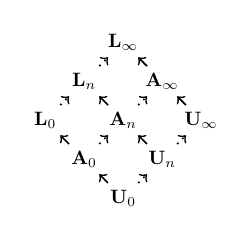
\begin{tikzpicture}
    [->,auto,semithick, every node/.style={scale=0.7}]
    \node(U) {$\kun_0$} ;
    \node(A) [above left of=U] {$\kaff_0$} ;
    \node(L) [above left of=A] {$\klin_0$} ;
    \node(Un) [above right of=U] {$\kun_n$} ;
    \node(An) [above left of=Un] {$\kaff_n$} ;
    \node(Ln) [above left of=An] {$\klin_n$} ;
    \node(Uinf) [above right of=Un] {$\kun_\infty$} ;
    \node(Ainf) [above left of=Uinf] {$\kaff_\infty$} ;
    \node(Linf) [above left of=Ainf] {$\klin_\infty$} ;
    \path
    (U) edge (A)
    (A) edge (L)
    (Un) edge (An)
    (An) edge (Ln)
    (Uinf) edge (Ainf)
    (Ainf) edge (Linf)
    ;
    \path[dotted]
    (U) edge (Un)
    (A) edge (An)
    (L) edge (Ln)
    (Un) edge (Uinf)
    (An) edge (Ainf)
    (Ln) edge (Linf)
    ;
  \end{tikzpicture}
\end{minipage}

%%% Local Variables:
%%% mode: latex
%%% TeX-master: "../main"
%%% End:

  \vspace{-5pt}
  \caption{Lattice ordering -- $k \lk_\Lat k'$}
  \label{sdtyp:lattice}
  \vspace{-10pt}
\end{figure}

\paragraph{Environments and bindings}
\label{sdtyping:envs}

\begin{figure}[tp]
  \begin{align*}
    \E &::=\ \Eempty \mid \E;B\tag{Environments}\\
    B &::=\ \bnone % \tag{Empty} \\
    \mid \bvar{\tvar}{\kschm} % \tag{Types}
    \mid \bvar{x}{\schm}% \tag{Variables}
    \mid \bvar{\borrow{x}}{\borrowty{k}{\tau}}% \tag{Borrows}\\
    \mid \svar{x}{\schm}^n % \tag{Suspended}
    % |&\ \tydecl{t}{\kschm}{K}{\tau}\tag{Type Declaration}\\
  \end{align*}
  \vspace{-10pt}
  \caption{Type environments}
  \label{grammar:env}
  \vspace{5pt}
  % \begin{minipage}{0.5\linewidth}
  \centering
    \begin{tabular}
  {@{}>{$}r<{$}@{ $\vdash_e$ }
  >{$}c<{$}@{ $=$ }
  >{$}c<{$}@{ $\ltimes$ }
  >{$}c<{$}r}

  \Cleq{\schm}{\kun_\infty}
  &\bvar{x}{\schm}&\bvar{x}{\schm}&\bvar{x}{\schm}
  &(Both)\\

  {\Cempty}&
             {\bbvar[\IBORROW]{x} k \schm}&
                                            \bbvar[\IBORROW]{x}
                                            k{\schm}&{\bbvar[\IBORROW]{x}
                                                      k {\schm}}
  &(Borrow)
  % \\
  
  % {\Cempty}&
  % \svar[\IBORROW]{x}{\schm}^n&\svar[\IBORROW]{x}{\schm}^n&\svar[\IBORROW]{x}{\schm}^n
  % &BothS
  \\[2mm]

  {\Cempty}&{B_x}&{B_x}&{\bnone}
  &(Left)\\
  {\Cempty}&{B_x}&{\bnone}&{B_x}
  &(Right)\\[2mm]

  {\Cempty}&{\bvar x \schm}&{\svar x \schm^n}&{\bvar x \schm}
  &(Susp)\\

  {\Cempty}&
             {\bbvar x k \schm}&{\svar[\IBORROW] x \schm^n}&{\bbvar x k \schm}
  &(SuspB)\\

  {\Cempty}&
             {\svar{x} \schm^{n'}}&{\svar[\IBORROW] x \schm^n}&{\svar{x} \schm^{n'}}
  &(SuspS)\\
\end{tabular}
%%% Local Variables:
%%% mode: latex
%%% TeX-master: "../main"
%%% End:

    \vspace{-5pt}
    \caption{Splitting rules for bindings -- $\lsplit{C}{B}{B_l}{B_r}$}
    \label{sdtyp:split}
  \vspace{-10pt}
  % \end{minipage}
\end{figure}


\begin{figure*}[tp]
  % \begin{minipage}{0.7\linewidth}
    \begin{mathpar}
      \ruleSDVar
      \and
      \ruleSDApp
      \and
      \ruleSDRegion
      \and
      \ruleSDBorrow
      \and
      \ruleSDLam
      \and
      \inferrule[BorrowBinding]{
        \entail{C}{(\BORROW_n\lk k) \wedge (k \lk \BORROW_\infty)}\\
        \BORROW\in\left\{\kun,\kaff\right\}
      }{
        \lregion{C}{}
        {\svar[\BORROW]{x}{\tau}^n}
        {\bvar{\borrow[\BORROW]{x}}{\borrowty[\BORROW] k{\tau}}}
      }
      % \and
      % \ruleSDPair
      % \and
      % \ruleSDMatchPair
    \end{mathpar}
    \vspace{-10pt}
    \caption{Selected typing rules ($\inferS{C}{\E}{e}{\tau}$)
      and borrowing rules ($\lregion{C}{x}{\E}{\E'}$)}
    \label{selectrules:borrow}
    \label{selectrules:binders}
    \label{sdtyp:app}
    \label{selectrules:region}
    \label{env:rule:borrow}
    \vspace{-5pt}
  % \end{minipage}
\end{figure*}

\lang controls the use of variables by supporting new modes of
binding in type environments $\E$, as defined in \cref{grammar:env}.
Environments contain standard bindings of type variables to kind schemes,
$\bvar{\tvar}{\kschm}$, value bindings $\bvar{x}{\schm}$, but also
suspended and borrow bindings.
A suspended binding, $\svar{x}{\schm}^n$, indicates that $x$ is
earmarked for a borrowing use in a nested region
marked with $x$ % (see \cref{sdtyping:regions}),
but
cannot be used directly.
A borrow binding, $\bvar{\borrow{x}}{\borrowty{k}{\schm}}$, replaces
such a suspended binding on entry to the $x$-region. It indicates
that the borrow $\borrow{x}$ can be used directly. Kind $k$
restricts the lifetime of the borrow to the region (see \cref{selectrules:borrow}).

% , either
% through
% linearity and affinity which restrict how variables are shared and ignored,
% or through borrows which allow to circumvent the linearity rules
% in a controlled way.
% In order to check these properties, we introduce several new bindings
% in our typing environments.
% The grammar of type environment (denoted $\E$) is shown in \cref{grammar:env}.

% Environments are also used to encode several linearity-related properties
% through \emph{environment-wide constraints}.
Constraints on an environment control substructural properties by
restricting the types of variables.  The constraint $\Cleq{\E}{k}$
abbreviates $\Cleq\schm k$, for all $\bvar{x}{\schm}$
% $\svar{x}\schm$, and $\bvar{\borrow{x}}{\borrowty{k'}{\schm}}$
in $\E$, which in turn means that $k' \lk k$ where $k'$ is the kind of
the variable's type scheme.
Borrow bindings follow the exact same rules, but suspended bindings
are forbidden in an environment $\E$ constrained like that.
This intuitive explanation is sufficient to understand
the {\sc Abs} and {\sc Var} rules shown in
\cref{selectrules:binders}.

The {\sc Var} rule looks up the type scheme of the variable $x$ in
the environment $\E$
and instantiates it using the substitution $\unif$. The rule also
checks that the other bindings in $\E$ can be safely discarded by
imposing the constraint $\Cleq{\E\Sdel{x}}{\kaff_\infty}$.
It enforces that all remaining bindings (except $x$) are affine or
unrestricted and can therefore be discarded.

The {\sc Abs} rule ensures that the kind annotation on the arrow type
($\tau_2 \tarr{k} \tau_1$) reflects the restrictions on the captured variables.
To do so, the rule imposes the constraint $\Cleq\E k$.
If, for instance, any binding in $\E$ is affine, it gives rise to the
constraint $\Cleq{\kaff_n}{k}$, so that  the arrow kind is at least
affine at nesting level $n$.
Capturing a borrow is perfectly fine: the kind of the borrow is also a
lower bound of the arrow kind $k$ which restricts the closure
to the region of the borrow.
Capturing a suspended binding is forbidden.
% Note that $x$ is \emph{not} included in $\E$: since it's the argument of the
% closure, its use should not induce a capture.




\paragraph{Copying and Splitting}
\label{sdtyping:split}

The {\sc App} typing rule in \cref{sdtyp:app} demonstrates how \lang
deals with duplication and dropping of values.
The splitting $\lsplit{C}{\E}{\E_1}{\E_2}$ in the rule decomposes the
type environment $\E$ in two parts, $\E_1$ and $\E_2$, which are used
to typecheck the components of the pair.
% The constraint $C$ characterizes a valid  splitting.

\cref{sdtyp:split} shows the action of splitting rules on single
bindings. If $x$'s type is unrestricted,
rule {\sc Both} indicates that we can duplicate it.
Similarly, unrestricted borrows can be duplicated with rule
{\sc Borrow}.
{\sc Left} and {\sc Right} rules are always applicable and move a binding
either to the left or right environment.
The rules {\sc Susp}, {\sc SuspB} and {\sc SuspS}
split off suspended bindings to
the left while conserving access to the binding on the right.
A suspended binding can later be turned
into a borrow inside a region. Splitting of suspended bindings is
asymmetric. It must follow the order of execution from left to right,
which means that a resource can be used first as a borrow on the left
and then later as a full resource on the right. The {\sc Susp} rule
works with a full resource, the {\sc SuspB}
with a borrow and {\sc SuspS} with a suspended binding.

Splitting applies whenever an
expression has multiple subexpressions:  function applications,
and let bindings. In the
expression
$\letin{a}{\text{create}\ 8\ x}
{f\ \region[{}]{\Sone a\IBORROW}{\text{length}\ \borrow[\IBORROW]{a}}\ a}$,
the rule {\sc Susp} splits off a borrow from  the resource
$a$ to use it in the left argument.
As usual, a borrow cannot be active in the same scope as its resource.
The \emph{region} around its use ensures that the borrow in the left argument
does not
escape, which brings us to the next topic.


% \paragraph{Pattern matching}
% \label{sdtyping:matching}

% Elimination of pairs is done using a matching construct
% $(\matchin{x,x'}{e_1}{e_2})$ whose
% typing rule is shown in \cref{selectrules:matching}.
% This construction can eliminate both normal pairs, but also borrows
% of pairs.
% A syntactic marker $\etransfm$ indicates if it applies to
% a pair ($\etransfm = \operatorname{id}$) or a borrow ($\etransfm = \&^\BORROW$).
% If $\etransfm = \operatorname{id}$, the typing simplifies to
% a regular destruct on pairs.
% Otherwise, $e_1$ is expected to be of type
% $\borrowty{k}{\tyPair{\tau_1}{\tau'_1}}$
% while $x$ and $x'$ are of type respectively
% $\borrowty{k}{\tau_1}$ and $\borrowty{k}{\tau'_1}$.

% Matching is voluntarily simple here and
% could be improved using a richer pattern language
% to access inner components and a typeclass mechanisms
% to avoid the need for explicit markers for borrow matches.
% Both extensions are compatible with our system and have been partially
% implemented in our prototype type-checker.

\paragraph{Regions}
\label{sdtyping:regions}

% \begin{figure}[tp]
%   % \begin{minipage}{0.4\linewidth}
%   %   \centering
%   %   \begin{mathpar}
%   %     \ruleSDRegion
%   %   \end{mathpar}
%   %   \caption{The {\sc Region} rule}
%   %   \label{selectrules:region}
%   % \end{minipage}\hfill
%   % \begin{minipage}{\linewidth}
%     \centering
%     % \begin{tabular}
%     %   {@{}>{$}r<{$}@{ $\vdash_e$ }
%     %   >{$}c<{$}@{ $\rightsquigarrow_n^{x}$ }
%     %   >{$}l<{$}
%     %   r}

%     %   (\kun_n\lk k\lk\kun_\infty)
%     %   &{\svar[\IBORROW]{x}{\tau}^n}
%     %   &{\bvar{\borrow[\IBORROW]{x}}{\borrowty[\IBORROW] k{\tau}}}
%     %   &Immut\\

%     %   (\kaff_n\lk k\lk\kaff_\infty)
%     %   &\svar[\MBORROW]{x}{\tau}^n
%     %   &\bvar{\borrow[\MBORROW]{x}}{\borrowty[\MBORROW] k{\tau}}
%     %   &Mut
%     % \end{tabular}
%     \begin{mathpar}
%     \end{mathpar}
%     \vspace{-10pt}
%     \caption{Borrowing rules for bindings -- }
%   \vspace{-10pt}
%   % \end{minipage}
% \end{figure}

Borrowing is crucial to support an imperative programming style.
To guarantee the validity of a borrow, its lifetime must be properly contained in its
ancestor's lifetime. \lang ensures proper nesting of lifetimes by using
regions. The expression $\region{\Sone x\BORROW}{e}$ indicates a
region at nesting level $n$ in which a $\BORROW$-borrow can be taken of $x$.

The typing for a region (see the {\sc Region} rule in \cref{selectrules:region})
replaces suspended bindings by borrow bindings
(\cref{env:rule:borrow}), typechecks the body
of the region, and finally ensures that the borrow does not leak outside.
This last check is done with indices that correspond to the nesting
level of the region. The kind $k$ of the borrow is indexed with the level $n$
corresponding to its region, thanks to the constraint $(\BORROW_n\lk
k)$, and the constraint $\Cleq{\tau}{\klin_{n-1}}$ ensures that
the return type of the region must live at some enclosing, lower level.

As an example, consider the expression $\region{\Sone x\IBORROW}{f(\borrow[\IBORROW]{c})}$
where $c$ is a linear channel in an environment $\E$.
The first step is to check that $\svar[\IBORROW]{c}{\text{channel}}$
is in $\E$.
When entering the region, rule \TirName{Region} imposes
$\lregion{C}{x}{\E}{\E'}$, which defines $\E'$
corresponding to $\E$ where the suspended binding is replaced by the
borrow binding  $\bvar{\borrow[\IBORROW]{c}}{\borrowty[\IBORROW]{k}{\text{channel}}}$.
To constrain the borrow to this region we impose the constraint
$\entail{C}{(\kun_n\lk k) \wedge (k \lk\kun_\infty)}$, which affirms
that the borrow is unrestricted, but can only be used in nesting
levels $n$ and higher.
%
% With that setup we typecheck the body of the region,
% $f(\borrow[\IBORROW]{c})$.
% The constraint $\Cleq{\tau}{\klin_{n-1}}$ ensures
% that the kind of $\tau$ does not contain anything whose kind is
% ``above level $n$'' and thus confines the borrow to the region
% (for instance, $\borrowty[\IBORROW]{\kun_n}{\text{c}}$ has kind
% $\kun_n$ and thus cannot be returned).
%
The \TirName{Region} rule also imposes the constraint
$\Cleq{\tau}{\klin_{n-1}}$, which prevents the borrow, having kind $k$ of level
$\geq n$, from escaping the region's body of type $\tau$.


% As it would be cumbersome to markup regions manually, we developed an
% algorithm that starts from each borrow, creates a region around it,
% and extends it as much as possible while respecting other borrows
% and binders. The algorithm (see \cref{regionannot}) also provides the region's level
% and variable annotation.
% Henceforth, we consider terms with fully annotated regions.



% \paragraph{Kind checking}

% \TODO{Present this if we have enough space}

\paragraph{Resource management}

As a model of resource, we consider a simple abstract
type $\tapp{\tres}{\tau}$ whose content of type $\tau$ must be $\kun_0$ and
equipped with four operations:
\begin{itemize}
\item
$\create$:
$\forall{\kvar_\tvar}\bvar{\tvar}{\kvar_\tvar}.\
\qual{\Cleq {\kvar_\tvar} {\kun_0}}
{\tvar \tarr{} \tapp\tres\tvar}$\\
Creates a new resource.

\item
$\observe$:
$\forall{\kvar\kvar_\tvar}\bvar{\tvar}{\kvar_\tvar}.\
\qual{\Cleq {\kvar_\tvar} {\kun_0}}
{\borrowty[\IBORROW]{\kvar}{\tapp\tres\tvar} \tarr{} \tvar}$\\
Reads from a shared borrow of a resource.

\item
$\update$:
$\forall{\kvar\kvar_\tvar}\bvar{\tvar}{\kvar_\tvar}.\
\qual{\Cleq {\kvar_\tvar} {\kun_0}}
\borrowty[\MBORROW]{\kvar}{\tapp\tres\tvar} \tarr{} \tvar \tarr{\kaff} \tunit$\\
Writes to an exclusive borrow of a resource.

\item
$\destroy$:
$\forall{\kvar\kvar_\tvar}\bvar{\tvar}{\kvar_\tvar}.\
\qual{\Cleq {\kvar_\tvar} {\kun_0}}
\tapp\tres\tvar \tarr{} \tunit$\\
Destroys a resource.
\end{itemize}

% \clearpage
\subsection{Semantics}
\label{sec:sem}
\begin{figure}[!tbp]
%   \begin{align*}
% \end{align*}
% \begin{minipage}[t]{0.49\linewidth}
  \begin{align*}
    \htag{Elaborated expressions}
    v ::=~& x \mid \ivar x {\Multi k} {\Multi\tau} \mid \lam[k]{x}{e} \mid \introPair[k]{v}{v'}\\
    e ::=~& x \mid \ivar x {\Multi k} {\Multi\tau} \mid \lam[k]{x}{e} \mid \introPair[k]{e}{e'}\\
    \mid~& \matchin{x,y}{e}{e'} \tag{Tagged pairs}\\
    \mid~& \letin{x}{e}{e'}\\
    \mid~& \letin{\bvar x \schm}{v}{e'}\\
    \mid~& \iapp{\Sp}{e}{e'} \tag{El. application}\\
    \mid~& \region{\Sone x\BORROW}{e}\tag{Region}\\
    \mid~& \borrow{x} \mid \reborrow{x}\tag{Borrows}\\
    \mid~& \create \mid \observe \mid \update \mid \destroy \tag{Resources}\\
    % e &::= \dots \\
    % &\mid \ilam{\Multi\kvar}{\Multi{\tvar : k}}Ckx{\tau}e \tag{El. poly abstraction} \\
    % &\mid \imlam kx{\tau}e \tag{El. mono abstraction} \\
    % &\mid \ivar x {\Multi k} {\Multi\tau} \tag{Instantiation} \\
    % &\mid \introPair[k]{e}{e} \tag{Tagged pairs}\\
    % &\mid \iapp{\Sp}{e}{e} \tag{El. application}\\
    \htag{Elaborated A-normal expressions}
    % TODO: what about constructors applied to values?
    X ::=~& x \mid \ivar x {\Multi k} {\Multi\tau}\\
    v ::=~& c \mid X \mid \lam[k]{x}{e} \mid \introPair[k]{X}{X'}\\
    E ::=~& c \mid X \mid \lam[k]{x}{e} \mid \introPair[k]{x}{x'}\\
    \mid~& \borrow{x} \mid \reborrow{x}\tag{Borrows}\\
    \mid~& \create \mid \observe \mid \update \mid \destroy \tag{Resources}\\
    \mid~& \app{x}{x'} \tag{El. application}\\
    e ::=~& \letin{x}{E}{e'}\\
    \mid~& \letin{\bvar x \schm}{v}{e'}\\
    \mid~& \matchin{x,y}{z}{e} \tag{Tagged pairs}\\
    \mid~& \region{\Sone x\BORROW}{e}\tag{Region}\\
    \htag{Environment}
    \Addr ::=~& \Multi\IBORROW\Multi\MBORROW\Loc \tag{Locations}
    % \\           &\mid \borrow{\Addr} \tag{Borrows}
    \\
    \Perm ::=~& \{\} \mid \Perm + \Addr \tag{Permissions}
    \\
    r ::=~& \Addr \mid c \tag{Results}\\
    \VEnv ::=~& \Eempty \mid \VEnv( x \mapsto r) \tag{Enviroments} \\
%   \end{align*}
% \end{minipage}
% \hfill
% \begin{minipage}[t]{0.49\linewidth}
%   \begin{align*}
    \htag{Storables}
    w ::=~& \StPClosure \VEnv {\Multi\kvar} C k x e \tag{Poly Closures}\\
    \mid~& \StClosure \VEnv k x e \tag{Closures} \\
    \mid~& \StPair k r r \tag{Pairs} \\
    \mid~& \StRes r \tag{Resources} \\
    \mid~& \StFreed \tag{Freed Resource}
    \\
    \htag{Store}
    \Store ::=~& \Eempty \mid \Store( \Loc \mapsto w)
    \\
    \htag{Splittings}
    \Sp ::=~& \Multi{\SpBoth \mid \SpBorrow \mid \SpLeft \mid \SpRight \mid \SpSusp \mid \SpSuspB}
  \end{align*}
% \end{minipage}
\caption{Syntax of internal language}
\label{fig:syntax-internal-language}
\end{figure}

%%% Local Variables:
%%% mode: latex
%%% TeX-master: "main"
%%% End:


\lstMakeShortInline[keepspaces,style=rule,basicstyle=\normalsize\normalfont]@

The dynamics of \lang is given in big-step
functional
style~\cite{siek13:_type_safet_three_easy_lemmas,DBLP:conf/esop/OwensMKT16,
  DBLP:conf/popl/AminR17}.  A function
@eval \Store \Perm \VEnv i e@
manipulates the semantic objects defined in
\cref{fig:syntax-internal-language}.
% To demonstrate resource handling, the semantics comes with an abstract
% notion of linear resources that can be created, destroyed, observed
% (through unrestricted borrows), and
% updated (through affine borrows).
%
The semantics is defined in terms of \emph{elaborated expressions} $e$
with kind, constraint, and splitting annotations inserted by the typechecker.
A splitting $\Sp$ is evidence of the splitting relation for type environments
used in the typing rules.

Let-polymorphism is demonstrated for functions giving rise to elaborated
$\eletfun$ expressions annotated with a type scheme $\schm$ and a kind $k$ indicating their
usage restriction (linear, affine, etc) relative to the variables and
constraints of $\schm$. Their use
gives rise to explicit instantiation of the kind and type variables.
% Pairs come with a kind tag $k$ indicating the usage restriction.

Addresses $\Addr$ are composed of a raw location $\Loc$, which is just
a pointer into a store, and a stack of modifiers that indicates the
borrows that have been taken from the original object. From the raw
location, we may take affine borrows and reborrows. Once we have
taken an unrestricted borrow (from a raw location or a borrowed one),
then we can take further unrestricted borrows from it, but no more
affine ones.

A permission $\Perm$ is a set of addresses that may be accessed during
evaluation. A well-formed permission contains at most one address for each raw
location.

Non-trivial results are boxed in the  semantics. So, a result
$r$ is either an address or a primitive constant (e.g., a number).

A value environment $\VEnv$  maps variables to results.

A storable $w$ describes the content of a location in the store. There are five
kinds of storables. A \emph{poly closure} represents a polymorphic
function. It consists of an environment and the components of an
elaborated abstraction. A \emph{closure} represents a monomorphic
function in the usual way. A \emph{pair}
consists of a kind and two results. A \emph{resource} contains
a result and the \emph{hole} $\StFreed$ fills a released location.

A store $\Store$ is a partial map from raw locations to
storables. The function
@salloc: store -> storable -> (loc * store)@ is such that
@salloc delta@ @w@ allocates an unused location in @delta@ and fills it with
@w@. It returns the location and the extended store.


The evaluation function is indexed by a step count @i@ so that each
invocation is guaranteed to terminate either with an error, a timeout,
or a result. Its return type is a monad
@'a sem@ which combines error reporting and timeout:
\begin{lstlisting}
type 'a sem = Error of string | TimeOut | Ok of 'a
val eval: store->perm->venv->int->exp->(store*perm*result) sem
\end{lstlisting}
It evaluates the given expression in the context of an initial store, a
permission to use addresses in the store, a value environment, and a
step count. If successful, it returns the final store, the remaining
permissions, and the actual result.

\begin{figure}
  \lstsemrule{varinst}
  \medskip
  \lstsemrule{sapp}
  \medskip
  \lstsemrule{spair}
  \medskip
  \lstsemrule{sregion}
  \caption{Big-step Interpretation}
\end{figure}


%%% Local Variables:
%%% mode: latex
%%% TeX-master: "main"
%%% End:


We give some excerpts of the definition of @eval@ in
\cref{fig:big-step-interpretation} and leave the full
definition for \cref{sec:semant-defin}.
% The appendix also
% contains the semantics in mathematical notation.
The definition uses OCaml syntax with some pretty
printing. The pervasive @let*@ operator acts as monadic bind
for the @sem@ monad. The operator
@let*? : bool -> (unit -> 'a sem) -> 'a sem@
 converts a boolean
argument into success or failure in the monad.
 The function header of @eval@ checks
whether time is up and otherwise proceeds processing the expression.

The @Varinst@ case corresponds to instantiation. It
obtains the variable's value, checks that it is a location, checks the
permission (the @let*?@ clause), obtains the storable $w$ at that
location, and checks that it is a poly closure (STPOLY). Next, it updates the
permission: if the poly closure is unrestricted, then the location
remains in the permission set, otherwise it is removed. Finally, we
allocate a new monomorphic closure, add it to the permissions, and
return the pointer as the result along with the updated store and
permissions.

The @App@ case implements (elaborated) function application.
We first apply the splitting @sp@ to @gamma@ and
evaluate subterm @e_1@ with its part of the environment and the
decremented timer @i'@. The result must be a location that we are
permitted to use. Moreover, there must be a monomorphic STCLOS stored
at that location. The permission to further use this closure  remains
in force only if the closure is unrestricted. Finally, we evaluate the
argument, then the function body, and return its result.

% The @Pair@ case corresponds to the \TirName{Pair} typing rule. It
% requires no new features.


The @Region@ case implements a region. It obtains the address for @x@,
the suspended binding, and extends it with the intended borrow
$\BORROW$. This extension may fail if we try to take an affine borrow
of an unrestricted borrow. Next, we rebind @x@ to the borrow's
address, extend the permission accordingly, and execute the region's
body.  Finally, we withdraw the permission and return the result.

The @Borrow@ case obtains the address for @x@, checks that it is a
borrow of the correct mode $\BORROW$ and whether it is permitted to
use it. It just returns the address.

\lstDeleteShortInline@

%%% Local Variables:
%%% mode: latex
%%% TeX-master: "main"
%%% End:

\section{Inference}
\label{inference}

An important contribution of \affe is its principal type inference.
We now formulate our inference algorithm
based on the $HM(X)$ framework~\citep{DBLP:journals/tapos/OderskySW99}.
$HM(X)$ is a Hindley-Milner type system for a language
with qualified types where constraints are expressed in an arbitrary
theory $X$.
Most important, given some properties on the constraint system $X$,
$HM(X)$ ensures principal type inference.
We apply HM(X) to a concrete constraint language which we name $\CL$.
We adapt and extend its existing rules to support kind inference,
track linearity and handle borrows and regions. Finally, we
formulate an appropriate constraint solving algorithm for $\CL$.
In addition, our constraint solving algorithm simplifies constraints in a
principled way.
We first present various preliminary definitions
before showing our kind and type inference judgements
and our constraint solving algorithm.

\subsection{Preliminaries}

Unlike the syntax-directed version of our type system, knowing which elements
are input and output or our inference judgement is critical. In the rest
of this section, when presenting a new judgement
we will note in \textbf{bold} the input parameters. The rest will then be
output parameters.

\subsubsection{Usage environments}

% One novelty of our inference  judgement now
% returns a type environment, which we call ``usage environment'' and commonly
% note $\Sv$, to summarize how variables and borrows are used inside
% the expression.

In order to determine if a variable is used in an affine manner, we must track
its uses and the associated kinds. For instance, in the expression
$(x,x)$, $x$ is used twice. If $x$ is of type $\tau$, which is of kind $k$,
we must add the constraint $\Cleq{k}{\kun}$.
%
In order to infer such constraints, our inference judgement will not only
take an environment as parameter but also return an environment, which
we call ``usage environment'', and which summarize how variables and borrows
are used. Usage environments follow the exact same grammar
as normal environment. In order to distinguish them more easily,
we note them $\Sv$.

In \cref{sdtyping}, we used various relations to split environments in two, or
transform suspended bindings into borrow binding inside an environment.
These relations took as argument a constraint which is used to validate
the environment transformation.
In the context of inference, we define a new judgements which \emph{infers}
the constraints required.
\begin{itemize}
\item $\bsplit{C}{\Sv}{\bf{\Sv_1}}{\bf{\Sv_2}}$.
  Given two usage environments (inferred for two subexpressions, for instance)
  $\Sv_1$ and $\Sv_2$, we return $\Sv$, the merged environment, and $C$, a set
  of constraints that must be respected.
  This relation is total and non-ambiguous given $\Sv_1$ and $\Sv_2$
  and uses the same rules as the one presented in \cref{sdtyping:split}.
\item $\bregion{C}{\bf{x}}{\Sv}{\bf\Sv'}$.
  Given a usage environment $\Sv'$ and a variable name $x$, we return
  $\Sv$ where the borrow binding of $x$ in $\Sv'$, if it exists, is replaced by
  a suspended binding. We also return $C$, a set of constraints that must
  be respected.
  Again, the relation is total and non-ambiguous for any given $\Sv'$ and $x$,
  and uses the same rules as the one presented in \cref{sdtyping:regions}.
\end{itemize}

The relations used for syntax-directed typing can trivially be defined
in term of these new relations and constraint entailment.
All relations are fully described in \cref{typ:extra:envs}.

\subsubsection{Constraint normalization}

The HM(X) framework assumes the existence of a $\operatorname{normalize}$
function which takes a constraint $C$ and a substitution $\psi$ and returns a
simplified constraint $C'$,
and an updated substitution $\unif'$.
Normalization is supposed to return the ``best'' solution $(C',\unif')$, for
instance the most general unifier.
We detail the implementation
of the normalization function and its property in \cref{infer:solving}.
In the meantime, we simply
assume the existence of such a function for our constraint system.

\subsection{Kind inference}

We note $\inferK{(C,\unif)}{\bf{\E}}{\bf{\tau}}{k}$ when type $\tau$ has kind $k$
in environment $\E$ under constraints $C$ and unifier $\unif$.
$\E$ and $\tau$ are the input parameters of
our inference procedure.
We present the kind inference algorithm as a set of rules in
\cref{rules:kinding}.
Similar to the syntax-directed rules, higher-kinds are not generally supported
and can only appear by looking-up the kind scheme of a type constructor,
for use in the type application rule {\sc KApp}.
Type variables must be of a simple kind in rule {\sc KVar}.
Kind schemes are instantiated in the {\sc KVar} rules by creating
fresh kind variables and the associated substitution.
{\sc KArr} and {\sc KBorrow} simply returns the kind of the primitive
arrow and borrow types.
The $\operatorname{normalize}$ function is used every time several constraints
must be composed in order to simplify the constraint and return a most general
unifier.

\begin{figure}[ht]
  \centering
  \begin{mathpar}
  \inferrule[KVar|KCons]
  { \bvar{\tvar|\T t}{
      \forall \kvar_i.\ \qual{D}{(\Multi[j]{k}) \karr k}}
    \in \E \\
    \Multi[i]{\kvar'} \text{ fresh} \\\\
    (C,\unif) =
    \normalize{D}{\subst{\kvar_i}{\kvar'_i}{}_i}
  }
  { \inferK{(C,\unif|_{\fv{\E}})}{\E}{\tvar|\T t}{\unif ((\Multi[j]{k}) \karr k)} }
  \and
  \inferrule[KArr]
  { }
  { \inferK{(\Ctrue,\emptyset)}{\E}{\tau_1 \tarr{k} \tau_2}{k} }
  \and
  \inferrule[KBorrow]
  { }{ \inferK{(\Ctrue,\emptyset)}{\E}{\borrowty{k}{\tau}}{k}}
  \and
  \inferrule[KApp]
  { \forall j,\
    \inferK{(C_j,\unif_j)}{\E}{\tau_j}{k'_j} \\
    \inferK{(C_0,\unif_0)}{\E}{\T t}{(\Multi[j]{k}) \karr k}
    \\\\
    (C,\unif) =
    \normalize
    {C_0\Cand \Multi[j]{C} \Cand \Multi[j]{\Ceq{k'_j}{k_j}}}
    {\unif_0\meet \Multi[j]{\unif}}
  }
  { \inferK{(C,\unif|_{\fv{\E}})}{\E}{\tapp{\tcon}{\Multi[j]{\tau}}}{\unif k} }
  \and
  \inferrule[KPair]
  { \forall i,\
    \inferK{(C_i,\unif_i)}{\E}{\tau_i}{k_i} \\
    \kvar \text{ fresh} \\\\
    (C,\unif) =
    \normalize
    {\Multi[i]{C} \Cand \Multi[i]{\Cleq{k_i}{\kvar}}}
    {\Multi[i]{\unif}}
  }
  { \inferK{(C,\unif)}{\E}{\tyPair{\tau_1}{\tau_2}}{\unif\kvar} }
\end{mathpar}


%%% Local Variables:
%%% mode: latex
%%% TeX-master: "../main"
%%% End:

  \caption{Kind inference algorithm -- $\inferK{(C,\unif)}{\E}{\tau}{k}$}
  \label{rules:kinding}
\end{figure}



\subsection{Type inference}

We note $\inferW{\Sv}{(C,\unif)}{\bf{\E}}{\bf{e}}{\tau}$ when
$e$\ has type $\tau$ in $\E$ under the constraints $C$ and unifier $\unif$
with a usage environment $\Sv$. $\E$ and $e$ are the input parameters of our
inference algorithm.
We revisit the syntax-directed rules presented in \cref{sdtyping} to highlight the
novelties
of our inference algorithm and the differences with the syntax-directed
system.
As before, the complete type inference rules are shown in \cref{appendix:infer}.

\subsubsection{Environments and bindings}
\label{infer:envs}

In our syntax directed system presented in \cref{sdtyping}, we ensured
that linear variables are not discarded at the \emph{leafs}, through
the {\sc Var} rule. In the inference algorithm, we operate in the opposite
direction: we collect data from the leafs, and only enforce linearity
at \emph{binders}. This is reflected in the {\sc Var$_I$} and
{\sc Abs$_I$} rules presented in \cref{rule:infer:envs}.
Typing for variables is very similar to traditional (non-affine) ML
typing. The only difference is that we collect
the fact that $x$ was used with the scheme $\schm$ by returning
a usage environment $\Sv = \{ \bvar{x}{\schm} \}$.
%
This usage environment is in turn used at each binder to enforce proper
usage of linear variable via the $\Weaken$ property.
We demonstrate how this is achieved for lambda expressions
in the {\sc Abs$_I$} rule.
First, we typecheck the body of the lambda and obtain a usage
environment $\Sv_x$. Just like in the syntax directed,
we introduce the constraint
$\Cleq{\Sv\Sdel{x}}{\kvar}$ which properly accounts for captures in
the body of the lambda expression. We also introduce the constraint
$\Weaken_{\bvar{x}{\sigma}}(\Sv)$. If $x$ was used $e$, $x$ is present
in $\Sv$ and this constraint is empty. Otherwise, if $x$ is
\emph{not} present in $\Sv$, its type should not have a linear
kind, which is enforced by the constraints $\Cleq{\sigma}{\kaff_\infty}$.
The $\Weaken$ constraint is introduce at each binding point in the program
such as let-bindings and pattern matching.

Note again here the use of normalization on complex constraints to ensure
that the inference algorithm always return the simplest possible
constraints and unifiers.

\begin{figure}[!h]
  \begin{mathpar}
    { \Weaken_{\bvar{x}{\sigma}}(\Sv) =
      \begin{dcases}
        \Ctrue&\text{if } x\in\Sv\\
        \Cleq{\sigma}{\kaff_\infty}&\\
      \end{dcases}
    }
    \and
    \ruleIVar
    \and
    \ruleIAbs
  \end{mathpar}
  \caption{The {\sc Abs$_I$} and {\sc Var$_I$} rules}
  \label{rule:infer:envs}
\end{figure}


\subsubsection{Splitting and Regions}
\label{infer:split}
\label{infer:regions}


As noted previously, in our inference algorithm, we infer
usage environments which describes how variables are used. In
\cref{sdtyping}, we described the {\sc Pair} and {\sc Region} rules, and their
respective actions on the environment. We now see the inference version
of these rules in \cref{rule:infer:envrules}.
While the rules are quite similar to the original version, the usage
environment $\Sv$ is now an \emph{output} of the algorithm.
As such, we use the ``inference'' version of the relations on
environment,
$\bsplit{C}{\Sv}{\bf{\Sv_1}}{\bf{\Sv_2}}$ and $\bregion{C}{\bf{x}}{\Sv}{\bf\Sv'}$,
which returns the necessary constraints and
are total and non ambiguous for their input parameters ($\Sv_1, \Sv_2$ and $\Sv'$, respectively).
We then simply collect all the constraints and normalize them.

\begin{figure}[!h]
  \centering
  \begin{mathpar}
    \ruleIPair
    
    \ruleIRegion
  \end{mathpar}
  \caption{The {\sc Pair$_I$} and {\sc Region$_I$} rules}
  \label{rule:infer:envrules}
\end{figure}

\subsubsection{Generalization and constraints}


So far, constraints have only been composed of a list of kind inequalities.
The internal language of constraints used for inference is in fact
richer.
To illustrate this, we now show the inference rule for let-bindings
in \cref{rule:infer:let}.
This rule combines several ingredients previously seen:
since let expressions are binders, we use $\Weaken$ on the bound
identifier $x$. Since let-expressions contain
two subexpressions, so we use the environment splitting relation,
$\bsplit{C_s}{\Sv}{\Sv_1}{(\Sv_2 \Sdel{x})}$. We carefully remove the $x$ from
the left environment, since it is not available outside of the expression
$e_2$, and thus should not be part of the returned usage environment.

As per tradition in ML languages, generalization is performed
on let-bindings.
Following HM(X), we note $(C_\schm, \schm) = \generalize{C}{\E}{\tau}$
the pair of a constraint and a scheme resulting from
generalization. The definition is provided in \cref{rule:infer:let}.
The type scheme $\schm$ is created by quantifying over all the appropriate
free variables and the current constraints.
The generated constraint $C_\schm$ uses a new projection operator,
noted $\Cproj{\tvar}{D}$, which
allow the creation of local variables inside the constraints.
This allow to encapsulate all the quantified variables in the global constraints.
It also reflect the fact that there
should exists at least one solution for $C$ for the scheme to be valid.
\citet{DBLP:journals/tapos/OderskySW99} give a detailed account
on the projection operators in HM inference.

\begin{figure}[!h]
  \centering
  \begin{mathpar}
    \ruleILet

    {\generalize{C}{\E}{\tau} =
      (\Cproj{\Multi{\kvar},\Multi{\tvar}}{C},
      \forall \Multi{\kvar},\Multi{\tvar}.\qual{C}{\tau})

      \text{ where }

      \Multi{\kvar},\Multi{\tvar} = (\fv{\tau}\cup\fv{C})\setminus\fv{\E}
    }
  \end{mathpar}
  \caption{The {\sc Let$_I$} rule}
  \label{rule:infer:let}
\end{figure}

\subsection{Constraint solving}
\label{infer:solving}

\newcommand\A{\mathcal A}
\newcommand\SC{\mathcal S}

Before presenting our constraint solving algorithm,
we place ourselves in a more general context where kinds are either variables
or constants belonging to a total bounded lattice $(\mathcal L, \lk_\Lat)$ ie.,
a lattice which admits a total order and upper and lower bounds ($l^\top$ and $l^\bot$).
We note lattice elements $l$ and $\glb_i l_i$ (resp. $\lub_i l_i$)
the greatest lower bound (resp. least upper bound) in $\mathcal L$.
The lattice used in \lang which was presented
in \cref{sdtyping} is a total bounded lattice with
$l^\top = \klin_\infty$ and $l^\bot = \kun_0$.
%
Let $\CL$ the set of constraints in such arbitrary lattice $mathcal L$.
The full grammar of constraints is shown in \cref{grammar:constraint}.
Constraints are made of kind inequalities, conjunctions and
projections, as shown previously, along with type unification
constraints. Since types might contain kinds (for instance, on the arrows),
type unification is oriented and noted $\leq$.
For simplicity, we consider all type constructors
invariant in their parameters
and define $\Ceq{\tau}{\tau'}$ as $\Cleq{\tau}{\tau'} \wedge \Cleq{\tau'}{\tau}$.

As before, entailment is noted $\entail{C}{D}$,
where $D$ is a consequence of the constraints $C$.
We say that $C$ and $D$ are equivalent, noted $C \equivC D$,
when $\entail{C}{D}$ and $\entail{D}{C}$.
The base rules for entailment are given in \cref{rules:entail}.
The rules for classic Herbrand unification and
projection operators are omitted for brevity (see
\citep{DBLP:journals/tapos/OderskySW99} for
details).

\begin{figure}[!bt]
  \centering
  \begin{minipage}{0.32\linewidth}
    \begin{align*}
      C &::= \Cleq{\tau_1}{\tau_2} \\
        &\mid \Cleq{k_1}{k_2} \tag{Inequalities} \\
        &\mid C_1 \Cand C_2  \tag{Conjunction}\\
        &\mid \Cproj{\tvar}{C} 
        \mid \Cproj{\kvar}{C} \tag{Projection} 
    \end{align*}
    \caption{The constraint language}
    \label{grammar:constraint}
  \end{minipage}\hfill
  \begin{minipage}{0.66\linewidth}
    \begin{mathpar}
      \inferrule
      {\forall i,\ \entail{C}{\Cleq{l_i}{k}}}
      {\entail{C}{\Cleq{\wedge_i l_i}{k}}}
      \and
      \inferrule
      {\forall i,\ \entail{C}{\Cleq{k}{l_i}}}
      {\entail{C}{\Cleq{k}{\vee_i l_i}}}
      \and
      \inferrule
      { \forall i,\ \entail{C}{\Ceq{\tau_i}{\tau_i}}\\
      }
      { \entail{C}{\Cleq{\tapp{t}{(\tau_i)}}{\tapp{t}{(\tau'_i)}}} }
      \and
      \inferrule{l \lk_\Lat l'}{\entail{}{\Cleq{l}{l'}}}
      \and
      \inferrule
      { \entail{C}{\Cleq{\tau'_1}{\tau_1}}\\
        \entail{C}{\Cleq{\tau_2}{\tau'_2}}\\
        \entail{C}{\Cleq{k}{k'}}
      }
      { \entail{C}{\Cleq{\tau_1\tarr{k}\tau_2}{\tau'_1\tarr{k'}\tau'_2}} }
    \end{mathpar}
    \caption{Base entailment rules -- $\entail{C}{D}$ }
    \label{rules:entail}
  \end{minipage}
\end{figure}

We define the set of solved formed
$\mathcal S$ as the set of constraints $\CL$ quantified by $\equivC$.
We will show later that such constraints are in fact only composed of
kind inequalities, and thus correspond to the syntactic constraints
used in type and kind schemes.
%
We now define our normalization procedure, noted $\normalize{C_0}{\unif_0}$ where
$C_0\in \CL$ is a set of constraints and $\unif_0$ is a substitution.
It returns a constraint $C \in \mathcal S$ in
solved form and a unifier $\unif$.
The main idea of the algorithm is to first remove all the type equalities
by using regular Herbrand unification. After that, we only have
a set of inequalities among kinds, which we can consider as a relation.
We can then saturate the relation,
unify all kinds that are in the same equivalence classes to obtain
a most general unifier on kind variables,
remove all existentially quantified variables and
then minimize back the relation and apply various
simplification rules to make the resulting type easier to understand to users.

More precisely, we apply the following steps:
\begin{enumerate}
\item Solve all type equality constraints through Herband unification and
  gather all existential quantifications at the front of the constraint.
  We obtain a constraint $C^k = \exists \kvar_i,\ \Cleq{k_j}{k'_j}_j$ and
  a substitution $\unif_\tau$.
  
  We note $\mathcal R$ the relation $\Cleq{k_j}{k'_j}_j$,
  $\mathcal G$ the underlying directed graph and $V$ its vertices.

\item Saturate the lattice equalities in $\mathcal R$.
  
  More precisely, for each kind variable $\kvar \in V$,
  for each constant $l_i$ (resp. $l_j$) such that
  there is a path from $l_i$ to $\kvar$ (resp. from $\kvar$ to $l_j$) in $\mathcal G$,
  add an edge from $\lub l_i$ to $\kvar$
  (resp. from $\kvar$ to $\glb l_j$).
  This step is well defined since $\mathcal L$ is a bounded lattice
  and $\lub\emptyset$ and $\glb\emptyset$ are well defined.

  We also complement $\mathcal R$ with $(\leq)$ by adding an edge
  between related constants.
\item
  At this point, we can easily check for satisfiability: A constraint
  is satisfiable (in the given environment) if and only if,
  for any constants $l_1$ and $l_2$ such that
  there is a path from $l_1$ to $l_2$ in $\mathcal G$, then $l_1\lk_\Lat l_2$.
  If this is not the case, we return \textbf{fail}.
  
\item For each strongly connected component in $\mathcal G$, unify all its vertices and replace it by a representative.
  We note $\unif_k$ the substitution that replaces a kind variable by
  its representative.
  The representative of a strongly connected component $g$ can be determined as follows:
  \begin{itemize}
  \item If $g$ does not contain any constant, then the representative
    is a fresh kind variable.
  \item If $g$ contains exactly one constant, it is the representative.
  \item Otherwise, the initial constraint $C_0$ is not satisfiable.
  \end{itemize}
  Note that this step will also detect all unsatisfiable constraints.
\item Take the transitive closure of $\mathcal R$.
\item Remove all the vertices corresponding to the kind variables $\kvar_i$
  that are existentially quantified in $C^k$.
\item Take the transitive reduction of $\mathcal R$.
\item Remove the extremums of $\mathcal L$ and the edges of $(\leq)$
  from $\mathcal R$.
\item Return $C = \left\{ k \leq k' \mid k \operatorname{\mathcal R}k' \right\}$
  and $\unif =  \unif_\tau \meet \unif_k$.
\end{enumerate}

\TODO{Add example}

Our algorithm is complete, computes principal normal forms,
and already simplifies constraints significantly
(notably thanks to steps 6, 7 and 8).
It can be easily extended with further simplification phases.
In particular, our implementation and all the signatures presented in
\cref{motivation} use a variance-based simplification
where all covariant (resp. contravariant) variables are replaced by their
lower (resp. upper) bounds.
Remarkably, all the simplification mechanisms presented
here (including the variance-based one) are complete.
It is also possible to add ``best-effort'' simplification
rules which help reduce the size of inferred signatures even further
\citep{DBLP:conf/aplas/Simonet03}.
%
We now show that this algorithms is well-behaved with respect to entailment
and computes unique normal forms.

\begin{property}[Principal normal form]
  Normalization computes principal normal forms for $\CL$, i.e. 
  given a constraint $D\in\CL$, a substitution $\phi$ and
  $(C,\unif) = \normalize{D}{\phi}$,
  then $\phi\leq\unif$,
  $C \equivC \unif D$ and
  $\unif C = C$.
\end{property}

\begin{property}[Principal constraints]
  $\CL$ has the principal constraint property, i.e.
  for every $D\in\CL$, and a substitution $\unif$,
  either $D$ does not have a normal form, or it has
  a principal normal form.
\end{property}

\begin{property}[Regular constraint system]
  $\CL$ is regular, ie, for $x, x'$ two types or kinds,
  $\entail{}{\Ceq{x}{x'}}$ implies
  $\fv{x} = \fv{x'}$
\end{property}

The proofs are given in \cref{appendix:constraints}. These three properties
are sufficient to state that $HM(\CL)$ provides principal type inference.
However, we do not use HM(X) directly, but an extension with kind inference
and affine types and borrows.
We now show that HM(X)'s completeness and soundness theorems are still valid on
this extended system.

\subsection{Soundness and Principality}

We now show that our extended inference algorithm still satisfies the soundness
and completeness properties of HM(X). This is achieved by extending
the original proofs from HM(X), which is done in \cref{appendix:infer}.
%
The first theorem states that our inference algorithm is sound
with respect to the syntax directed type system.

\begin{theorem}[Soundness of inference]
  Given a type environment $\E$ and a term $e$,\\
  if $\inferW{\Sv}{(C,\unif)}{\E}{e}{\tau}$
  then $\inferS{C}{\unif\Sv}{e}{\tau}$, $\unif C = C$ and $\unif \tau = \tau$.
\end{theorem}

Note here that the syntax-directed derivation holds with the usage environment $\Sv$ instead of the originally provided environment $\E$. Indeed,
$\E$ does not contain suspended and borrow bindings, since those
are discovered on the fly and recorded in $\Sv$.

The second theorem states that our algorithm is complete: for any given
syntax directed typing derivation, our inference algorithm can find
a derivation that gives a type at least as general.
For this, we need first to provide a few additional definitions.

\begin{definition}[More general unifier]
  Given a set of variable $U$ and $\unif$, $\unif'$ and $\phi$
  substitutions. \\
  Then
  $\unif \leq^{\phi}_{U} \unif'$ iff $(\phi \circ \unif)|_{U} = \unif'|_U$.
\end{definition}

\begin{definition}[Instance relation]
  Given a constraints $C$ and two schemes
  $\schm = \forall \Multi\tvar. \qual{D}{\tau}$ and
  $\schm' = \forall \Multi\tvar'. \qual{D'}{\tau'} $.
  Then $\entail{C}{\schm \preceq \schm'}$
  iff $\entail{C}{\subst{\tvar}{\tau''} D}$
  and $\entail{C\Cand D'}{\Cleq{\subst{\tvar}{\tau''}\tau}{\tau'}}$
\end{definition}

\begin{definition}[Flattened Environment]
A flattened environment,
noted $\Eflat\E$, is the environment
where all the binders are replace by normal ones. More formally:
\begin{align*}
  \Eflat\E
  &= \left\{ \bvar{x}{\tau} \mid
    \bvar{x}{\tau}\in\E
    \vee \bvar{\borrow{x}}{\borrowty{k}{\tau}}\in\E
    \vee \svar{x}{\tau}^n\in\E
    \right\} \cup \left\{ \bvar{\tvar}{k} \mid \bvar{\tvar}{k}\in\E \right\}
\end{align*}
\end{definition}


We can then state the completeness theorem.

\begin{theorem}[Completeness]
  Let $\inferS{C'}{\unif'\E}{e}{\schm'}$ a typing derivation,
  then $\inferW{\Sv}{(C,\unif)}{\Eflat\E}{e}{\tau}$
  for some substitution $\unif$, constraint $C$ and type $\tau$ such
  that
  \begin{align*}
    (C_\schm,\schm) &= \generalize{C}{\unif\E}{\tau}
    &\unif &\leq^{\phi}_{\fv{\E}} \unif'
    &\entail{C'&}{\phi C_\schm}
    &\entail{C'&}{\phi \schm \preceq \schm'}
    % &( C, \schm, \unif) &\leq (C',\schm',\unif')
  \end{align*}
\end{theorem}

Finally, principality is a direct application of completeness to
toplevel programs.

\begin{corollary}[Principality]
  Let $\inferS{\Ctrue}{\E}{e}{\schm}$ a closed typing judgement.\\
  Then $\inferW{\Sv}{(C,\unif)}{\Eflat\E}{e}{\tau}$
  such that:
  \begin{align*}
    (\Ctrue,\schm_o) &= \generalize{C}{\unif\E}{\tau}
    &\entail{&}{\schm_o \preceq \schm}
    % &( C, \schm, \unif) &\leq (C',\schm',\unif')
  \end{align*}

  
\end{corollary}

%%% Local Variables:
%%% mode: latex
%%% TeX-master: "../main"
%%% End:

\section{Metatheory}
\label{sec:metatheory}

\lstMakeShortInline[keepspaces,style=rule]@

There are several connections between the type system and
the operational semantics, which we state as a single type soundness
theorem.
%
The theorem relies on several standard notions like store typing
$\vdash \Store : \SE$ and agreement of the results in the value environment
with the type environment $\SE \vdash \VEnv:\E$ that we define
formally in~\cref{sec:metatheory:proofs} where we also present selected cases of the
proofs.
%
The non-standard part is the handling of permissions. With
$\Rawloc\Perm$ we extract the underlying raw locations from the
permissions as in $\Rawloc{\Multi\IBORROW\hspace{0.5mm}\Multi\MBORROW\hspace{0.5mm}\Loc} = \Loc$
and with $\Reach\Store\VEnv$ we transitively trace the
addresses reachable from $\VEnv$ in store $\Store$. We write
$\SE\le\SE'$ and $\Store \le \Store'$ for extending the domain of the
store type and of the store, respectively.
%
The permission set contains the set
of addresses that can be used during evaluation. It is managed by the
region expression as well as by creation and use of resources as
shown in \cref{sec:sem}.
%
We distinguish several parts of the value
environment $\VEnv$ that correspond to the different kinds of bindings in the
type environment: $\Active\VEnv$ for active entries of direct
references to linear resources, closures, etc; $\MutableBorrows\VEnv$ for
affine borrows or resources;
$\ImmutableBorrows\VEnv$ for unrestricted values including
unrestricted borrows;
and $\Suspended\VEnv$ for suspended entries. The judgment
$\SE \vdash \VEnv:\E$ is defined in terms of this structure.
We treat
$\Reach\Store\VEnv$ as a multiset to properly discuss linearity and
affinity. We use the notation $\MultiNumber x M$ for the number of
times $x$ occurs in multiset $M$.

\newcommand\resultOk[2]{
  $R#2 = \Ok{\Store#2, \Perm#2, r#2}$
}
\newcommand\resultEnv[2]{
  $\SE#1 \le \SE#2$, $\Store#1 \le \Store#2$, $\vdash \Store#2 : \SE#2$
}
\newcommand\resultPermDom[2]{
  $\Perm#2$ is wellformed and
  $\Rawloc{\Perm#2} \subseteq \Dom{\Store#2} \setminus {\Store#2}^{-1}
  (\StFreed)$.
}
\newcommand\resultReachPerm[2]{
  $\Reach0{r#2} \subseteq \Perm#2$,
  $\Reach{\Store#2}{r#2} \subseteq \Sclos{\Perm#2}$
  % \textcolor{red}{
    $\cap (\Reach{\Store#2}{\VEnv#1} \setminus
    \Reach{\Store#2}{\Suspended{\VEnv#1}}
    \cup \Dom{\Store#2} \setminus \Dom{\Store#1})$.
  % }
}
\newcommand\resultFrame[3]{
  % input, inputenv, output
  Frame: \\
  For all $\Loc \in \Dom{\Store#1} \setminus
  \Rawloc{\Reach{\Store#3}{\VEnv#2}}$ it must be that
  \begin{itemize}
  \item $\Store#3 (\Loc) = \Store#1 (\Loc)$ and
  \item  for any $\Addr$ with $\Rawloc\Addr = \{\Loc\}$,
    $\Addr \in \Perm#1 \Leftrightarrow \Addr\in\Perm#3$.
  \end{itemize}
}
\newcommand\resultImmutables[3]{
  % input, inputenv, output
  Unrestricted values, resources, and borrows: \\
  For all $\Addr \in
  \Reach{\Store#3}{\ImmutableBorrows{\VEnv#2}, \Suspended[\kun]{\VEnv#2}}$ with
  $\Rawloc\Addr = \{\Loc\}$, it must be that
  $\Loc\in\Dom{\Store#1}$,
  $\Store#3 (\Loc) = \Store#1 (\Loc) \ne \StFreed$
  and $\Addr\in\Perm#3$.
}
\newcommand\resultMutables[3]{
  % input, inputenv, output
  Affine borrows and resources:\\
  For all $\Addr \in  \Reach{\Store#3}{\MutableBorrows{\VEnv#2}, \Suspended[\kaff]{\VEnv#2}}$
  with $\Rawloc\Addr = \{\Loc\}$, it must be that
  $\Loc\in\Dom{\Store#1}$. If $\Addr\ne\Loc$, then
  $\Store#3 (\Loc) \ne \StFreed$.
  If $\Addr \in \Reach{\Store#3}{\Suspended[\kaff]{\VEnv#2}}$, then
  $\Addr \in \Perm#3$.
}
\newcommand\resultSuspendedXXX[3]{
  % input, inputenv, output
  Suspended borrows: \\
  For all $\Addr \in \Reach{\Store#3}{\Suspended{\VEnv#2}}$ with
  $\Rawloc\Addr = \{\Loc\}$ it must be that $\Addr \in \Perm#3$
  and  $\Store#3 (\Loc) \ne \StFreed$.
  % \begin{itemize}
  % \item If $\Addr = \IBORROW\Addr'$, then $\Loc\in\Dom{\Store#1}$ and
  %   $\Store#3 (\Loc) = \Store#1 (\Loc) \ne \StFreed$.
  % \item If $\Addr = \MBORROW\Addr'$ and
  %   $\Loc\in\Dom{\Store#1}$, then
  %   $\Store#3 (\Loc) \ne \StFreed$.
  % \end{itemize}
}
\newcommand\resultResources[3]{
  % input, inputenv, output
  Resources: Let $\REACH#1 = \Reach{\Store#1}{\Active{\VEnv#2}}$.  Let
  $\REACH#3 =\Reach{\Store#3}{\Active{\VEnv#2}}$.
  \\
  For all $\Loc\in \REACH#1$ it must be that
  $\MultiNumber\Loc{\REACH#1}=\MultiNumber\Loc{\REACH#3}=1$,
  % \textcolor{red}{
  %   either $\Loc\notin\Perm#3$ and $\Store#3 (\Loc) =\StFreed$
  %   or $\Loc\in\Perm#3$ and $\Loc \in \Reach{\Store#3}{r#3}$.
  % }
  % \textcolor{blue}{
    $\Loc\notin\Perm#3$, and if $\Store#1(\Loc)$ is a resource, then
    $\Store#3 (\Loc) = \StFreed$.
  % }
}
\newcommand\resultThinAir[2]{
  No thin air permission: \\
  $\Perm#2 \subseteq
  \Perm#1 \cup ( \Dom{\Store#2} \setminus \Dom{\Store#1})$.
  % For all $\Addr\in {\Perm#2}$, $\Addr
  % \in \Perm#1 \cup ( \Dom{\Store#2} \setminus \Dom{\Store#1})$.
}
\newcommand\assumeWellformed[1]{
  $\Perm#1$ is wellformed and $\Rawloc{\Perm#1} \subseteq
  \Dom{\Store#1} \setminus {\Store#1}^{-1} (\StFreed)$
}
\newcommand\assumeIncoming[2]{
  Incoming Resources:
  \begin{enumerate}
  \item $\forall \Loc\in \Rawloc{\Reach{\Store#1}{\VEnv#2}}$,
    $\Store#1 (\Loc) \ne \StFreed$.
    % suspended bindings must not point to freed resources
  \item $\forall \Loc \in \REACH#1
    =\Rawloc{\Reach{\Store#1}{\Active{\VEnv#2},\MutableBorrows{\VEnv#2},
      \Suspended[\kaff]{\VEnv#2}}}$,
    % if $\Affine\SE\Loc$ then
    $\MultiNumber\Loc{\REACH#1}= 1$.
  \end{enumerate}
}
\newcommand\assumeReachable[2]{
  $\Reach0{\VEnv#2} \subseteq {\Perm#1}$, 
  $\Reach{\Store#1}{\VEnv#2} \subseteq \Sclos{\Perm#1}$.
}

\begin{restatable}[Type Soundness]{theorem}{SoundnessThm}\label{thm:soundness}
  Suppose that
  \begin{enumerate}[({A}1)]
  \item $\inferS{C}{\E}{e}{\tau}$
  \item\label{item:32} $\SE \vdash \VEnv : \E$
  \item\label{item:33} $\vdash \Store : \SE$
  \item\label{item:11} \assumeWellformed{}
  \item\label{item:12} \assumeReachable{}{}
  \item $\Rawloc{\Active\VEnv}$,
    $\Rawloc{\MutableBorrows\VEnv}$,
    $\Rawloc{\ImmutableBorrows\VEnv}$, and
    $\Rawloc{\Suspended\VEnv}$ are all disjoint
  % \item  $\VEnv'$ with $\Rawloc{\VEnv'}
  %   \subseteq \Dom\Store$ and $\Dom\VEnv \cap \Dom{\VEnv'}=\emptyset$
  \item\label{item:15} \assumeIncoming{}{}
  \end{enumerate}
  For all $i\in\Nat$, if
  % Sorry for the ugly fix... I can't get lstinline to behave like
  % \lstMakeShortInline, but copy pasting would also be bad.
  \ \lstinline[style=rule]{R' = eval} $\Store$ $\Perm$ $\VEnv$ \lstinline[style=rule]{i e}
  %$\Store, \Perm, \VEnv \vdash {e}  \Downarrow^i R'$
  and $R'\ne \TimeOut$,
  then
  $\exists$ $\Store'$, $\Perm'$, $r'$, $\SE'$ such that
  \begin{enumerate}[({R}1)]
  \item \resultOk{}{'}
  \item \resultEnv{}{'}
  \item $\SE' \vdash r' : \tau$
  \item \resultPermDom{}{'}
  \item \resultReachPerm{}{'}
  \item \resultFrame{}{}{'}
  \item \resultImmutables{}{}{'}
  \item \resultMutables{}{}{'}
  % \item \resultSuspended{}{}{'}
  \item \resultResources{}{}{'}
  \item \resultThinAir{}{'}
  \end{enumerate}
\end{restatable}

% As customary with the functional style of semantics,
The proof of the
theorem is by functional induction on the evaluation judgment, which
is indexed by the strictly decreasing counter $i$.

The assumptions A1-A3 and results R1-R3 state the standard soundness properties
for lambda calculi with references.

The rest of the statement accounts for the substructural properties and
borrowing in the presence of explicit resource management.
%
% The rest of the statement accounts for the properties and interactions of
% borrowing with explicit resource management via substructural types.
%
% Some explanations are in order for the resource-related assumptions
% and statements.
%
Incoming resources are always active (i.e., not freed).
Linear and affine resources as well as suspended affine borrows have
exactly one pointer in the environment.
%
The Frame condition states that only store locations reachable from
the current environment can change and that all permissions outside
the reachable locations remain the same.
%
Unrestricted values, resources, and borrows do not change their
underlying resource and do not spend their permission.
%
Affine borrows and resources may or may not spend their
permission. Borrows are not freed, but resources may be freed.
%
Incoming suspended borrows have no permission attached to them and
their permission has been retracted on exit of their region.
%
A linear resource is always freed.
%
Outgoing permissions are either inherited from the caller or they
refer to newly created values.

\lstDeleteShortInline@


%%% Local Variables:
%%% mode: latex
%%% TeX-master: "main"
%%% End:

\section{Related work}
\label{sec:related-work}

% Haller, P., Odersky, M.: Capabilities for Uniqueness and Borrowing
% \cite{DBLP:conf/ecoop/HallerO10}

% Sing\#

% John Tang Boyland and William Retert. Connecting effects and
% uniqueness with adoption. In POPL, pages 283–295. ACM, 2005.
% \cite{DBLP:conf/popl/BoylandR05}

\begin{figure}[tp]
  \begin{center}
    \newcommand\YC{\color{Green}}
    \newcommand\NC{\color{Red}}
    \newcommand\MC{\color{Orange}}
    \newcommand\Y{{\YC{\ding{52}}}\xspace}
    \newcommand\N{{\NC{\ding{56}}}\xspace}
    \newcommand\M{\MC{\textasciitilde}} % "Meh"

    % Little bit of magic to make angled headers
    \newcolumntype{R}[2]{%
      >{\adjustbox{angle=#1,lap=\width-(#2)}\bgroup}%
      c%
      <{\egroup}%
    }
    \newcommand*\rot{\multicolumn{1}{R{45}{1em}}}
    
    \begin{tabular}{l|ccccccccc}
      \textbf{Language}
      & URAL & \rot{Borrows} & \rot{State}
      & \rot{R. Subsumption}
      & \rot{R. Polymorphism}
      & \rot{Identity}
      & \rot{Inference} & \rot{Formalisation}
      & \rot{Basis}
      \\\hline
      System F\degree~\citep{DBLP:conf/tldi/MazurakZZ10}
      & UL & --- & \N & \N & \N & \N & \N & \YC Coq & System F
      \\
      Alms~\citep{DBLP:conf/popl/TovP11}
      & UA & --- & \Y & \M & \Y & \Y & \MC Local & \N & ML \\
      Quill~\citep{DBLP:conf/icfp/Morris16}
      & UL & --- & \N & \N & \Y & \N & \YC Principal & \MC Manual & Qualified types\\
      Lin. Haskell~\citep{DBLP:journals/pacmpl/BernardyBNJS18}
      & UL & --- & \M & \N & \Y & \N & \MC Non-principal & \MC Manual & Haskell \\
      Mezzo~\citep{DBLP:phd/hal/Protzenko14}
      & UAL & --- & \Y & \M & \Y & \Y & \N & \MC Manual & --- \\
      \hline
      Rust~\citep{rust}
      & UA & \Y & \Y & \Y & \M & \N & \MC Local & \YC Coq & --- \\
      Plaid~\citep{DBLP:conf/oopsla/AldrichSSS09}
      & UA & --- & \Y & \Y & \Y & \Y & \N & \MC Manual & --- \\
      \hline
      \lang
      & UAL & \Y & \Y & \Y & \Y & \N & \YC Principal & \MC Manual & ML/HM(X)
      \\
    \end{tabular}
  \end{center}
  \caption{Comparison matrix}
  \label{fig:comparison-matrix}
\end{figure}

\subsection{Substructural type-systems in functional languages}

Many systems propose combinations of
functional programming and linear types in a practical setting.
The goal of \lang is to combine key ingredients
from these proposals while still preserving
complete type inference.
Many of the following languages support linear or affine types, but rarely
both. In many cases, it is easy to adapt a system to support both, as
\lang does.
None of the following languages support borrows.

The comparison matrix in \cref{fig:comparison-matrix} gives an
overview over the systems discussed in this section. The column UAL
specifies the substructural features. Borrows and state are
self-explanatory. ``Subsumption'' indicates that unrestricted elements
can be promoted to affine and then linear. This applies to resources,
borrows, or closures. ``Polymorphism'' refers to polymorphism over
usage (unrestricted, affine, linear), notably for closures.
``Identity'' indicates that the language supports a notion
of identity, usually through existential types, as described in
\cref{identity}.
Inference is self-explanatory, formalisation
refers to the formal semantics and type soundness proof. Basis is self-explanatory.

System F\degree~\citep{DBLP:conf/tldi/MazurakZZ10}
extends System F with kinds to distinguish
between linear and unrestricted types.
The authors provide
a linearity-aware semantics with a soundness proof.
Unlike \lang, System F\degree{} does not allow
quantification over kinds which limits its expressivity. For instance, it
does not admit a most general type for function composition.
Being based on System F, it does not admit
principal type inference.

Quill~\citep{DBLP:conf/icfp/Morris16} is a Haskell-like language with linear
types.
Quill does not expose a kind language, but
uses the framework of qualified types to govern linearity annotations on arrows.
Its type inference algorithm is proven sound and complete.
\lang infers type signatures for all Quill examples, but often with
simpler types because Quill does not support subkinding.
Quill comes with a linearity-aware semantics and soundness proof.
Quill does not support borrows.

% For instance, the type of the constructor
% in Quill is $\qual{t \geq f}{t \to u \to t * u}$.
% In Affe, it is simply
% $\qual{(\alpha:\kvar)\implies \alpha \to \beta \tarr{\kvar} \alpha * \beta$
% with the kind of $*$ being $\kvar\to\kvar\to\kvar$.

Alms~\citep{DBLP:conf/popl/TovP11} is an ML-like language with rich, kind-based
affine types and ML modules, similar to \lang.
Alms examples often rely on existential types to track the identity
of objects. For instance
\lstinline/Array.create : int -> 'a -> \E 'b. ('a, 'b) array/ where
\lstinline/'b/ uniquely identifies the array.
Due to the reliance on existentials, Alms does not support complete type inference.
Furthermore, Alms does not support borrows and often relies
on explicit capability passing.
In our experience, \affe's limited support for existential types through
regions is sufficient to express many of Alms' examples and leads to
a more convenient programming style for imperative code.
%
Alms kind structure features unions, intersections and dependent kinds while
\lang uses constrained types.
We believe most of Alms' kind signatures can be expressed equivalently in
our system: for instance the pair type constructor
has kind $\Pi\alpha\Pi\beta. \langle\alpha\rangle \sqcup \langle\beta\rangle$
(where $\alpha$ and $\beta$ are types and $\Pi$ is the dependent function)
in Alms compared to $\kvar\to\kvar\to\kvar$ in \lang thanks
to subkinding.
%
Finally, Alms provides excellent support for abstraction through
modules by allowing to keep some type unrestricted inside a module, but
exposing it as affine. \lang supports
such programming style thanks to subsumption.

The goal of Linear Haskell~\citep{DBLP:journals/pacmpl/BernardyBNJS18}
(LH) is to retrofit linear types to Haskell.
Unlike the previously discussed approaches, LH relies on ``linear
arrows'', written $\multimap$ as in linear logic, 
which are functions that \emph{use} their argument exactly once.
This design is easy to retrofit on top of an existing compiler
such as GHC, but has proven quite controversial\footnote{
  See the in-depth discussion attached to the GHC proposal for LH on GitHub: \url{https://github.com/ghc-proposals/ghc-proposals/pull/111\#issuecomment-403349707}.}.
Most relevant to \lang:
\begin{itemize}[leftmargin=*]
\item LH does not admit subtyping for arrows and requires
  $\eta$-expansion to pass unrestricted functions in linear
  contexts. This approach is acceptable in a non-strict language such as
  Haskell but changes the semantics in a strict setting.
\item
  While the LH paper specifies a full type system along with a
  linearity-aware soundness proof, there is neither formal description of
  the type inference algorithm nor a proof of the properties of inference.
  Subsequent work~\cite{DBLP:journals/corr/abs-1911-00268}
  formalizes the inference for rank 1 qualified-types.
  However, there is an implementation of the inference as part of GHC.
\item
  LH promotes a continuation-passing style with functions such as
  \lstinline/withFile : path -> (file ->. Unrestricted r) ->. r/
  to ensure linear use of resources. This style leads to problems with
  placing the annotation on, e.g., the IO monad.
  \lang follows System F\degree, Quill, and Alms, all of which support
  resource handling in direct style, where types themselves are
  described as affine or linear. (Of course, continuation-passing
  style is also supported.)
  We expect that the direct approach eases modular reasoning about linearity.
  In particular, using abstraction through modules,
  programmers only need to consider the module
  implementation to ensure that linear
  resources are properly handled.
% \item
%   Linear Haskell introduces a notion of linear monad to express
%   imperative code conveniently. Again, this solution is suitable in Haskell,
%   but less appropriate in other contexts. Our borrow system allow
%   to provide a more free-form programming style for imperative code.
% \item
%   Due to the previous remark, ensuring that a given object is never
%   aliased is fairly difficult in Linear Haskell, as one would need to ensure
%   that no non-linear function can manipulate it. On the other
\end{itemize}

Mezzo~\citep{DBLP:phd/hal/Protzenko14} is an ML-like language
with a rich capability system which is able to encode numerous
properties akin to separation logic~\citep{DBLP:conf/lics/Reynolds02}.
Mezzo explores the  boundaries of the design space of type systems for
resources. Hence, it is more expressive than \lang, but
much harder to use. The Mezzo typechecker relies on explicit
annotations and it is not known whether type inference for Mezzo is possible.

\citet{DBLP:journals/corr/abs-1803-02796} presents
an extension of OCaml for resource management in the style of C++'s RAII
and Rust's lifetimes. This system assumes
the existence of a linear type system and develops the associated compilation
and runtime infrastructure. We believe our approach is
complementary and aim to combine them in the future.

\subsection{Other substructural type-systems}

% Linear and affine disciplines have  been used in non-functional
% settings, notably in the context of low-level imperative programming
% and object systems. In particular,
\lang uses borrows and regions
which were initially developed in the context of linear and affine
typing for  imperative and
object-oriented
programming~\citep{DBLP:conf/popl/BoylandR05,DBLP:conf/pldi/GrossmanMJHWC02}.

Rust~\citep{rust} is the first
mainstream language that builds on the concepts of borrowing and ownership
to enable safe low-level programming.
\lang is inspired by Rust's borrowing system and transfers some of its
ideas  to a functional setting with type inference, garbage collection, and
an ML-like module system.
Rust's lifetime system is more explicit and more expressive than \lang.
While Rust provides partial lifetime inference, it
does not support full type inference. 
Recently, \citet{DBLP:journals/corr/abs-1903-00982}
formalized Rust's ownership discipline, including non-lexical lifetimes.
Moreover, Rust programmers have full control over memory allocation
and memory layout of objects; they can pass arguments by value or by reference.
These features are crucial for the efficiency goals of Rust.
In contrast, \lang is garbage collected, assumes a uniform object
representation, and all arguments are passed by reference. This choice
forgoes numerous  
issues regarding interior mutability and algebraic data types.
In particular, it
allows us to easily nest mutable references inside objects, regardless
whether they are linear or unrestricted.

In Rust, programmers can implement their low-level abstractions by
using unsafe code fragments. Unsafe code is not typechecked with the
full force of the Rust type system, but with a watered down version
that ignores ownership and lifetimes. This loophole is needed to implement
datastructures like doubly-linked lists or advanced concurrency
abstractions. When unsafe code occurs as part of a 
function body, the Rust typechecker leaves the adherence of the unsafe
code to the function's type signature as a proof obligation to
the programmer. The RustBelt project
\cite{DBLP:journals/pacmpl/0002JKD18} provides a formal 
foundation for creating such proofs by exhibiting a framework for
semantic soundness of the Rust type system that incorporates aspects
of concurrecy (i.e., data-race freedom). Similar proof obligations
would be needed in \lang to check that an implementation of the module
types or the type of fold shown in \cref{motivation} matches the
semantics of the typings. We aim to develop a suitable framework for
this task for \lang. At present, the metatheory of \lang does not
cover concurrency.

Vault~\citep{DBLP:conf/pldi/DeLineF01}
and Plaid~\citep{DBLP:conf/oopsla/AldrichSSS09}
leverage typestate and capabilities
to express rich properties in objects and protocols.
These systems are designed for either low-level or object-oriented
programming and do not immediately lend themselves to a more functional
style. While these systems are much more
powerful than \affe's, they require programmer annotations
and do not support inference.
It  would be interesting to extend \lang with limited
forms of typestate as a local, opt-in feature to provide
more expressivity at the cost of inference.

\subsection{Type-system features}
%
\lang relies on constrained types
to introduce the kind inequalities required for linear types.
\hmx~\citep{DBLP:journals/tapos/OderskySW99} 
allows us to use constrained types in an ML-like language with complete
type inference.
\hmx has been shown to be compatible with subtyping,
bounded quantification and existentials~\citep{DBLP:conf/icfp/Simonet03},
GADTs~\citep{DBLP:journals/toplas/SimonetP07},
and there exists a syntactic soundness proof~\citep{DBLP:journals/entcs/SkalkaP02}.
These results make us confident that the system developed in \lang
could be applied to larger and more complex languages such as OCaml
and the full range of features based on ad-hoc polymorphism.
% Alternatively, we could have based \lang on qualified
% types~\cite{DBLP:journals/scp/Jones94}, similarly to Quill.
% This
% choice would also be sustainable as qualified types is part of the
% foundation of Haskell's type system.

\lang's  subtyping discipline is similar
to structural subtyping, where the only subtyping (or here, subkinding)
is at the leaves.
Such a discipline is known to be friendly to inference and has been used in many
contexts, including OCaml, and has been combined
with constraints~\citep{DBLP:journals/tapos/OderskySW99,DBLP:conf/sas/TrifonovS96}.
% In particular, Flowcaml~\citep{DBLP:conf/popl/PottierS02}
% extends OCaml with security levels forming a lattice and supports type inference.
% In \lang, we repurpose these ideas to check for linearity and affinity.
It also admits classical simplification rules
\citep{DBLP:conf/aplas/Simonet03,DBLP:conf/popl/PottierS02} which we partially use
in our constraint solving algorithm.
\affe's novelty is a kind language
sufficiently simple to make
all simplification rules complete, which allows us to keep type signatures simple.


%%% Local Variables:
%%% mode: latex
%%% TeX-master: "main"
%%% End:


\section{Conclusions}
\label{sec:conclusions}

\lang is an ML-like language extended with sound handling of linear and affine resources. Its main novel feature is the combination of full type inference and a practically useful notion of shared and exclusive borrowing of linear and affine resources.
Although the inferred types are much richer internally than plain ML types, most of that complexity can be hidden from user-level programmers. On the other hand, programmers of libraries dealing with resources have sufficient expressiveness at their fingertips to express many resource management schemes.

The main restriction of the current system is that the lifetime of borrows is determined by lexical scoping. Overcoming this restriction is subject of future work and will probably require extending the type system by some notion of effect, which is currently discussed in the OCaml community. 
Moreover, other systems rely on existential types for extra expressiveness. We chose not to include existentials to preserve complete type inference, but our design can be extended in this direction.
Finally, our matching construct is very simplistic.
Our implementation supports full algebraic data types and we believe it
can be further extended to support manipulating borrows of data-structures and
internal mutability.

%%% Local Variables:
%%% mode: latex
%%% TeX-master: "main"
%%% End:


\bibliography{biblio}


\clearpage
\appendix
\section{Further Examples}
\subsection{A session on linearity}
\label{sec:session-linearity}

Session typing \cite{Honda1993,DBLP:conf/esop/HondaVK98} is a type
discipline for checking protocols statically. A session type is
ascribed to a communication channel and describes
a sequence of interactions. For instance, the type
\lstinline{int!int!int?end} specifies a protocol
where the program must send two integers, receive an integer, and then
close the channel.
%
In this context, channels must be used linearly, because every use of
a channel ``consumes'' one interaction and  changes the type of the
channel. That is, after sending two integers on the channel,
the remaining channel has type \lstinline{int?end}.
%
Here are some standard type operators for session types \SType:
\begin{center}
  \begin{tabular}[t]{rl}
    $\tau ! \SType$ & Send a value of type $\tau$ then continue with $\SType$.\\
    $\tau ? \SType$& Receive a value of type $\tau$ then continue with $\SType$.\\
    $\SType \oplus \SType'$& Internal choice between protocols $\SType$ and $\SType'$.\\
    $\SType \operatorname{\&} \SType'$
                    & Offer a choice between protocols $\SType$ and $\SType'$.
  \end{tabular}
\end{center}

\citet{DBLP:journals/jfp/Padovani17}  has shown how to encode this
style of session typing in ML-like languages, but his implementation
downgrades linearity to a run-time check for affinity. Building on that
encoding we can provide a safe API in \lang that statically enforces
linear handling of channels:
%
\begin{lstlisting}
type 'S st : lin (*@\label{line:session1}*)
val receive: ('a ? 'S) st -> 'a * 'S st (*@\label{line:session2}*)
val send : ('a ! 'S) st -> 'a -{lin}> 'S st
val create : unit -> 'S st * (dual 'S) st
val close : end st -> unit
\end{lstlisting}
% val send : ('a:'k). 'a -> ('a ! 'S) st -{'k}> 'S st

Line~\ref{line:session1} introduces a parameterized abstract
type \lstinline{st} which is linear as indicated
by its kind \lstinline{lin}. Its low-level implementation would wrap a
handle for a socket, for example. The \lstinline{receive}  operation
in Line~\ref{line:session2} takes a channel that is ready to receive a
value of type \lstinline{'a} and returns a pair of the value a the
channel at its residual type \lstinline{'S}. It does not matter
whether \lstinline{'a} is restricted to be linear, in fact
\lstinline{receive} is polymorphic in the kind of \lstinline{'a}.
This kind polymorphism is the
default if no constraints are specified.
%
The \lstinline{send} operation takes a linear channel and returns a
single-use function that takes a value of type \lstinline{'a} suitable
for sending and returns the channel with updated type.
%
The \lstinline{create} operation returns a pair of channel
endpoints. They follow dual communication protocols, where the
\lstinline{dual} operator swaps sending and receiving operations.
%
Finally, \lstinline{close} closes the channel.

In \cref{fig:sessiontype} we show how to use these primitives to
implement client and server for an addition service.
No linearity annotations are needed in the code, as all linearity
properties can be inferred from the linearity of the \texttt{st} type.

The inferred type of the server, \lstinline{add_service}, is
\lstinline{(int ! int ! int ? end) st -> unit}.
The client operates by sending two messages
and receiving the result.
This code is polymorphic in both argument and return types, so it could
be used with any binary operator.
%
\begin{figure}[!h]
  \begin{subfigure}[t]{0.5\linewidth}
\begin{lstlisting}
let add_service ep =
  let x, ep = receive ep in
  let y, ep = receive ep in
  let ep = send ep (x + y) in
  close ep
# add_service : (int ! int ! int ? end) st -> unit
\end{lstlisting}
    \vspace{-5pt}
    \caption{Addition server}
  \end{subfigure}
  \hfill
  \begin{subfigure}[t]{0.45\linewidth}
\begin{lstlisting}
let op_client ep x y =
  let ep = send ep x in
  let ep = send ep y in
  let result, ep = receive ep in
  close ep;
  result
# op_client : 
   ('a_1 ? 'a_2 ? 'b ! end) st -> 'a_1 -{lin}> 'a_2 -{lin}> 'b
\end{lstlisting}
% The actual answer from the typechecker looks like this:
% # ('m2:^k2), ('m1:^k1).
% # (^k1 < ^k) & (lin < ^k) =>
% # ('m1 ?'m2 ? 'result ! end) st -> 'm1 -{lin}> 'm2 -{^k}> 'result
    \vspace{-5pt}
    \caption{Binary operators client}
  \end{subfigure}
  \vspace{-10pt}
  \caption{Corresponding session type programs in \lang}
  \label{fig:sessiontype}
\end{figure}
%
Moreover, the \lstinline/op_client/ function can be partially applied
to a channel. Since the closure returned by such a partial application
captures the channel, it can only be used once.  This restriction is
reflected by the arrow of kind \lstinline{lin}, \lstinline/-{lin}>/,
which is the type of a single-use function.
The general form of
arrow types in \lang is \lstinline/-{k}>/, where \lstinline/kk/ is a
kind that restricts the number of uses of the function.  For
convenience, we shorten \lstinline/-{un}>/ to \lstinline/->/.  \lang
infers the
single-use property of the arrows without any user
annotation. In fact, the only difference between the
code presented here and Padovani's examples
\cite{DBLP:journals/jfp/Padovani17} is the kind annotation on the
type definition of \lstinline/st/.

To run client and server, we can create a channel and apply
\lstinline{add_service} to one end and \lstinline{op_client} to the other.
Failure to consume either channel endpoints (\lstinline/a/ or \lstinline/b/)
would result in a type error.
\begin{lstlisting}
let main () =
  let (a, b) = create () in
  fork add_service a;
  op_client b 1 2
# main : unit -> int
\end{lstlisting}


% \begin{figure}
%   \centering
%   \begin{lstlisting}
% val select : ('S st -{'k}> 'a) -> 'a ot -{'k}> ('S dual) st
% val branch : 'm it -> 'm
%   \end{lstlisting}
%   \caption{Session primitives}
%   \label{api:session}
% \end{figure}


%%% Local Variables:
%%% mode: latex
%%% TeX-master: "main"
%%% End:

\section{Type Inference}
\label{appendix:infer}

\begin{figure*}[tbp]
  \centering
  \begin{mathpar}
  \inferrule[KVar|KCons]
  { \bvar{\tvar|\T t}{
      \forall \kvar_i.\ \qual{D}{(\Multi[j]{k}) \karr k}}
    \in \E \\
    \Multi[i]{\kvar'} \text{ fresh} \\\\
    (C,\unif) =
    \normalize{D}{\subst{\kvar_i}{\kvar'_i}{}_i}
  }
  { \inferK{(C,\unif|_{\fv{\E}})}{\E}{\tvar|\T t}{\unif ((\Multi[j]{k}) \karr k)} }
  \and
  \inferrule[KArr]
  { }
  { \inferK{(\Ctrue,\emptyset)}{\E}{\tau_1 \tarr{k} \tau_2}{k} }
  \and
  \inferrule[KBorrow]
  { }{ \inferK{(\Ctrue,\emptyset)}{\E}{\borrowty{k}{\tau}}{k}}
  \and
  \inferrule[KApp]
  { \forall j,\
    \inferK{(C_j,\unif_j)}{\E}{\tau_j}{k'_j} \\
    \inferK{(C_0,\unif_0)}{\E}{\T t}{(\Multi[j]{k}) \karr k}
    \\\\
    (C,\unif) =
    \normalize
    {C_0\Cand \Multi[j]{C} \Cand \Multi[j]{\Ceq{k'_j}{k_j}}}
    {\unif_0\meet \Multi[j]{\unif}}
  }
  { \inferK{(C,\unif|_{\fv{\E}})}{\E}{\tapp{\tcon}{\Multi[j]{\tau}}}{\unif k} }
  \and
  \inferrule[KPair]
  { \forall i,\
    \inferK{(C_i,\unif_i)}{\E}{\tau_i}{k_i} \\
    \kvar \text{ fresh} \\\\
    (C,\unif) =
    \normalize
    {\Multi[i]{C} \Cand \Multi[i]{\Cleq{k_i}{\kvar}}}
    {\Multi[i]{\unif}}
  }
  { \inferK{(C,\unif)}{\E}{\tyPair{\tau_1}{\tau_2}}{\unif\kvar} }
\end{mathpar}


%%% Local Variables:
%%% mode: latex
%%% TeX-master: "../main"
%%% End:

  \caption{Kind inference rules -- $\inferK{(C,\unif)}{{\inP\E}}{{\inP\tau}}{k}$}
  \label{rules:kinding}
\end{figure*}

\begin{figure*}[!tbp]
  \begin{mathpar}
  \ruleIVar
  
  \ruleIBorrow
  \\
  \ruleIAbs
  
  \ruleIReBorrow
  \\
  \ruleIApp
  
  \ruleIRegion

  \ruleIMatch

  \ruleIPair

  \ruleILet

  { \Weaken_{\bvar{x}{\sigma}}(\Sv) =
    \begin{dcases}
      \Ctrue& \text{if } x\in\Sv\\
      \Cleq{\sigma}{\kaff_\infty}&\\
    \end{dcases}
  }
\end{mathpar}

% \begin{align*}
%   \Weaken(x,\Sv)
%   &\equiv \begin{cases}
%     \operatorname{kind}(x)\lk\kun &\text{if } \operatorname{kind}(x)\in\Sv\\
%     \Cempty &\text{otherwise}
%   \end{cases}\\
%   \Cleq{\Sv}{k}
%   &\equiv \bigwedge_{\kvar\in\Sv} \Cleq{\kvar}{k}
% \end{align*}

%%% Local Variables:
%%% mode: latex
%%% TeX-master: "../main"
%%% End:

  \caption{Type inference rules --
    $\inferW{\Sigma}{(C,\psi)}{{\inP\E}}{{\inP e}}{\tau}$ }
  \label{rules:typing:full}
\end{figure*}

In this appendix, we provide the complete type inference rules
and show that our type inference algorithm is sound and complete.
The constraints rules are already shown in \cref{inference}.
Kind inference is presented in \cref{rules:kinding:full}
and the detailed treatment of let-bindings in
\cref{infer:let}.
The type inference rules are shown in \cref{rules:typing:full}.
The various theorems and their proofs are direct adaptations
of the equivalent statements for \hmx \citep{sulzmann1997proofs}.

\subsection{Kind inference}
\label{rules:kinding:full}

We write $\inferK{(C,\unif)}{{\inP\E}}{{\inP\tau}}{k}$ when type $\tau$ has kind $k$
in environment $\E$ under constraints $C$ and unifier $\unif$.
$\inP\E$ and $\inP\tau$ are the input parameters of
our inference procedure.
We present the kind inference algorithm as a set of rules in
\cref{rules:kinding}.
Higher-kinds are not generally supported
and can only appear by looking-up the kind scheme of a type constructor,
for use in the type application rule {\sc KApp}.
Type variables must be of a simple kind in rule {\sc KVar}.
Kind schemes are instantiated in the {\sc KVar} rules by creating
fresh kind variables and the associated substitution.
{\sc KArr} and {\sc KBorrow} simply returns the kind of the primitive
arrow and borrow types.
The $\operatorname{normalize}$ function is used every time several constraints
must be composed in order to simplify the constraint and return a most general
unifier.


\subsection{Generalization and constraints}
\label{infer:let}

% So far, constraints have only been composed of a list of kind inequalities.
% The internal language of constraints used for inference is in fact
% richer.
% To illustrate this, we show the inference rule for let-bindings
% in \cref{rule:infer:let}.
The {\sc Let} rule combines several ingredients previously seen:
since let expressions are binders, we use $\Weaken$ on the bound
identifier $x$. Since let-expressions contain
two subexpressions, we use the environment splitting relation,
$\bsplit{C_s}{\Sv}{\Sv_1}{(\Sv_2 \Sdel{x})}$. We remove the $x$ from
the right environment, since it is not available outside of the expression
$e_2$, and should not be part of the returned usage environment.

As per tradition in ML languages, generalization is performed
on let-bindings.
Following \hmx, we write $(C_\schm, \schm) = \generalize{C}{\E}{\tau}$
for the pair of a constraint and a scheme resulting from
generalization. The definition is provided in \cref{rule:infer:let}.
The type scheme $\schm$ is created by quantifying over all the appropriate
free variables and the current constraints.
The generated constraint $C_\schm$ uses a new projection operator,
$\Cproj{x}{D}$ where $x$ can be either a type or a kind variable, which
allow the creation of local variables inside the constraints.
This allows us to encapsulate all the quantified variables in the global constraints.
It also reflects the fact that there
should exist at least one solution for $C$ for the scheme to be valid.
\citet{DBLP:journals/tapos/OderskySW99} give a detailed account
on the projection operators in HM inference.


% \begin{figure}[tp]
%   \centering
%   \begin{mathpar}

%     % \inferrule{
%     %   \inferK{C \Cand C_x} \E \tau {k'} \\
%     %   D = C \Cand C_x \Cand \Cleq{k'}k
%     % }{
%     %   \E \vdash \Cleq{\forall \kvar_i \forall (\tvar_j:k_j).\ \qual{C_x}{\tau}}{k} \Crewrite  D
%     % }
%   \end{mathpar}
%   \caption{Auxiliary rules for inference}
%   \label{op:usgmap}
% \end{figure}

\section{Metatheory}
\label{sec:metatheory}

\lstMakeShortInline[keepspaces,style=rule]@

There are several connections between the type system and
the operational semantics, which we state as a single type soundness
theorem.
%
The theorem relies on several standard notions like store typing
$\vdash \Store : \SE$ and agreement of the results in the value environment
with the type environment $\SE \vdash \VEnv:\E$ that we define
formally in~\cref{sec:metatheory:proofs} where we also present selected cases of the
proofs.
%
The non-standard part is the handling of permissions. With
$\Rawloc\Perm$ we extract the underlying raw locations from the
permissions as in $\Rawloc{\Multi\IBORROW\hspace{0.5mm}\Multi\MBORROW\hspace{0.5mm}\Loc} = \Loc$
and with $\Reach\Store\VEnv$ we transitively trace the
addresses reachable from $\VEnv$ in store $\Store$. We write
$\SE\le\SE'$ and $\Store \le \Store'$ for extending the domain of the
store type and of the store, respectively.
%
The permission set contains the set
of addresses that can be used during evaluation. It is managed by the
region expression as well as by creation and use of resources as
shown in \cref{sec:sem}.
%
We distinguish several parts of the value
environment $\VEnv$ that correspond to the different kinds of bindings in the
type environment: $\Active\VEnv$ for active entries of direct
references to linear resources, closures, etc; $\MutableBorrows\VEnv$ for
affine borrows or resources;
$\ImmutableBorrows\VEnv$ for unrestricted values including
unrestricted borrows;
and $\Suspended\VEnv$ for suspended entries. The judgment
$\SE \vdash \VEnv:\E$ is defined in terms of this structure.
We treat
$\Reach\Store\VEnv$ as a multiset to properly discuss linearity and
affinity. We use the notation $\MultiNumber x M$ for the number of
times $x$ occurs in multiset $M$.

\newcommand\resultOk[2]{
  $R#2 = \Ok{\Store#2, \Perm#2, r#2}$
}
\newcommand\resultEnv[2]{
  $\SE#1 \le \SE#2$, $\Store#1 \le \Store#2$, $\vdash \Store#2 : \SE#2$
}
\newcommand\resultPermDom[2]{
  $\Perm#2$ is wellformed and
  $\Rawloc{\Perm#2} \subseteq \Dom{\Store#2} \setminus {\Store#2}^{-1}
  (\StFreed)$.
}
\newcommand\resultReachPerm[2]{
  $\Reach0{r#2} \subseteq \Perm#2$,
  $\Reach{\Store#2}{r#2} \subseteq \Sclos{\Perm#2}$
  % \textcolor{red}{
    $\cap (\Reach{\Store#2}{\VEnv#1} \setminus
    \Reach{\Store#2}{\Suspended{\VEnv#1}}
    \cup \Dom{\Store#2} \setminus \Dom{\Store#1})$.
  % }
}
\newcommand\resultFrame[3]{
  % input, inputenv, output
  Frame: \\
  For all $\Loc \in \Dom{\Store#1} \setminus
  \Rawloc{\Reach{\Store#3}{\VEnv#2}}$ it must be that
  \begin{itemize}
  \item $\Store#3 (\Loc) = \Store#1 (\Loc)$ and
  \item  for any $\Addr$ with $\Rawloc\Addr = \{\Loc\}$,
    $\Addr \in \Perm#1 \Leftrightarrow \Addr\in\Perm#3$.
  \end{itemize}
}
\newcommand\resultImmutables[3]{
  % input, inputenv, output
  Unrestricted values, resources, and borrows: \\
  For all $\Addr \in
  \Reach{\Store#3}{\ImmutableBorrows{\VEnv#2}, \Suspended[\kun]{\VEnv#2}}$ with
  $\Rawloc\Addr = \{\Loc\}$, it must be that
  $\Loc\in\Dom{\Store#1}$,
  $\Store#3 (\Loc) = \Store#1 (\Loc) \ne \StFreed$
  and $\Addr\in\Perm#3$.
}
\newcommand\resultMutables[3]{
  % input, inputenv, output
  Affine borrows and resources:\\
  For all $\Addr \in  \Reach{\Store#3}{\MutableBorrows{\VEnv#2}, \Suspended[\kaff]{\VEnv#2}}$
  with $\Rawloc\Addr = \{\Loc\}$, it must be that
  $\Loc\in\Dom{\Store#1}$. If $\Addr\ne\Loc$, then
  $\Store#3 (\Loc) \ne \StFreed$.
  If $\Addr \in \Reach{\Store#3}{\Suspended[\kaff]{\VEnv#2}}$, then
  $\Addr \in \Perm#3$.
}
\newcommand\resultSuspendedXXX[3]{
  % input, inputenv, output
  Suspended borrows: \\
  For all $\Addr \in \Reach{\Store#3}{\Suspended{\VEnv#2}}$ with
  $\Rawloc\Addr = \{\Loc\}$ it must be that $\Addr \in \Perm#3$
  and  $\Store#3 (\Loc) \ne \StFreed$.
  % \begin{itemize}
  % \item If $\Addr = \IBORROW\Addr'$, then $\Loc\in\Dom{\Store#1}$ and
  %   $\Store#3 (\Loc) = \Store#1 (\Loc) \ne \StFreed$.
  % \item If $\Addr = \MBORROW\Addr'$ and
  %   $\Loc\in\Dom{\Store#1}$, then
  %   $\Store#3 (\Loc) \ne \StFreed$.
  % \end{itemize}
}
\newcommand\resultResources[3]{
  % input, inputenv, output
  Resources: Let $\REACH#1 = \Reach{\Store#1}{\Active{\VEnv#2}}$.  Let
  $\REACH#3 =\Reach{\Store#3}{\Active{\VEnv#2}}$.
  \\
  For all $\Loc\in \REACH#1$ it must be that
  $\MultiNumber\Loc{\REACH#1}=\MultiNumber\Loc{\REACH#3}=1$,
  % \textcolor{red}{
  %   either $\Loc\notin\Perm#3$ and $\Store#3 (\Loc) =\StFreed$
  %   or $\Loc\in\Perm#3$ and $\Loc \in \Reach{\Store#3}{r#3}$.
  % }
  % \textcolor{blue}{
    $\Loc\notin\Perm#3$, and if $\Store#1(\Loc)$ is a resource, then
    $\Store#3 (\Loc) = \StFreed$.
  % }
}
\newcommand\resultThinAir[2]{
  No thin air permission: \\
  $\Perm#2 \subseteq
  \Perm#1 \cup ( \Dom{\Store#2} \setminus \Dom{\Store#1})$.
  % For all $\Addr\in {\Perm#2}$, $\Addr
  % \in \Perm#1 \cup ( \Dom{\Store#2} \setminus \Dom{\Store#1})$.
}
\newcommand\assumeWellformed[1]{
  $\Perm#1$ is wellformed and $\Rawloc{\Perm#1} \subseteq
  \Dom{\Store#1} \setminus {\Store#1}^{-1} (\StFreed)$
}
\newcommand\assumeIncoming[2]{
  Incoming Resources:
  \begin{enumerate}
  \item $\forall \Loc\in \Rawloc{\Reach{\Store#1}{\VEnv#2}}$,
    $\Store#1 (\Loc) \ne \StFreed$.
    % suspended bindings must not point to freed resources
  \item $\forall \Loc \in \REACH#1
    =\Rawloc{\Reach{\Store#1}{\Active{\VEnv#2},\MutableBorrows{\VEnv#2},
      \Suspended[\kaff]{\VEnv#2}}}$,
    % if $\Affine\SE\Loc$ then
    $\MultiNumber\Loc{\REACH#1}= 1$.
  \end{enumerate}
}
\newcommand\assumeReachable[2]{
  $\Reach0{\VEnv#2} \subseteq {\Perm#1}$, 
  $\Reach{\Store#1}{\VEnv#2} \subseteq \Sclos{\Perm#1}$.
}

\begin{restatable}[Type Soundness]{theorem}{SoundnessThm}\label{thm:soundness}
  Suppose that
  \begin{enumerate}[({A}1)]
  \item $\inferS{C}{\E}{e}{\tau}$
  \item\label{item:32} $\SE \vdash \VEnv : \E$
  \item\label{item:33} $\vdash \Store : \SE$
  \item\label{item:11} \assumeWellformed{}
  \item\label{item:12} \assumeReachable{}{}
  \item $\Rawloc{\Active\VEnv}$,
    $\Rawloc{\MutableBorrows\VEnv}$,
    $\Rawloc{\ImmutableBorrows\VEnv}$, and
    $\Rawloc{\Suspended\VEnv}$ are all disjoint
  % \item  $\VEnv'$ with $\Rawloc{\VEnv'}
  %   \subseteq \Dom\Store$ and $\Dom\VEnv \cap \Dom{\VEnv'}=\emptyset$
  \item\label{item:15} \assumeIncoming{}{}
  \end{enumerate}
  For all $i\in\Nat$, if
  % Sorry for the ugly fix... I can't get lstinline to behave like
  % \lstMakeShortInline, but copy pasting would also be bad.
  \ \lstinline[style=rule]{R' = eval} $\Store$ $\Perm$ $\VEnv$ \lstinline[style=rule]{i e}
  %$\Store, \Perm, \VEnv \vdash {e}  \Downarrow^i R'$
  and $R'\ne \TimeOut$,
  then
  $\exists$ $\Store'$, $\Perm'$, $r'$, $\SE'$ such that
  \begin{enumerate}[({R}1)]
  \item \resultOk{}{'}
  \item \resultEnv{}{'}
  \item $\SE' \vdash r' : \tau$
  \item \resultPermDom{}{'}
  \item \resultReachPerm{}{'}
  \item \resultFrame{}{}{'}
  \item \resultImmutables{}{}{'}
  \item \resultMutables{}{}{'}
  % \item \resultSuspended{}{}{'}
  \item \resultResources{}{}{'}
  \item \resultThinAir{}{'}
  \end{enumerate}
\end{restatable}

% As customary with the functional style of semantics,
The proof of the
theorem is by functional induction on the evaluation judgment, which
is indexed by the strictly decreasing counter $i$.

The assumptions A1-A3 and results R1-R3 state the standard soundness properties
for lambda calculi with references.

The rest of the statement accounts for the substructural properties and
borrowing in the presence of explicit resource management.
%
% The rest of the statement accounts for the properties and interactions of
% borrowing with explicit resource management via substructural types.
%
% Some explanations are in order for the resource-related assumptions
% and statements.
%
Incoming resources are always active (i.e., not freed).
Linear and affine resources as well as suspended affine borrows have
exactly one pointer in the environment.
%
The Frame condition states that only store locations reachable from
the current environment can change and that all permissions outside
the reachable locations remain the same.
%
Unrestricted values, resources, and borrows do not change their
underlying resource and do not spend their permission.
%
Affine borrows and resources may or may not spend their
permission. Borrows are not freed, but resources may be freed.
%
Incoming suspended borrows have no permission attached to them and
their permission has been retracted on exit of their region.
%
A linear resource is always freed.
%
Outgoing permissions are either inherited from the caller or they
refer to newly created values.

\lstDeleteShortInline@


%%% Local Variables:
%%% mode: latex
%%% TeX-master: "main"
%%% End:


%%% Local Variables:
%%% mode: latex
%%% TeX-master: "../main"
%%% End:

\clearpage
\section{Type Inference}
\label{appendix:infer}

\begin{figure*}[tbp]
  \centering
  \begin{mathpar}
  \inferrule[KVar|KCons]
  { \bvar{\tvar|\T t}{
      \forall \kvar_i.\ \qual{D}{(\Multi[j]{k}) \karr k}}
    \in \E \\
    \Multi[i]{\kvar'} \text{ fresh} \\\\
    (C,\unif) =
    \normalize{D}{\subst{\kvar_i}{\kvar'_i}{}_i}
  }
  { \inferK{(C,\unif|_{\fv{\E}})}{\E}{\tvar|\T t}{\unif ((\Multi[j]{k}) \karr k)} }
  \and
  \inferrule[KArr]
  { }
  { \inferK{(\Ctrue,\emptyset)}{\E}{\tau_1 \tarr{k} \tau_2}{k} }
  \and
  \inferrule[KBorrow]
  { }{ \inferK{(\Ctrue,\emptyset)}{\E}{\borrowty{k}{\tau}}{k}}
  \and
  \inferrule[KApp]
  { \forall j,\
    \inferK{(C_j,\unif_j)}{\E}{\tau_j}{k'_j} \\
    \inferK{(C_0,\unif_0)}{\E}{\T t}{(\Multi[j]{k}) \karr k}
    \\\\
    (C,\unif) =
    \normalize
    {C_0\Cand \Multi[j]{C} \Cand \Multi[j]{\Ceq{k'_j}{k_j}}}
    {\unif_0\meet \Multi[j]{\unif}}
  }
  { \inferK{(C,\unif|_{\fv{\E}})}{\E}{\tapp{\tcon}{\Multi[j]{\tau}}}{\unif k} }
  \and
  \inferrule[KPair]
  { \forall i,\
    \inferK{(C_i,\unif_i)}{\E}{\tau_i}{k_i} \\
    \kvar \text{ fresh} \\\\
    (C,\unif) =
    \normalize
    {\Multi[i]{C} \Cand \Multi[i]{\Cleq{k_i}{\kvar}}}
    {\Multi[i]{\unif}}
  }
  { \inferK{(C,\unif)}{\E}{\tyPair{\tau_1}{\tau_2}}{\unif\kvar} }
\end{mathpar}


%%% Local Variables:
%%% mode: latex
%%% TeX-master: "../main"
%%% End:

  \caption{Kind inference rules -- $\inferK{(C,\unif)}{{\inP\E}}{{\inP\tau}}{k}$}
  \label{rules:kinding}
\end{figure*}

\begin{figure*}[!tbp]
  \begin{mathpar}
  \ruleIVar
  
  \ruleIBorrow
  \\
  \ruleIAbs
  
  \ruleIReBorrow
  \\
  \ruleIApp
  
  \ruleIRegion

  \ruleIMatch

  \ruleIPair

  \ruleILet

  { \Weaken_{\bvar{x}{\sigma}}(\Sv) =
    \begin{dcases}
      \Ctrue& \text{if } x\in\Sv\\
      \Cleq{\sigma}{\kaff_\infty}&\\
    \end{dcases}
  }
\end{mathpar}

% \begin{align*}
%   \Weaken(x,\Sv)
%   &\equiv \begin{cases}
%     \operatorname{kind}(x)\lk\kun &\text{if } \operatorname{kind}(x)\in\Sv\\
%     \Cempty &\text{otherwise}
%   \end{cases}\\
%   \Cleq{\Sv}{k}
%   &\equiv \bigwedge_{\kvar\in\Sv} \Cleq{\kvar}{k}
% \end{align*}

%%% Local Variables:
%%% mode: latex
%%% TeX-master: "../main"
%%% End:

  \caption{Type inference rules --
    $\inferW{\Sigma}{(C,\psi)}{{\inP\E}}{{\inP e}}{\tau}$ }
  \label{rules:typing:full}
\end{figure*}

In this appendix, we provide the complete type inference rules
and show that our type inference algorithm is sound and complete.
The constraints rules are already shown in \cref{inference}.
Kind inference is presented in \cref{rules:kinding:full}
and the detailed treatment of let-bindings in
\cref{infer:let}.
The type inference rules are shown in \cref{rules:typing:full}.
The various theorems and their proofs are direct adaptations
of the equivalent statements for \hmx \citep{sulzmann1997proofs}.

\subsection{Kind inference}
\label{rules:kinding:full}

We write $\inferK{(C,\unif)}{{\inP\E}}{{\inP\tau}}{k}$ when type $\tau$ has kind $k$
in environment $\E$ under constraints $C$ and unifier $\unif$.
$\inP\E$ and $\inP\tau$ are the input parameters of
our inference procedure.
We present the kind inference algorithm as a set of rules in
\cref{rules:kinding}.
Higher-kinds are not generally supported
and can only appear by looking-up the kind scheme of a type constructor,
for use in the type application rule {\sc KApp}.
Type variables must be of a simple kind in rule {\sc KVar}.
Kind schemes are instantiated in the {\sc KVar} rules by creating
fresh kind variables and the associated substitution.
{\sc KArr} and {\sc KBorrow} simply returns the kind of the primitive
arrow and borrow types.
The $\operatorname{normalize}$ function is used every time several constraints
must be composed in order to simplify the constraint and return a most general
unifier.


\subsection{Generalization and constraints}
\label{infer:let}

% So far, constraints have only been composed of a list of kind inequalities.
% The internal language of constraints used for inference is in fact
% richer.
% To illustrate this, we show the inference rule for let-bindings
% in \cref{rule:infer:let}.
The {\sc Let} rule combines several ingredients previously seen:
since let expressions are binders, we use $\Weaken$ on the bound
identifier $x$. Since let-expressions contain
two subexpressions, we use the environment splitting relation,
$\bsplit{C_s}{\Sv}{\Sv_1}{(\Sv_2 \Sdel{x})}$. We remove the $x$ from
the right environment, since it is not available outside of the expression
$e_2$, and should not be part of the returned usage environment.

As per tradition in ML languages, generalization is performed
on let-bindings.
Following \hmx, we write $(C_\schm, \schm) = \generalize{C}{\E}{\tau}$
for the pair of a constraint and a scheme resulting from
generalization. The definition is provided in \cref{rule:infer:let}.
The type scheme $\schm$ is created by quantifying over all the appropriate
free variables and the current constraints.
The generated constraint $C_\schm$ uses a new projection operator,
$\Cproj{x}{D}$ where $x$ can be either a type or a kind variable, which
allow the creation of local variables inside the constraints.
This allows us to encapsulate all the quantified variables in the global constraints.
It also reflects the fact that there
should exist at least one solution for $C$ for the scheme to be valid.
\citet{DBLP:journals/tapos/OderskySW99} give a detailed account
on the projection operators in HM inference.


% \begin{figure}[tp]
%   \centering
%   \begin{mathpar}

%     % \inferrule{
%     %   \inferK{C \Cand C_x} \E \tau {k'} \\
%     %   D = C \Cand C_x \Cand \Cleq{k'}k
%     % }{
%     %   \E \vdash \Cleq{\forall \kvar_i \forall (\tvar_j:k_j).\ \qual{C_x}{\tau}}{k} \Crewrite  D
%     % }
%   \end{mathpar}
%   \caption{Auxiliary rules for inference}
%   \label{op:usgmap}
% \end{figure}

\section{Metatheory}
\label{sec:metatheory}

\lstMakeShortInline[keepspaces,style=rule]@

There are several connections between the type system and
the operational semantics, which we state as a single type soundness
theorem.
%
The theorem relies on several standard notions like store typing
$\vdash \Store : \SE$ and agreement of the results in the value environment
with the type environment $\SE \vdash \VEnv:\E$ that we define
formally in~\cref{sec:metatheory:proofs} where we also present selected cases of the
proofs.
%
The non-standard part is the handling of permissions. With
$\Rawloc\Perm$ we extract the underlying raw locations from the
permissions as in $\Rawloc{\Multi\IBORROW\hspace{0.5mm}\Multi\MBORROW\hspace{0.5mm}\Loc} = \Loc$
and with $\Reach\Store\VEnv$ we transitively trace the
addresses reachable from $\VEnv$ in store $\Store$. We write
$\SE\le\SE'$ and $\Store \le \Store'$ for extending the domain of the
store type and of the store, respectively.
%
The permission set contains the set
of addresses that can be used during evaluation. It is managed by the
region expression as well as by creation and use of resources as
shown in \cref{sec:sem}.
%
We distinguish several parts of the value
environment $\VEnv$ that correspond to the different kinds of bindings in the
type environment: $\Active\VEnv$ for active entries of direct
references to linear resources, closures, etc; $\MutableBorrows\VEnv$ for
affine borrows or resources;
$\ImmutableBorrows\VEnv$ for unrestricted values including
unrestricted borrows;
and $\Suspended\VEnv$ for suspended entries. The judgment
$\SE \vdash \VEnv:\E$ is defined in terms of this structure.
We treat
$\Reach\Store\VEnv$ as a multiset to properly discuss linearity and
affinity. We use the notation $\MultiNumber x M$ for the number of
times $x$ occurs in multiset $M$.

\newcommand\resultOk[2]{
  $R#2 = \Ok{\Store#2, \Perm#2, r#2}$
}
\newcommand\resultEnv[2]{
  $\SE#1 \le \SE#2$, $\Store#1 \le \Store#2$, $\vdash \Store#2 : \SE#2$
}
\newcommand\resultPermDom[2]{
  $\Perm#2$ is wellformed and
  $\Rawloc{\Perm#2} \subseteq \Dom{\Store#2} \setminus {\Store#2}^{-1}
  (\StFreed)$.
}
\newcommand\resultReachPerm[2]{
  $\Reach0{r#2} \subseteq \Perm#2$,
  $\Reach{\Store#2}{r#2} \subseteq \Sclos{\Perm#2}$
  % \textcolor{red}{
    $\cap (\Reach{\Store#2}{\VEnv#1} \setminus
    \Reach{\Store#2}{\Suspended{\VEnv#1}}
    \cup \Dom{\Store#2} \setminus \Dom{\Store#1})$.
  % }
}
\newcommand\resultFrame[3]{
  % input, inputenv, output
  Frame: \\
  For all $\Loc \in \Dom{\Store#1} \setminus
  \Rawloc{\Reach{\Store#3}{\VEnv#2}}$ it must be that
  \begin{itemize}
  \item $\Store#3 (\Loc) = \Store#1 (\Loc)$ and
  \item  for any $\Addr$ with $\Rawloc\Addr = \{\Loc\}$,
    $\Addr \in \Perm#1 \Leftrightarrow \Addr\in\Perm#3$.
  \end{itemize}
}
\newcommand\resultImmutables[3]{
  % input, inputenv, output
  Unrestricted values, resources, and borrows: \\
  For all $\Addr \in
  \Reach{\Store#3}{\ImmutableBorrows{\VEnv#2}, \Suspended[\kun]{\VEnv#2}}$ with
  $\Rawloc\Addr = \{\Loc\}$, it must be that
  $\Loc\in\Dom{\Store#1}$,
  $\Store#3 (\Loc) = \Store#1 (\Loc) \ne \StFreed$
  and $\Addr\in\Perm#3$.
}
\newcommand\resultMutables[3]{
  % input, inputenv, output
  Affine borrows and resources:\\
  For all $\Addr \in  \Reach{\Store#3}{\MutableBorrows{\VEnv#2}, \Suspended[\kaff]{\VEnv#2}}$
  with $\Rawloc\Addr = \{\Loc\}$, it must be that
  $\Loc\in\Dom{\Store#1}$. If $\Addr\ne\Loc$, then
  $\Store#3 (\Loc) \ne \StFreed$.
  If $\Addr \in \Reach{\Store#3}{\Suspended[\kaff]{\VEnv#2}}$, then
  $\Addr \in \Perm#3$.
}
\newcommand\resultSuspendedXXX[3]{
  % input, inputenv, output
  Suspended borrows: \\
  For all $\Addr \in \Reach{\Store#3}{\Suspended{\VEnv#2}}$ with
  $\Rawloc\Addr = \{\Loc\}$ it must be that $\Addr \in \Perm#3$
  and  $\Store#3 (\Loc) \ne \StFreed$.
  % \begin{itemize}
  % \item If $\Addr = \IBORROW\Addr'$, then $\Loc\in\Dom{\Store#1}$ and
  %   $\Store#3 (\Loc) = \Store#1 (\Loc) \ne \StFreed$.
  % \item If $\Addr = \MBORROW\Addr'$ and
  %   $\Loc\in\Dom{\Store#1}$, then
  %   $\Store#3 (\Loc) \ne \StFreed$.
  % \end{itemize}
}
\newcommand\resultResources[3]{
  % input, inputenv, output
  Resources: Let $\REACH#1 = \Reach{\Store#1}{\Active{\VEnv#2}}$.  Let
  $\REACH#3 =\Reach{\Store#3}{\Active{\VEnv#2}}$.
  \\
  For all $\Loc\in \REACH#1$ it must be that
  $\MultiNumber\Loc{\REACH#1}=\MultiNumber\Loc{\REACH#3}=1$,
  % \textcolor{red}{
  %   either $\Loc\notin\Perm#3$ and $\Store#3 (\Loc) =\StFreed$
  %   or $\Loc\in\Perm#3$ and $\Loc \in \Reach{\Store#3}{r#3}$.
  % }
  % \textcolor{blue}{
    $\Loc\notin\Perm#3$, and if $\Store#1(\Loc)$ is a resource, then
    $\Store#3 (\Loc) = \StFreed$.
  % }
}
\newcommand\resultThinAir[2]{
  No thin air permission: \\
  $\Perm#2 \subseteq
  \Perm#1 \cup ( \Dom{\Store#2} \setminus \Dom{\Store#1})$.
  % For all $\Addr\in {\Perm#2}$, $\Addr
  % \in \Perm#1 \cup ( \Dom{\Store#2} \setminus \Dom{\Store#1})$.
}
\newcommand\assumeWellformed[1]{
  $\Perm#1$ is wellformed and $\Rawloc{\Perm#1} \subseteq
  \Dom{\Store#1} \setminus {\Store#1}^{-1} (\StFreed)$
}
\newcommand\assumeIncoming[2]{
  Incoming Resources:
  \begin{enumerate}
  \item $\forall \Loc\in \Rawloc{\Reach{\Store#1}{\VEnv#2}}$,
    $\Store#1 (\Loc) \ne \StFreed$.
    % suspended bindings must not point to freed resources
  \item $\forall \Loc \in \REACH#1
    =\Rawloc{\Reach{\Store#1}{\Active{\VEnv#2},\MutableBorrows{\VEnv#2},
      \Suspended[\kaff]{\VEnv#2}}}$,
    % if $\Affine\SE\Loc$ then
    $\MultiNumber\Loc{\REACH#1}= 1$.
  \end{enumerate}
}
\newcommand\assumeReachable[2]{
  $\Reach0{\VEnv#2} \subseteq {\Perm#1}$, 
  $\Reach{\Store#1}{\VEnv#2} \subseteq \Sclos{\Perm#1}$.
}

\begin{restatable}[Type Soundness]{theorem}{SoundnessThm}\label{thm:soundness}
  Suppose that
  \begin{enumerate}[({A}1)]
  \item $\inferS{C}{\E}{e}{\tau}$
  \item\label{item:32} $\SE \vdash \VEnv : \E$
  \item\label{item:33} $\vdash \Store : \SE$
  \item\label{item:11} \assumeWellformed{}
  \item\label{item:12} \assumeReachable{}{}
  \item $\Rawloc{\Active\VEnv}$,
    $\Rawloc{\MutableBorrows\VEnv}$,
    $\Rawloc{\ImmutableBorrows\VEnv}$, and
    $\Rawloc{\Suspended\VEnv}$ are all disjoint
  % \item  $\VEnv'$ with $\Rawloc{\VEnv'}
  %   \subseteq \Dom\Store$ and $\Dom\VEnv \cap \Dom{\VEnv'}=\emptyset$
  \item\label{item:15} \assumeIncoming{}{}
  \end{enumerate}
  For all $i\in\Nat$, if
  % Sorry for the ugly fix... I can't get lstinline to behave like
  % \lstMakeShortInline, but copy pasting would also be bad.
  \ \lstinline[style=rule]{R' = eval} $\Store$ $\Perm$ $\VEnv$ \lstinline[style=rule]{i e}
  %$\Store, \Perm, \VEnv \vdash {e}  \Downarrow^i R'$
  and $R'\ne \TimeOut$,
  then
  $\exists$ $\Store'$, $\Perm'$, $r'$, $\SE'$ such that
  \begin{enumerate}[({R}1)]
  \item \resultOk{}{'}
  \item \resultEnv{}{'}
  \item $\SE' \vdash r' : \tau$
  \item \resultPermDom{}{'}
  \item \resultReachPerm{}{'}
  \item \resultFrame{}{}{'}
  \item \resultImmutables{}{}{'}
  \item \resultMutables{}{}{'}
  % \item \resultSuspended{}{}{'}
  \item \resultResources{}{}{'}
  \item \resultThinAir{}{'}
  \end{enumerate}
\end{restatable}

% As customary with the functional style of semantics,
The proof of the
theorem is by functional induction on the evaluation judgment, which
is indexed by the strictly decreasing counter $i$.

The assumptions A1-A3 and results R1-R3 state the standard soundness properties
for lambda calculi with references.

The rest of the statement accounts for the substructural properties and
borrowing in the presence of explicit resource management.
%
% The rest of the statement accounts for the properties and interactions of
% borrowing with explicit resource management via substructural types.
%
% Some explanations are in order for the resource-related assumptions
% and statements.
%
Incoming resources are always active (i.e., not freed).
Linear and affine resources as well as suspended affine borrows have
exactly one pointer in the environment.
%
The Frame condition states that only store locations reachable from
the current environment can change and that all permissions outside
the reachable locations remain the same.
%
Unrestricted values, resources, and borrows do not change their
underlying resource and do not spend their permission.
%
Affine borrows and resources may or may not spend their
permission. Borrows are not freed, but resources may be freed.
%
Incoming suspended borrows have no permission attached to them and
their permission has been retracted on exit of their region.
%
A linear resource is always freed.
%
Outgoing permissions are either inherited from the caller or they
refer to newly created values.

\lstDeleteShortInline@


%%% Local Variables:
%%% mode: latex
%%% TeX-master: "main"
%%% End:


%%% Local Variables:
%%% mode: latex
%%% TeX-master: "../main"
%%% End:

\clearpage
\section{Semantics Definitions}
\label{sec:semant-defin}

% \begin{figure*}[ht]
  % \begin{mathpar}
  \inferrule[Lam]
  { j \fresh }
  { \ered{\closure{j}{x}{e}}{\emptyset}{\lam{x}{e}}{\closure{j}{x}{e}} }
  \and
  \inferrule[App]
  { \ered{I}{E}{f}{\closure{j}{x}{e_f}} \\
    \ered{I'}{E'}{e}{v} \\
    \ered{I''}{E''}{\subst{x}{v}{e_f}}{v_f}
  }
  { \ered{I,I',I''}{E,E',E'',\closure{j}{x}{e_f}}{\app{f}{e}}{v_f} }
  \and
  \inferrule[Let]
  { \ered{I}{E}{e}{v} \\
    \ered{I'}{E'}{\subst{x}{v}{e'}}{v'}
  }
  { \ered{I,I'}{E,E'}{\letin{x}{e}{e'}}{v'} }
\end{mathpar}
%%% Local Variables:
%%% mode: latex
%%% TeX-master: "main"
%%% End:

    \begin{mathpar}
    \inferrule{}{ \Sigma, \rho \vdash c \Downarrow \Sigma, c}

    \inferrule{}{\Sigma, \rho \vdash x \Downarrow \Sigma, \rho(x)}

    \inferrule{
      \Sigma, \rho \vdash e \Downarrow \Loc \\
      \Sigma (\Loc) = (\rho, \ilam {\kvar^*}{\tvar^*}Ckx{e}) \\\\
      \Sigma' =  \entail C {(\kaff \le k)} \Rightarrow
      \Sigma[\Loc\mapsto\blob] ; \Sigma \\
      \Loc'\notin\Dom\Sigma'  \\
      \Sigma'' = \Sigma[\Loc' \mapsto (\rho,\lam[{k[\kvar^*\mapsto k^*]}]xe) ]
    }{\Sigma, \rho \vdash  \ivar e{k^*}{\tau^*}  \Downarrow \Sigma'', \Loc'
    }

    \inferrule{
      \Loc\notin\Dom\Sigma \\
      \Sigma' = \Sigma[\Loc \mapsto (\rho, \ilam  {\kvar^*}{\tvar^*}Ck xe)]
    }{
      \Sigma, \rho \vdash \ilam  {\kvar^*}{\tvar^*}Ck xe \Downarrow \Sigma', \Loc
    }
    
    \inferrule{
      \Sigma, \rho \vdash e \Downarrow \Sigma', \Loc \\
      \Sigma' (\Loc) = (\rho'',\lam[k]{x}{e''}) \\
      \Sigma'' = \entail {} {(\kaff \le k)} \Rightarrow \Sigma'[\Loc\mapsto\blob];\Sigma'\\
      \Sigma'', \rho \vdash e' \Downarrow \Sigma''', r' \\
      \Sigma''', \rho''[x\mapsto r'] \vdash e'' \Downarrow \Sigma'''', r
    }{\Sigma, \rho \vdash \app{e}{e'} \Downarrow \Sigma'''', r}

    \inferrule{
      \Sigma, \rho \vdash e \Downarrow \Sigma', r \\
      \Sigma', \rho[x \mapsto r] \vdash e' \Downarrow \Sigma'', r'
    }{
      \Sigma, \rho \vdash \letin{x}{e}{e'} \Downarrow \Sigma'', r'
    }

    \inferrule{
      \Sigma, \rho \vdash e \Downarrow \Sigma', r \\
      \Sigma', \rho \vdash e' \Downarrow \Sigma'', r' \\
      \Loc\notin\Dom{\Sigma''} \\
      \Sigma''' = \Sigma''[\Loc \mapsto (r, r')]
    }{
      \Sigma, \rho \vdash \introPair{e}{e'} \Downarrow \Sigma''', \Loc
    }

    \inferrule{
      \Sigma, \rho \vdash e \Downarrow \Sigma', \Loc \\
      \Sigma' (\Loc) = (r, r') \\
      \Sigma', \rho[x,y \mapsto r, r'] \vdash e' \Downarrow \Sigma'', r''
    }{
      \Sigma, \rho \vdash \matchin{x,y}{e}{e'} \Downarrow  \Sigma'', r''
    }

    \inferrule{
      \rho (x) = \alpha \\
      \Sigma (\alpha) = W \\
      (\Sigma\setminus\alpha)[\borrow{\alpha} \mapsto W], \rho \vdash e
      \Downarrow \Sigma', r \\
      \Sigma'' = (\Sigma' \setminus\borrow{\alpha})[\alpha \mapsto W]
    }{
      \Sigma, \rho \vdash \region{x}{e} \Downarrow \Sigma', r
    }

    \inferrule{\rho (x) = \alpha}{
      \Sigma, \rho \vdash \borrow{x} \Downarrow \Sigma, \borrow\alpha
    }
    \\
    \inferrule{
      \Sigma, \rho \vdash e \Downarrow \Sigma', r\\
      \Loc\notin \Dom\Sigma' }{
      \Sigma,\rho \vdash \create e \Downarrow \Sigma'[\Loc \mapsto \rss{r}], \Loc
    }

    \inferrule{
      \Sigma, \rho \vdash e \Downarrow \Sigma', \Loc \\
      \Sigma' (\Loc) = \rss{r}
    }{
      \Sigma, \rho \vdash \destroy e \Downarrow \Sigma'[\Loc\mapsto \blob], ()
    }

    \inferrule{
      \Sigma, \rho \vdash e \Downarrow \Sigma', \borrow[i]\alpha \\
      \Sigma' (\borrow[i]\alpha) = \rss{r}
    }{
      \Sigma, \rho \vdash \observe e \Downarrow \Sigma', r
    }

    \inferrule{
      \Sigma, \rho \vdash e \Downarrow \Sigma', \borrow[m]\alpha \\
      \Sigma', \rho \vdash e' \Downarrow \Sigma'', r' \\
      \Sigma'' (\borrow[m]\alpha) = \rss{r} \\
      \Sigma''' = \Sigma''[\borrow[m]\alpha \mapsto r']
    }{
      \Sigma, \rho \vdash \update e {e'} \Downarrow \Sigma''', ()
    }

  \end{mathpar}
  \caption{Reduction rules -- $\Sigma, \rho \vdash e \Downarrow
    \Sigma', r$ }
  \label{fig:reduction}
\end{figure*}


%%% Local Variables:
%%% mode: latex
%%% TeX-master: "main"
%%% End:


% Two figures present the operational semantics in traditional style as
% an evaluation judgment $\Store, \Perm, \VEnv \vdash e \Downarrow
% \Store', \Perm', r$.
% \Cref{fig:reduction} contains the lambda calculus reductions  and
% \cref{fig:reduction-resources} shows the resource-related reductions.

\begin{figure}
  \begin{minipage}[t]{0.52\linewidth}
    \lstinputlisting[style=rule,linerange=eval\ header-(**)]
    {syntax/semanticsannotated.ml}
  \lstsemrule{const}
  \medskip
  \lstsemrule{var}
  \medskip
  \lstsemrule{varinst}
  \medskip
  \lstsemrule{polylam}
  \medskip
  \lstsemrule{sapp}
  \medskip
  \lstsemrule{slet}
  \end{minipage}
  \begin{minipage}[t]{0.47\linewidth}
   \lstsemrule{spair}
  \medskip
   \lstsemrule{smatch}
  \medskip
   \lstsemrule{matchborrow}
  \end{minipage}
  \caption{Big-step interpretation}
  \label{fig:full-big-step-interpretation}
\end{figure}

\begin{figure}[tp]
  \begin{minipage}[t]{0.49\linewidth}
  \lstsemrule{sregion}
  \medskip
  \lstsemrule{sborrow}
  \end{minipage}
  \begin{minipage}[t]{0.49\linewidth}
  \lstsemrule{screate}
  \medskip
  \lstsemrule{sdestroy}
  \medskip
  \lstsemrule{sobserve}
  \medskip
  \lstsemrule{supdate}
  \end{minipage}
  \caption{Big-step interpretation (resources)}
  \label{fig:full-big-step-interpretation-resources}
\end{figure}

%%% Local Variables:
%%% mode: latex
%%% TeX-master: "main"
%%% End:


\cref{fig:full-big-step-interpretation} presents  the full big-step
interpretation. \cref{fig:full-big-step-interpretation-resources}
contains the cases for resources.


%%% Local Variables:
%%% mode: latex
%%% TeX-master: "main"
%%% End:

\section{Proofs for Metatheory}
\label{sec:metatheory:proofs}

\begin{itemize}
\item Borrow compatibility
  $\Multi\IBORROW\Multi\MBORROW \Bcompatible \BORROW$,
  \begin{mathpar}
  \inferrule{}{
    \IBORROW\Multi\IBORROW\Multi\MBORROW \Bcompatible \IBORROW
  }

  \inferrule{}{
    \MBORROW\Multi\MBORROW \Bcompatible \MBORROW
  }
  \end{mathpar}
\item Store typing $ \vdash \Store : \SE$,
  \begin{mathpar}
    \inferrule{
      (\forall \Loc \in \Dom\Store)~
      \SE \vdash \Store (\Loc) : \SE (\Loc)
    }{ \vdash \Store : \SE }
  \end{mathpar}
\item Relating storables to type schemes $\SE \vdash W : \schm$
  \begin{mathpar}
  \inferrule{
    (\exists \E)~ \SE \vdash \VEnv : \E
    \\
    \inferS{C}{\E, (x:\tau_2)}{e}{\tau_1}
  }{
    \SE \vdash (\VEnv, \ilam {\Multi\kvar}{\Multi\tvar}Ckx{e})
    : \forall\Multi\kvar\forall\Multi{\bvar{\alpha}{k}}.(\qual{C}{\tau_2\tarr{k}\tau_1})
  }
  \end{mathpar}
\item Relating storables to types $ \SE \vdash W : \tau$
  \begin{mathpar}
    \inferrule{
      (\exists \E, C)~ \SE \vdash \VEnv : \E
      \\
      \inferS{C}{\E\bvar x{\tau_2})}{e}{\tau_1}
      \\
      \addlin{\entail{C}{\Cleq{\E}{k}}}
    }{
      \SE \vdash (\VEnv, \lam[k]xe) : \tau_2\tarr{k}\tau_1
    }

    \inferrule{
      \SE \vdash r_1 : \tau_1 \\
      \SE \vdash r_2 : \tau_2
    }{
      \SE \vdash \introPair[k]{r_1}{r_2} : \tyPair[k]{\tau_1}{\tau_2}
    }

    \inferrule{
      \SE \vdash r : \IType{t}{\Multi\tau}
    }{
      \SE \vdash {[r]} : \tapp{t}{\Multi\tau}
    }

    \inferrule{}{
      \SE \vdash \blob : \tau
    }
  \end{mathpar}
\item Relating  results to types $ \SE \vdash r : \tau$, 
\item Relating results to type schemes $\SE \vdash r : \schm$
  \begin{mathpar}
  \inferrule{}{ \SE \vdash c : \CType{c} }

  \inferrule{}{ \SE \vdash \ell : \SE (\ell) }

  \inferrule{
    \Multi\IBORROW\Multi\MBORROW \Bcompatible \BORROW \\
    \SE \vdash \Loc  : \tau
  }{  \SE \vdash
    \Multi\IBORROW\Multi\MBORROW\Loc : \borrow{\tau}}
  \end{mathpar}
\item Relating environments to contexts. Here we consider an
  environment $\VEnv = (\Active\VEnv, \MutableBorrows\VEnv,
  \ImmutableBorrows\VEnv, \Suspended\VEnv)$ as a quadruple
  consisting of the active entries in $\Active\VEnv$ and the
  entries for mutable borrows in $\MutableBorrows\VEnv$ and for
  immutable borrows in $\ImmutableBorrows\VEnv$, and suspended entries
  in $\Suspended\VEnv$. The
  suspended entries cannot be used directly, but they can be activated
  by borrowing.
  
  $\SE \vdash \Active\VEnv, \MutableBorrows\VEnv,
  \ImmutableBorrows\VEnv, \Suspended\VEnv : \E$
\end{itemize}
\begin{mathpar}
  \inferrule{}{\SE \vdash \Sempty, \Sempty, \Sempty, \Sempty : \Eempty}

  \inferrule{
    \SE \vdash \Active\VEnv, \MutableBorrows\VEnv,
    \ImmutableBorrows\VEnv, \Suspended\VEnv : \E
    \\ \SE \vdash r : \schm}
  {\SE \vdash \Active\VEnv[ x\mapsto r], \MutableBorrows\VEnv ,
    \ImmutableBorrows\VEnv, \Suspended\VEnv : \E\bvar x\schm }

  \inferrule{\SE \vdash \Active\VEnv, \MutableBorrows\VEnv,
    \ImmutableBorrows\VEnv, \Suspended\VEnv : \E \\
    \SE \vdash r : \schm}
  { \SE \vdash \Active\VEnv, \MutableBorrows\VEnv,
    \ImmutableBorrows\VEnv, \Suspended\VEnv[ x\mapsto r] : \E\svar x\schm^n }

  \inferrule{\SE \vdash \Active\VEnv, \MutableBorrows\VEnv,
    \ImmutableBorrows\VEnv, \Suspended\VEnv : \E \\ \SE \vdash
    \IBORROW r : \schm} 
  {\SE \vdash \Active\VEnv, \MutableBorrows\VEnv,
    \ImmutableBorrows\VEnv[ x\mapsto \IBORROW r], \Suspended\VEnv : \E\bvar{\borrow[\IBORROW] x}{\borrowty[\IBORROW] k{ \schm}} }

  \inferrule{\SE \vdash \Active\VEnv, \MutableBorrows\VEnv,
    \ImmutableBorrows\VEnv, \Suspended\VEnv : \E \\ \SE \vdash
    \MBORROW r : \schm}
  {\SE \vdash \Active\VEnv, \MutableBorrows\VEnv[ x\mapsto \MBORROW r],
    \ImmutableBorrows\VEnv : \E\bvar{\borrow[\MBORROW] x}{\borrowty[\MBORROW] k{ \schm}} }
\end{mathpar}
\paragraph{Extending environments and stores}
\begin{mathpar}
  \inferrule{}{\SE \le \SE}
  
  \inferrule{\SE \le \SE'}{\SE \le \SE' (\ell : \schm)}

  \inferrule{}{\Store\le\Store}

  \inferrule{\Store \le \Store' \\ \ell \notin \Dom\Store
  }{\Store \le \Store'[ \ell \mapsto W] }
\end{mathpar}

\begin{lemma}[Store Weakening]\label{lemma:store-weakening}
  $\SE \vdash \VEnv : \E$ and $\SE \le \SE'$ implies $\SE' \vdash
  \VEnv : \E$.
\end{lemma}

We write $\Addresses{\VEnv}$ for the function that extracts raw locations
from the range of the variable environment. It needs to be defined for
addresses, results, and environments.

\begin{align*}
  \Addresses{\Multi\IBORROW\Multi\MBORROW\Loc} &= \{ \Loc \} \\
  \Addresses{c} &= \{ \} \\
  \Addresses\Eempty &= \{\} \\
  \Addresses{\VEnv( x \mapsto r)} &= \Addresses\VEnv \cup \Addresses r
\end{align*}

We write $\Reach\Store\VEnv \subseteq \Dom\Store$ for the function
that computes all addresses reachable from $\Addresses\VEnv$
assuming that $\Addresses\VEnv \subseteq \Dom\Store$. It is defined in
two steps. First a helper function 
for addresses, results, storables, and environments.

\begin{align*}
  \RS\Store\Eempty &= \Eempty \\
  \RS\Store{\VEnv (x \mapsto r)} &= \RS\Store\VEnv \cup
                                      \RS\Store r \\
  \RS\Store\Addr &= \{ \Addr \}  \\
  \RS\Store c &= \{ \} \\
  \RS\Store{\text{STPOLY}(\VEnv, \silam
  {\Multi\kvar}{\Multi\tvar}Ckx{e})} &=
                                       \RS\Store\VEnv
  \\
  \RS\Store{\text{STCLOS}(\VEnv, \slam[k]xe)} &=
                                                   \RS\Store\VEnv
  \\
  \RS\Store{\text{STPAIR}\spair[k]{r_1}{r_2}} &=
                                                   \RS\Store{r_1}
                                                   \cup \RS\Store{r_2}
  \\
  \RS\Store{\text{STRSRC}(r)} &=
                                   \RS\Store r
  \\
  \RS\Store{\blob} &= \{ \}
\end{align*}

This set is closed transitively by store lookup: We define the set
$\Reach\Store\VEnv = \REACH$ as follow.
\begin{align*}
  \REACH &\supseteq \RS\Store\VEnv \\
  \REACH &\supseteq \RS\Store w & \text{if }
                                     \Multi\IBORROW\Multi\MBORROW\Loc
                                     \in \REACH \wedge w = \Store (\Loc)
\end{align*}

We write $\Affine\SE\Loc$ to express that $\Loc$ points to an affine
resource. Borrow types do not appear in store types as the store only
knows about the actual resources.
\begin{itemize}
\item if $\SE (\Loc) =
  \forall\Multi\kvar\forall\Multi{\bvar{\alpha}{k}}.(\qual{C}{\tau_2\tarr{k}\tau_1})$,
  then $\Loc$ is affine if $C \wedge (k \lk \kun_\infty)$ is contradictory.
\item if $\SE (\Loc) = \tau_2\tarr{k}{\tau_1}$ and $\Cleq{\kaff}{k}$, then $\Loc$ is affine.
\item if $\SE (\Loc) = \tyPair[k]{\tau_1}{\tau_2}$ and $\Cleq \kaff
  k$, then $\Loc$ is affine.
\item if $\SE (\Loc) = \tapp{t}{\Multi\tau}$, then $\Loc$ is affine.
% \item if $\SE (\Loc) = \borrow[\MBORROW]\tau$, then $\Loc$ is affine
%   \dots (THAT SHOULDN'T REALLY  BE A STORE TYPE)
% \item if $\SE (\Loc) = \borrow[\IBORROW]\tau$, then $\Loc$ is not affine
%   \dots (THAT SHOULDN'T REALLY  BE A STORE TYPE)
\end{itemize}

We write $\Linear\SE\Loc$ to express that $\Loc$ points to a linear
resource.
\begin{itemize}
\item if $\SE (\Loc) =
  \forall\Multi\kvar\forall\Multi{\bvar{\alpha}{k}}.(\qual{C}{\tau_2\tarr{k}\tau_1})$,
  then $\Loc$ is linear if $C \wedge (k \lk \kaff_\infty)$ is contradictory.
\item if $\SE (\Loc) = \tau_2\tarr{k}{\tau_1}$ and $\Cleq{\klin}{k}$, then $\Loc$ is linear.
\item if $\SE (\Loc) = \tyPair[k]{\tau_1}{\tau_2}$ and $\Cleq \klin
  k$, then $\Loc$ is linear.
\item if $\SE (\Loc) = \tapp{t}{\Multi\tau}$, then $\Loc$ is linear.
\end{itemize}

We write $\Writeable\SE\Loc$ to express that the type of location
$\Loc$ permits changing its content. 
\begin{itemize}
\item if $\SE (\Loc) =
  \forall\Multi\kvar\forall\Multi{\bvar{\alpha}{k}}.(\qual{C}{\tau_2\tarr{k}\tau_1})$,
  then $\Loc$ is not writeable.
\item if $\SE (\Loc) = \tau_2\tarr{\kun}{\tau_1}$, then $\Loc$ is not
  writeable.
\item if $\SE (\Loc) = \tyPair[\kun]{\tau_1}{\tau_2}$, then $\Loc$ is not writeable.
\item if $\SE (\Loc) = \tapp{t}{\Multi\tau}$, then $\Loc$ is
  writeable. (IT RATHER SEEMS LIKE $\Loc$'s DECENDANT IS WRITEABLE)
\end{itemize}

\begin{theorem}
  Suppose that
  \begin{itemize}
  \item $\inferS{C}{\E}{e}{\tau}$
  \item $\SE \vdash \VEnv : \E$
  \item $\vdash \Store : \SE$
  \item $\Addresses\Perm \subseteq \Dom\Store$
  \item $\Reach\Store{\Active\VEnv, \MutableBorrows\VEnv, \ImmutableBorrows\VEnv} \subseteq \Perm$
  % \item  $\VEnv'$ with $\Addresses{\VEnv'}
  %   \subseteq \Dom\Store$ and $\Dom\VEnv \cap \Dom{\VEnv'}=\emptyset$
  \item Incoming Resources: Let $\REACH = \Reach\Store\VEnv$.
    \begin{itemize}
    \item 
      For all $\Loc$ such that $\MultiNumber\Loc{\Reach{\Store}{\Active\VEnv}} >0$,
      if $\Affine{\SE}\Loc$ then $\MultiNumber\Loc\REACH= 1$
    \item For all $\Loc$ such that $
      \MultiNumber\Loc{\Reach{\Store}{\MutableBorrows\VEnv}} >0$, it
      must be that $\MultiNumber\Loc\REACH=1$.
    \item For all $\Loc$ such that $
      \MultiNumber\Loc{\Reach{\Store}{\Suspended\VEnv}} >0$, it
      must be that $\MultiNumber\Loc\REACH=1$.
    \end{itemize}
  \item  $i\in\Nat$ and $\Store, \Perm, \VEnv \vdash {e}
    \Downarrow^i R$ and $R\ne \TimeOut$.
  \end{itemize}
  Then,
  $\exists$ $\Store'$, $\Perm'$, $r'$, $\SE'$ such that
  \begin{itemize}
  \item
    $R = \Ok{\Store', \Perm', r'}$  
  \item $\SE \le \SE'$, $\Store \le \Store'$,
    $\vdash \Store' : \SE'$ 
  \item $\Addresses{\Perm'} \subseteq \Dom{\Store'}$
  \item $\SE' \vdash r' : \tau$
  \item $\Reach{\Store'}{r'} \subseteq \Perm'$
  \item Outside: For all $\Loc \in \Dom{\Store} \setminus
    \Reach{\Store'}{\VEnv}$ it must be that 
    $\Store' (\Loc) = \Store (\Loc)$
    and $\Loc\in\Perm \Leftrightarrow \Loc\in\Perm'$.
    %% must be \Store because \Perm has no idea of \Perm'
  \item Immutables: For all $\Loc \in
    \Reach{\Store'}{\ImmutableBorrows\VEnv}$ it must be that
    $\Loc\in\Dom\Store$, 
    $\Store' (\Loc) = \Store (\Loc)$
    and $\Loc\in\Perm \Leftrightarrow \Loc\in\Perm'$.
  \item Resources:
    Let $\REACH' =\Reach{\Store'}{\Active\VEnv}$.
    For all $\Loc$ such that $n= \MultiNumber\Loc\REACH >0$ and $n' =
    \MultiNumber\Loc{\REACH'}$, 
    \begin{itemize}
    \item if $\Affine{\SE}\Loc$ then $n=1$ and $n'\le 1$,
    \item if $\Linear{\SE}\Loc$ then $n=1$ and $n' = 0$,
    \item if $n'=0$, then $\Loc\notin\Perm'$.
    \end{itemize}
  \item Immutables: For all $\Loc \in \Reach
    {\Store'}{\Active\VEnv}$, if $\neg\Writeable{\SE}\Loc$ then
    $\Store' (\ell) = \Store (\ell)$ and $\Loc\in \Perm'$.
  \item No thin air permission: For all $\Loc\in \Perm'$, $\Loc
    \in \Perm \cup  \Dom{\Store'} \setminus \Dom{\Store}$.
  \end{itemize}
\end{theorem}

%\clearpage
\lstMakeShortInline[style=rule]@
\begin{proof}
  By induction on the evaluation of
  @eval \Store \Perm \VEnv i e@.

  The base case is trivial as
  @eval \Store \Perm \VEnv 0 e = \TimeOut@. 
  
  Let now $i>0$ and consider the different cases for expressions.

  \textbf{case $e$ of}
  \lstsemrule{sapp}

  By assumption $\ruleSDApp$.

  As \lstinline{sp}  is evidence for the split in the typing rule,
  we find that
  \begin{align}
    \label{eq:1}
    \SE \vdash \VEnv_1 : \E_1 && \SE \vdash \VEnv_2 : \E_2
  \end{align}

  Hence, we can establish the assumptions for the recursive call 
  @eval delta pi gamma_1 i' e_1@.
  \begin{itemize}
  \item  $\inferS{C}{\E_1}{e_1}{\tau_2\tarr{k}\tau_1}$ by inversion of typing
  \item $\SE \vdash \VEnv_1 : \E_1$ by \eqref{eq:1}
  \item $\vdash \Store : \SE$ by assumption
  \item $\Addresses\Perm \subseteq \Dom\Store$ by assumption 
  \item $
    \Reach\Store{\Active{\VEnv_1}, \MutableBorrows{\VEnv_1},
      \ImmutableBorrows{\VEnv_1}}
    \subseteq
    \Reach\Store{\Active\VEnv, \MutableBorrows\VEnv, \ImmutableBorrows\VEnv}
    \subseteq \Perm$
  \item Incoming Resources: For $\REACH_1 = \Reach\Store{\VEnv_1}$.
    \begin{itemize}
    \item 
      For all $\Loc$ such that $\MultiNumber\Loc{\Reach{\Store}{\Active{\VEnv_1}}} >0$,
      if $\Affine{\SE}\Loc$ then $\MultiNumber\Loc{\REACH_1}= 1$
    \item For all $\Loc$ such that $
      \MultiNumber\Loc{\Reach{\Store}{\MutableBorrows{\VEnv_1}}} >0$, it
      must be that $\MultiNumber\Loc{\REACH_1}=1$.
    \end{itemize}
  \item $i'<i$ and   @eval \Store \Perm gamma_1 i' e_1@ terminates
    with $R_1 \ne \TimeOut$.
  \end{itemize}
  Hence, we can apply the inductive hypothesis and obtain:
  \begin{gather}
    \label{eq:2}
    R_1 = \Ok{\Store_1, \Perm_1, r_1}
    \\
    \SE \le \SE_1 \qquad
    \Store \le \Store_1 \qquad
    \vdash \Store_1 :    \SE_1
    \\
    \Addresses{\Perm_1} \subseteq \Dom{\Store_1}
    \\\label{eq:3}
    \SE_1 \vdash r_1 : \tau_2\tarr{k}\tau_1
    \\\label{eq:10}
    \Reach{\Store_1}{r_1} \subseteq \Perm_1
  \end{gather}
  \begin{itemize}
  \item Outside: For all $\Loc \in \Dom{\Store} \setminus
    \Reach{\Store_1}{\VEnv_1}$ it must be that 
    $\Store_1 (\Loc) = \Store (\Loc)$
    and $\Loc\in\Perm \Leftrightarrow \Loc\in\Perm_1$ 
  \item Immutables: For all $\Loc \in
    \Reach{\Store_1}{\ImmutableBorrows{\VEnv_1}}$ it must be that
    $\Loc\in\Dom\Store$, 
    $\Store_1 (\Loc) = \Store (\Loc)$
    and $\Loc\in\Perm \Leftrightarrow \Loc\in\Perm_1$ 
  \item Resources:
    Let $\REACH_1 =\Reach{\Store_1}{\Active{\VEnv_1}}$.
    For all $\Loc$ such that $n= \MultiNumber\Loc{\REACH_1} >0$,
    \begin{itemize}
    \item if $\Affine{\SE_1}\Loc$ then $n\le 1$; if $n=0$, then $\Loc\notin\Perm_1$.
    \item if $\Linear{\SE_1}\Loc$ then $n=0$ and $\Loc\notin\Perm_1$.
    \end{itemize}
  \item Immutables: For all $\Loc \in \Reach
    {\Store_1}{\Active{\VEnv_1}}$, if $\neg\Writeable{\SE_1}\loc$ then
    $\Store_1 (\ell) = \Store (\ell)$ and $\Loc\in \Perm_1$.
  \item No thin air permission: For all $\Loc\in \Perm_1$, $\Loc
    \in \Perm \cup  \Dom{\Store_1} \setminus \Dom{\Store}$.
  \end{itemize}

  By inversion of \eqref{eq:3}, it must be that $r_1$ is a location
  $\Loc_1$ typed by $\SE_1 (\Loc_1) = \tau_2\tarr{k}\tau_1$.
  Hence, $w= \Store_1 (\Loc_1)$ with $\SE_1 \vdash w :
  \tau_2\tarr{k}\tau_1$, so that $w$ is a closure of the form
  $(\VEnv', k', x', e')$.

  By inversion of the store typing $\SE_1 \vdash   (\VEnv', k', x',
  e') : \tau_2\tarr{k}\tau_1$, we obtain some $\E'$ and $C'$ such that
  \begin{gather}
    \label{eq:4}
    \SE_1 \vdash \VEnv' : \E'
    \\\label{eq:5}
    \inferS{C'}{\E'\bvar{x'}{\tau_2}}{e'}{\tau_1}
    \\
    {\entail{C'}{\Cleq{\E'}{k'}}}
  \end{gather}

  Next, we establish the assumptions for the recursive call
  @eval delta_1 pi_1' gamma_2 i' e_2@
  \begin{itemize}
  \item  $\inferS{C}{\E_2}{e_2}{\tau_2}$ by inversion of typing
  \item $\SE_1 \vdash \VEnv_2 : \E_2$ by \eqref{eq:1} and Weakening
    (Lemma~\ref{lemma:store-weakening}).
  \item $\vdash \Store_1 : \SE_1$ by IH on $e_1$
  \item $\Addresses{\Perm_1'} \subseteq \Dom{\Store_1}$ by assumption
    and no-thin-air permission for $e_1$
  \item Show that for $\Active{\Theta_2} =
    \Reach{\Store_1}{\Active{\VEnv_2}}$, $\MutableBorrows{\Theta_2} =
    \Reach{\Store_1}{ \MutableBorrows{\VEnv_2}}$, and
    $\ImmutableBorrows{\Theta_2} = \Reach{\Store_1}{
      \ImmutableBorrows{\VEnv_2}}$ it holds that $\Active{\Theta_2}  \subseteq
    \Perm_1'$, $\MutableBorrows{\Theta_2} \subseteq \Perm_1'$, and
    $\ImmutableBorrows{\Theta_2} \subseteq \Perm_1'$.

    As these sets are disjoint, we can argue separately.
    Let $n = \MultiNumber\Loc{\Active{\Theta_2}}>0$.
    If $\Affine{\SE_1}\Loc$, then $\Loc \in \Dom{\Store} \setminus
    \Reach{\Store_1}{\VEnv_1}$. Hence, $\Loc\in\Perm_1$ iff
    $\Loc\in\Perm$. Moreover, $\Loc\ne\Loc_1$. Hence,
    $\Loc\in\Perm_1'$.

    If  $n = \MultiNumber\Loc{\MutableBorrows{\Theta_2}}>0$,
    then $\Loc$ is affine as it is a mutable borrow and
    $\Loc\in\Perm_1'$ by analogous argument.

    If  $n = \MultiNumber\Loc{\ImmutableBorrows{\Theta_2}}>0$,
    then its permission is never withdrawn an $\Loc\in\Perm_1'$.
  \item Incoming resources considering $\REACH_2$.
    \begin{itemize}
    \item 
      For all $\Loc$ such that $\MultiNumber\Loc{\Reach{\Store_1}{\Active{\VEnv_2}}} >0$,
      if $\Affine{\SE_2}\Loc$ then $\MultiNumber\Loc{\REACH_2}= 1$.
    \item For all $\Loc$ such that $
      \MultiNumber\Loc{\Reach{\Store_1}{\MutableBorrows{\VEnv_2}}} >0$, it
      must be that $\MultiNumber\Loc{\REACH_2}=1$.
    \end{itemize}
    In both cases the rationale is that this statement was true for
    the incoming environment $\VEnv$ (by assumption) and splitting did
    not pass affine resources to $\VEnv_1$. 
  \item $i'<i$ and  @eval delta_1 pi_1' gamma_2 i' e_2@ terminates
    with $R_2 \ne \TimeOut$.
  \end{itemize}
  Hence, we can apply the inductive hypothesis and obtain
  $\Store_2$, $\Perm_2$, $r_2$, $\SE_2$ such that
  \begin{gather}
    \label{eq:6}
    R_2 = \Ok{\Store_2, \Perm_2, r_2}
    \\\label{eq:7}
    \SE_1 \le \SE_2 \qquad
    \Store_1 \le \Store_2 \qquad
    \vdash \Store_2 :  \SE_2
    \\\label{eq:9}
    \Addresses{\Perm_2} \subseteq \Dom{\Store_2}
    \\\label{eq:8}
    \SE_2 \vdash r_2 : \tau_2
    \\\label{eq:11}
    \Reach{\Store_2}{r_2} \subseteq \Perm_2
  \end{gather}
  \begin{itemize}
  \item Outside: For all $\Loc \in \Dom{\Store_1} \setminus
    \Reach{\Store_2}{\VEnv_2}$ it must be that 
    $\Store_2(\Loc) = \Store_1 (\Loc)$
    and $\Loc\in\Perm_1' \Leftrightarrow \Loc\in\Perm_2$ 
  \item Immutables: For all $\Loc \in
    \Reach{\Store_2}{\ImmutableBorrows{\VEnv_2}}$ it must be that
    $\Loc\in\Dom{\Store_1}$, 
    $\Store_2 (\Loc) = \Store_1 (\Loc)$
    and $\Loc\in{\Perm_1'} \Leftrightarrow \Loc\in\Perm_2$ 
  \item Resources:
    Let $\REACH_2' =\Reach{\Store_2}{\Active{\VEnv_2}}$.
    For all $\Loc$ such that $n= \MultiNumber\Loc{\REACH_2} >0$ and $n' =
    \MultiNumber\Loc{\REACH_2'}$, 
    \begin{itemize}
    \item if $\Affine{\SE_2}\Loc$ then $n=1$ and $n'\le 1$,
    \item if $\Linear{\SE_2}\Loc$ then $n=1$ and $n' = 0$,
    \item if $n'=0$, then $\Loc\notin\Perm_2$.
    \end{itemize}
  \item Immutables: For all $\Loc \in \Reach
    {\Store_2}{\Active{\VEnv_2}}$, if $\neg\Writeable{\SE_2}\Loc$ then
    $\Store_2 (\ell) = \Store_1 (\ell)$ and $\Loc\in \Perm_2$.
  \item No thin air permission: For all $\Loc\in \Perm_2$, $\Loc
    \in \Perm_1' \cup  \Dom{\Store_2} \setminus \Dom{\Store_1}$.
  \end{itemize}
  
  Finally, we establish the assumptions for the recursive call 
  @eval delta_2 pi_2 gamma'(x'-:>r_2) i' e'@.
  To this end, let $\VEnv_3 = \VEnv' (x'\mapsto r_2)$.
  \begin{itemize}
  \item $\inferS{C'}{\E'\bvar{x'}{\tau_2}}{e'}{\tau_1}$

    which holds by \eqref{eq:5}.
  \item $\SE_2 \vdash \VEnv' (x' \mapsto r_2) : \E'\bvar{x'}{\tau_2} $

    By \eqref{eq:4}, $\SE_1\le\SE_2$ by \eqref{eq:7}, and weakening
    Lemma~\ref{lemma:store-weakening}, we have
    $\SE_2 \vdash \VEnv' : \E'$.
    It remains to show $\SE_2 \vdash r_2 : \tau_2$, which is
    \eqref{eq:8}.
  \item  $\vdash \Store_2 : \SE_2$\\
    holds by \eqref{eq:7}.
  \item  $\Addresses{\Perm_2} \subseteq \Dom{\Store_2}$\\
    by \eqref{eq:9}.
  \item $\Reach{\Store_2}{\Active{\VEnv_3}, \MutableBorrows{\VEnv_3}, \ImmutableBorrows{\VEnv_3}} \subseteq \Perm_2$\\
    This fact follows from (\ref{eq:10}) becase $\VEnv'$ is contained
    in the closure for $r_1$ and $\Store_1 \le \Store_2$. Moreover,
    either the closure is unreachable from $\VEnv_2$ or it is
    immutable, so that the permissions are retained to $\Perm_2$.
    For $r_2$ bound to $x'$, we obtain this from (\ref{eq:11}).
  \item Incoming Resources: Let $\REACH_3 = \Reach{\Store_2}{\VEnv_3}$.
    \begin{itemize}
    \item 
      For all $\Loc$ such that $\MultiNumber\Loc{\Reach{\Store_2}{\Active{\VEnv_3}}} >0$,
      if $\Affine{\SE_2}\Loc$ then $\MultiNumber\Loc{\REACH_3}= 1$
    \item For all $\Loc$ such that $
      \MultiNumber\Loc{\Reach{\Store_2}{\MutableBorrows{\VEnv_3}}} >0$, it
      must be that $\MultiNumber\Loc{\REACH_3}=1$.
    \end{itemize}
  \item $i'<i$ and  @eval delta_2 pi_2 gamma' i' e'@ terminates
    with $R_3 \ne \TimeOut$.
  % \item  $i\in\Nat$ and $\Store_2, \Perm_2, \VEnv' (x'\mapsto r_2) \vdash {e'}
  %   \Downarrow^i R_3$ and $R_3\ne \TimeOut$.
  \end{itemize}
  Hence, we can apply the inductive hypothesis and obtain
  $\Store_3$, $\Perm_3$, $r_3$, $\SE_3$ such that
  \begin{gather}
    R_3 = \Ok{\Store_3, \Perm_3, r_3}
    \\\label{eq:12}
    \SE_2 \le \SE_3 \qquad
    \Store_2 \le \Store_3 \qquad
    \vdash \Store_3 :  \SE_3
    \\\label{eq:13}
    \Addresses{\Perm_3} \subseteq \Dom{\Store_3}
    \\\label{eq:14}
    \SE_3 \vdash r_3 : \tau_1
    \\\label{eq:15}
    \Reach{\Store_3}{r_3} \subseteq \Perm_3
  \end{gather}
  \begin{itemize}
  \item Outside: For all $\Loc \in \Dom{\Store_2} \setminus
    \Reach{\Store_3}{\VEnv_3}$ it must be that 
    $\Store_3(\Loc) = \Store_2 (\Loc)$
    and $\Loc\in\Perm_2 \Leftrightarrow \Loc\in\Perm_3$ 
  \item Immutables: For all $\Loc \in
    \Reach{\Store_3}{\ImmutableBorrows{\VEnv_3}}$ it must be that
    $\Loc\in\Dom{\Store_2}$, 
    $\Store_3 (\Loc) = \Store_2 (\Loc)$
    and $\Loc\in{\Perm_2} \Leftrightarrow \Loc\in\Perm_3$ 
  \item Resources:
    Let $\REACH_3' =\Reach{\Store_3}{\Active{\VEnv_3}}$.
    For all $\Loc$ such that $n= \MultiNumber\Loc{\REACH_3} >0$ and $n' =
    \MultiNumber\Loc{\REACH_3'}$, 
    \begin{itemize}
    \item if $\Affine{\SE_2}\Loc$ then $n=1$ and $n'\le 1$,
    \item if $\Linear{\SE_2}\Loc$ then $n=1$ and $n' = 0$,
    \item if $n'=0$, then $\Loc\notin\Perm_3$.
    \end{itemize}
  \item Immutables: For all $\Loc \in \Reach
    {\Store_3}{\Active{\VEnv_2}}$, if $\neg\Writeable{\SE_2}\Loc$ then
    $\Store_3 (\ell) = \Store_2 (\ell)$ and $\Loc\in \Perm_3$.
  \item No thin air permission: For all $\Loc\in \Perm_3$, $\Loc
    \in \Perm_2 \cup  \Dom{\Store_3} \setminus \Dom{\Store_2}$.
  \end{itemize}
  From this we can finally conclude the inductive step.

  Let $\Store' = \Store_3$, $\Perm' = \Perm_3$, $r' = r_3$, and $\SE'
  = \SE_3$. Clearly $R' = R_3$ hence
  \begin{itemize}
  \item $R' = \Ok{\Store', \Perm', r'}$
  \item by transitivity, $\Store \le \Store'$ and $\SE \le \SE'$
  \item by (\ref{eq:12}), $\vdash \Store' : \SE'$
  \item by (\ref{eq:13}), $\Addresses{\Perm'} \subseteq \Dom{\Store'}$
  \item by (\ref{eq:14}), $\SE' \vdash r' : \tau_1$
  \item by (\ref{eq:15}), $\Reach{\Store'}{r'} \subseteq \Perm'$
  \item Outside: Let $\Loc \in \Dom{\Store} \setminus
    \Reach{\Store'}{\VEnv}$ and show that that 
    $\Store' (\Loc) = \Store (\Loc)$
    and $\Loc\in\Perm \Leftrightarrow \Loc\in\Perm'$.

    Inspecting the ``Outside'' cases for the subterms, we find that
    all of them only modify (permissions of) objects reachable from
    $\VEnv$ or newly allocated ones. Hence, the claim follows.
  \item Immutables: Let $\Loc \in
    \Reach{\Store'}{\ImmutableBorrows\VEnv}$ and show that
    $\Loc\in\Dom\Store$, 
    $\Store' (\Loc) = \Store (\Loc)$
    and $\Loc\in\Perm \Leftrightarrow \Loc\in\Perm'$.

    By definition of splitting, $\ImmutableBorrows{\VEnv_1} =
    \ImmutableBorrows{\VEnv_2} = \ImmutableBorrows\VEnv$. Moreover,
    $\VEnv_3$ refers to objects reachable from $\VEnv_1$ and $\VEnv_2$
    or that are new. By the inductive hypothesis on each
    subevaluation, contents and permissions of the immutable objects
    remain the same.
  \item Resources:
    Let $\REACH' =\Reach{\Store'}{\Active\VEnv}$.
    For all $\Loc$ such that $n= \MultiNumber\Loc\REACH >0$ and $n' =
    \MultiNumber\Loc{\REACH'}$, 
    \begin{itemize}
    \item if $\Affine{\SE}\Loc$ then $n=1$ and $n'\le 1$,
    \item if $\Linear{\SE}\Loc$ then $n=1$ and $n' = 0$,
    \item if $n'=0$, then $\Loc\notin\Perm'$.
    \end{itemize}
    Follows from the inductive hypotheses on the subevaluations.
  \item Immutables: For all $\Loc \in \Reach
    {\Store'}{\Active\VEnv}$, if $\neg\Writeable{\SE}\Loc$ then
    $\Store' (\ell) = \Store (\ell)$ and $\Loc\in \Perm'$.

    Follows from Immutable and Outside conditions of the subevaluations.
  \item No thin air permission: For all $\Loc\in \Perm'$, $\Loc
    \in \Perm \cup  \Dom{\Store'} \setminus \Dom{\Store}$.

    Immediate.
  \end{itemize}

%  \clearpage{}
  \textbf{case $e$ of}
  \lstsemrule{sregion}

  By assumption $\ruleSDRegion$.

  We need to establish the assumptions for the recursive call
  @eval delta pi' gamma i' e_1@.
  \begin{itemize}
  \item $\inferS{C}{\E'}{e}{\tau}$ by inversion of typing.
  \item To establish $\SE \vdash \VEnv' : \E'$, we find that
    $\lregion{C}{x}{\E}{\E'}$ only changes the $x$ entry of $\E$ to
    ${\bvar{\borrow[\BORROW]{x}}{\borrowty[\BORROW] k{\tau_x}}}$ in
    $\E'$ where $C \vdash_e {(\BORROW_n\lk k\lk\BORROW_\infty)}$. This
    change moves the entry for $x$ from $\Suspended\VEnv$ to either
    $\MutableBorrows\VEnv$ or $\ImmutableBorrows\VEnv$. The same
    happens in the semantics by mapping updating $\VEnv$ to $\VEnv'$. 
  \item $\vdash \Store : \SE$ by assumption.
  \item $\Addresses{\Perm'} \subseteq \Dom\Store$: we only change
    $\rho$ to $\rho'$, but their raw location is the same.
  \item $\Reach\Store{\Active{\VEnv'}, \MutableBorrows{\VEnv'},
      \ImmutableBorrows{\VEnv'}} \subseteq \Perm'$ because we
    ``activate'' the borrow for $x$ by putting $\rho'$ into $\Perm'$:
    The assumption $\Reach\Store{\Active\VEnv, \MutableBorrows\VEnv,
      \ImmutableBorrows\VEnv} \subseteq \Perm$ covers the remaining addresses.
  \item Incoming Resources: For $\REACH = \Reach\Store\VEnv$ we know that
    \begin{enumerate}
    \item\label{item:1} 
      For all $\Loc$ such that $\MultiNumber\Loc{\Reach{\Store}{\Active\VEnv}} >0$,
      if $\Affine{\SE}\Loc$ then $\MultiNumber\Loc\REACH= 1$
    \item\label{item:2} For all $\Loc$ such that $
      \MultiNumber\Loc{\Reach{\Store}{\MutableBorrows\VEnv}} >0$, it
      must be that $\MultiNumber\Loc\REACH=1$.
    \item\label{item:3} For all $\Loc$ such that $
      \MultiNumber\Loc{\Reach{\Store}{\Suspended\VEnv}} >0$, it
      must be that $\MultiNumber\Loc\REACH=1$.
    \end{enumerate}
    For $\REACH' = \Reach\Store{\VEnv'}$ we know that
    Item~\ref{item:1} and Item~\ref{item:3} do not change. Item~\ref{item:2} is not
    affected if $\BORROW=\IBORROW$. If $\BORROW=\MBORROW$, then we
    can deduce $\MultiNumber\Loc\REACH=1$ for the
    underlying location of $\rho'$ from Item~\ref{item:3}. 
  \item  $i'<i\in\Nat$ and @eval delta pi' gamma' i' e@ terminates
    with $R\ne \TimeOut$. 
  \end{itemize}
  Induction yields that
  \begin{itemize}
  \item
    $R_1 = \Ok{\Store_1, \Perm_1, r_1}$  
  \item $\SE \le \SE_1$, $\Store \le \Store_1$,
    $\vdash \Store_1 : \SE_1$ 
  \item $\Addresses{\Perm_1} \subseteq \Dom{\Store_1}$
  \item $\SE_1 \vdash r_1 : \tau$
  \item $\Reach{\Store_1}{r_1} \subseteq \Perm_1$
  \item Outside: For all $\Loc \in \Dom{\Store} \setminus
    \Reach{\Store_1}{\VEnv'}$ it must be that 
    $\Store_1 (\Loc) = \Store (\Loc)$
    and $\Loc\in\Perm' \Leftrightarrow \Loc\in\Perm_1$.
  \item Immutables: For all $\Loc \in
    \Reach{\Store_1}{\ImmutableBorrows{\VEnv'}}$ it must be that
    $\Loc\in\Dom\Store$, 
    $\Store_1 (\Loc) = \Store (\Loc)$
    and $\Loc\in\Perm' \Leftrightarrow \Loc\in\Perm_1$.
  \item Resources:
    Let $\REACH_1 =\Reach{\Store_1}{\Active{\VEnv'}}$.
    For all $\Loc$ such that $n= \MultiNumber\Loc{\REACH_1} >0$ and $n' =
    \MultiNumber\Loc{\REACH_1}$, 
    \begin{itemize}
    \item if $\Affine{\SE}\Loc$ then $n=1$ and $n'\le 1$,
    \item if $\Linear{\SE}\Loc$ then $n=1$ and $n' = 0$,
    \item if $n'=0$, then $\Loc\notin\Perm_1$.
    \end{itemize}
  \item Immutables: For all $\Loc \in \Reach
    {\Store_1}{\Active{\VEnv'}}$, if $\neg\Writeable{\SE}\Loc$ then
    $\Store_1 (\ell) = \Store (\ell)$ and $\Loc\in \Perm_1$.
  \item No thin air permission: For all $\Loc\in \Perm_1$, $\Loc
    \in \Perm' \cup  \Dom{\Store_1} \setminus \Dom{\Store}$.
  \end{itemize}
  From these outcomes, we prove the inductive step.
  Let $\Store' = \Store_1$, $\Perm_1' = \Perm_1-\rho'$, $r' = r_1$ and
  \begin{itemize}
  \item $R' = \Ok{\Store', \Perm_1', r'}$
  \item  $\SE \le \SE'$, $\Store \le \Store'$,
    $\vdash \Store' : \SE'$  by the subevaluation.
  \item $\Addresses{\Perm_1'} = \Addresses{\Perm_1-\rho'} \subseteq \Dom{\Store'}$
  \item $\SE' \vdash r' : \tau$
    %%% ok the next bit is fishy, but morally correct
  \item The constraint $\entail C {\Cleq{\tau}{\klin_{n-1}}}$
    along with the previous assumption on the kind $k$ of the type of $x$,
    $C \vdash_e {(\BORROW_n\lk k\lk\BORROW_\infty)}$, yields a
    contradiction, which shows that $\rho'$ cannot be reachable from $r'$.

    Hence, we conclude  $\Reach{\Store'}{r'} \subseteq \Perm_1- \rho'
    = \Perm_1'$.
  \item Outside: For all $\Loc \in \Dom{\Store} \setminus
    \Reach{\Store'}{\VEnv}$ it must be that 
    $\Store' (\Loc) = \Store (\Loc)$
    and $\Loc\in\Perm \Leftrightarrow \Loc\in\Perm_1'$. Immediate from
    the subevaluation as $\VEnv$ and $\VEnv'$ reach the same set of locations.
  \item Immutables: For all $\Loc \in
    \Reach{\Store'}{\ImmutableBorrows{\VEnv}}$ it must be that
    $\Loc\in\Dom\Store$, 
    $\Store' (\Loc) = \Store (\Loc)$
    and $\Loc\in\Perm \Leftrightarrow \Loc\in\Perm_1'$.
    This set can only be affected if $\rho'$ is an immutable
    borrow. But in this case, $\rho'$ is not reachable from
    $\ImmutableBorrows\VEnv$ so that the conclusion holds.
  \item Resources are not affected by this evaluation rule:
    Let $\REACH' =\Reach{\Store'}{\Active{\VEnv}}$.
    For all $\Loc$ such that $n= \MultiNumber\Loc{\REACH} >0$ and $n' =
    \MultiNumber\Loc{\REACH'}$, 
    \begin{itemize}
    \item if $\Affine{\SE}\Loc$ then $n=1$ and $n'\le 1$,
    \item if $\Linear{\SE}\Loc$ then $n=1$ and $n' = 0$,
    \item if $n'=0$, then $\Loc\notin\Perm_1$.
    \end{itemize}
  \item Immutables: For all $\Loc \in \Reach
    {\Store'}{\Active{\VEnv}}$, if $\neg\Writeable{\SE}\Loc$ then
    $\Store' (\ell) = \Store (\ell)$ and $\Loc\in \Perm_1'$.
  \item No thin air permission: For all $\Loc\in \Perm_1'$, $\Loc
    \in \Perm \cup  \Dom{\Store'} \setminus \Dom{\Store}$.
  \end{itemize}
%  \clearpage{}
  \textbf{case $e$ of}
  \lstsemrule{sborrow}

  By assumption
  \begin{enumerate}
  \item $\ruleSDBorrow$.
  \item\label{item:4} $\SE \vdash \VEnv : \E$
  \item\label{item:7} $\vdash \Store : \SE$
  \item\label{item:6} $\Addresses\Perm \subseteq \Dom\Store$
  \item\label{item:5} $\Reach\Store{\Active\VEnv, \MutableBorrows\VEnv, \ImmutableBorrows\VEnv} \subseteq \Perm$
  % \item  $\VEnv'$ with $\Addresses{\VEnv'}
  %   \subseteq \Dom\Store$ and $\Dom\VEnv \cap \Dom{\VEnv'}=\emptyset$
  \item Incoming Resources: Let $\REACH = \Reach\Store\VEnv$.
    \begin{itemize}
    \item 
      For all $\Loc$ such that $\MultiNumber\Loc{\Reach{\Store}{\Active\VEnv}} >0$,
      if $\Affine{\SE}\Loc$ then $\MultiNumber\Loc\REACH= 1$
    \item For all $\Loc$ such that $
      \MultiNumber\Loc{\Reach{\Store}{\MutableBorrows\VEnv}} >0$, it
      must be that $\MultiNumber\Loc\REACH=1$.
    \item For all $\Loc$ such that $
      \MultiNumber\Loc{\Reach{\Store}{\Suspended\VEnv}} >0$, it
      must be that $\MultiNumber\Loc\REACH=1$.
    \end{itemize}
  \item As $i>0$ @eval delta pi gamma i (Borrow (b,x))@ yields some $R\ne \TimeOut$.
  \end{enumerate}
  First, $\VEnv (x)$ yields an address $\rho$ by
  assumption~\ref{item:4}.

  Second, $\rho$ is a borrow address ending with $\BORROW$ also
  by~\ref{item:4}.
  
  By assumption~\ref{item:5}, $\rho \in \Perm$ as $\rho$ is either in
  $\MutableBorrows\VEnv$ or $\ImmutableBorrows\VEnv$.

  Hence,
  \begin{itemize}
  \item $R=\Ok{\Store, \Perm, \rho}$.
  \item $\SE \le \SE$, $\Store \le \Store$ trivially
  \item $\vdash \Store : \SE$ by assumption~\ref{item:7}.
  \item $\Addresses{\Perm} \subseteq \Dom{\Store}$ by
    assumption~\ref{item:6}.
  \item $\SE \vdash \rho : \borrowty{k}{\tau}$ by inversion of typing.
  \item $\Reach{\Store}{\rho} \subseteq \Perm$ by assumption~\ref{item:5}.
  \item Outside holds trivially: For all $\Loc \in \Dom{\Store} \setminus
    \Reach{\Store}{\VEnv}$ it must be that 
    $\Store (\Loc) = \Store (\Loc)$
    and $\Loc\in\Perm \Leftrightarrow \Loc\in\Perm$.
  \item Immutables holds trivially: For all $\Loc \in
    \Reach{\Store}{\ImmutableBorrows\VEnv}$ it must be that
    $\Loc\in\Dom\Store$, 
    $\Store (\Loc) = \Store (\Loc)$
    and $\Loc\in\Perm \Leftrightarrow \Loc\in\Perm$.
  \item Resources:
    Let $\REACH =\Reach{\Store}{\Active\VEnv}$.
    For all $\Loc$ such that $n= \MultiNumber\Loc\REACH >0$ and $n' =
    \MultiNumber\Loc{\REACH}$, 
    \begin{itemize}
    \item if $\Affine{\SE}\Loc$ then $n=1$ and $n'\le 1$,
    \item if $\Linear{\SE}\Loc$ then $n=1$ and $n' = 0$,
    \item if $n'=0$, then $\Loc\notin\Perm$.
    \end{itemize}

    This statement is void because $\REACH=\emptyset$ due to the
    constraint on $\E$ in the typing.
  \item Immutables: For all $\Loc \in \Reach
    {\Store}{\Active\VEnv}$, if $\neg\Writeable{\SE}\Loc$ then
    $\Store (\ell) = \Store (\ell)$ and $\Loc\in \Perm$.

    Void for the same reason as before.
  \item No thin air permission holds trivially: For all $\Loc\in \Perm$, $\Loc
    \in \Perm \cup  \Dom{\Store} \setminus \Dom{\Store} = \Perm$.
  \end{itemize}
  

\end{proof}

%%% Local Variables:
%%% mode: latex
%%% TeX-master: "main"
%%% End:


\end{document}

%%% Local Variables:
%%% mode: latex
%%% TeX-master: t
%%% End:
